%%%%%%%%%%%%%%%%%%%%%%%%%%%%% Thesis.tex %%%%%%%%%%%%%%%%%%%%%%%%%%%%%%%
%                                                                      %
%  ---------- Master of Science Dissertation template ----------       %
%                                                                      %
%  Template for the Master Thesis according to the regulations         %
%  published by the Academic Board (Direcção Académica) at IST.        %
%                                                                      %
%  For up-to-date guide, please refer to the offical website           %
%  http://da.tecnico.ulisboa.pt/dissertacao-de-mestrado/               %
%                                                                      %
%       Andre C. Marta                                                 %
%       Area Cientifica de Mecanica Aplicada e Aeroespacial            %
%       Departamento de Engenharia Mecanica                            %
%       Instituto Superior Tecnico                                     %
%       Av. Rovisco Pais                                               %
%       1049-001 Lisboa                                                %
%       Portugal                                                       %
%       Tel: +351 21 841 9469                                          %
%                        3469 (extension)                              %
%       Email: andre.marta@tecnico.ulisboa.pt                          %
%                                                                      %
%  Created:       Jan 20, 2011                                         %
%  Last Modified: Jul  2, 2015                                         %
%                                                                      %
%%%%%%%%%%%%%%%%%%%%%%%%%%%%%%%%%%%%%%%%%%%%%%%%%%%%%%%%%%%%%%%%%%%%%%%%
%  Revision history                                                    %
%  v1 - 2011/01/24 - original template                                 %
%  v2 - 2012/10/30 - new IST image and glossary support                %
%  v3 - 2013/12/10 - update according to 2012/13 official guide        %
%  v4 - 2014/02/28 - new default for bibliography style                %
%  v5 - 2014/05/07 - update according to 2013/14 official guide        %
%  v6 - 2015/07/02 - cover page format fixed,                          %
%                    contents page numbering fixed,                    %
%                    better language support,                          %
%                    enhanced examples of tables,                      %
%                    new option for appendix page numbering format,    %
%                    custom bibliography style                         %
%%%%%%%%%%%%%%%%%%%%%%%%%%%%%%%%%%%%%%%%%%%%%%%%%%%%%%%%%%%%%%%%%%%%%%%%
%                                                                      %
% To generate the PDF file, type "make" at the terminal prompt.        %
%                                                                      %
% The IST template LaTeX package was created by the author             %
% and it can be downloaded from:                                       %
% https://fenix.ist.utl.pt/homepage/ist31052/                          %
%                                                                      %
% The external packages can be downloaded from                         %
% the Comprehensive TeX Archive Network at http://www.ctan.org/        %
%                                                                      %
% List of LaTex symbols:                                               %
% http://www.ctan.org/tex-archive/info/symbols/comprehensive/          %
%                                                                      %
% Help with LaTex can be found at                                      %
% http://www.giss.nasa.gov/tools/latex/ltx-2.html                      %
% http://en.wikibooks.org/wiki/LaTeX                                   %
%%%%%%%%%%%%%%%%%%%%%%%%%%%%%%%%%%%%%%%%%%%%%%%%%%%%%%%%%%%%%%%%%%%%%%%%

%%%%%%%%%%%%%%%%%%%%%%%%%%%%%%%%%%%%%%%%%%%%%%%%%%%%%%%%%%%%%%%%%%%%%%%%
%     Preamble                                                         %
%%%%%%%%%%%%%%%%%%%%%%%%%%%%%%%%%%%%%%%%%%%%%%%%%%%%%%%%%%%%%%%%%%%%%%%%

% ----------------------------------------------------------------------
%  Set the document class
% ----------------------------------------------------------------------
\documentclass[10pt,a4paper,twoside]{report}

\usepackage{amssymb}
\usepackage{amsmath}
\usepackage{capt-of}
\usepackage{relsize}
\usepackage{fixltx2e}
\usepackage{listings}
\usepackage{multicol}

% ----------------------------------------------------------------------
% Define external packages, language, margins, fonts and new commands
% ----------------------------------------------------------------------
%%%%%%%%%%%%%%%%%%%%%%%%%%%%%%%%%%%%%%%%%%%%%%%%%%%%%%%%%%%%%%%%%%%%%%%%
%                                                                      %
%     File: Thesis_Preamble.tex                                        %
%     Tex Master: Thesis.tex                                           %
%                                                                      %
%     Author: Andre C. Marta                                           %
%     Last modified : 9 Apr 2015                                       %
%                                                                      %
%%%%%%%%%%%%%%%%%%%%%%%%%%%%%%%%%%%%%%%%%%%%%%%%%%%%%%%%%%%%%%%%%%%%%%%%

% ----------------------------------------------------------------------
% Define document language.
% ----------------------------------------------------------------------

% 'inputenc' package
%
% Accept different input encodings.
% http://www.ctan.org/tex-archive/macros/latex/base/
%
% > allows typing non-english text in LaTeX sources.
%
% ******************************* SELECT *******************************
%\usepackage[latin1]{inputenc} % <<<<< Windows
\usepackage[utf8]{inputenc}   % <<<<< Linux
% ******************************* SELECT *******************************


% 'babel' package
%
% Multilingual support for Plain TeX or LaTeX.
% http://www.ctan.org/tex-archive/macros/latex/required/babel/
%
% > sets the variable names according to the language selected
%
% ******************************* SELECT *******************************
%\usepackage[portuguese]{babel} % <<<<< Portuguese
\usepackage[english]{babel} % <<<<< English
% ******************************* SELECT *******************************


% List of LaTeX variable names: \abstractname, \appendixname, \bibname,
%   \chaptername, \contentsname, \listfigurename, \listtablename, ...)
% http://www.tex.ac.uk/cgi-bin/texfaq2html?label=fixnam
%
% Changing the words babel uses (uncomment and redefine as necessary...)
%
\newcommand{\acknowledgments}{@undefined} % new LaTeX variable name
%
% > English
%
\addto\captionsenglish{\renewcommand{\acknowledgments}{Acknowledgments}}
%\addto\captionsenglish{\renewcommand{\contentsname}{Contents}}
%\addto\captionsenglish{\renewcommand{\listtablename}{List of Tables}}
%\addto\captionsenglish{\renewcommand{\listfigurename}{List of Figures}}
%\addto\captionsenglish{\renewcommand{\nomname}{Nomenclature}}
%\addto\captionsenglish{\renewcommand{\glossaryname}{Glossary}}
%\addto\captionsenglish{\renewcommand{\acronymname}{List of Acronyms}}
%\addto\captionsenglish{\renewcommand{\bibname}{References}} % Bibliography
%\addto\captionsenglish{\renewcommand{\appendixname}{Appendix}}

% > Portuguese
%
\addto\captionsportuguese{\renewcommand{\acknowledgments}{Agradecimentos}}
%\addto\captionsportuguese{\renewcommand{\contentsname}{Conte\'{u}do}}
%\addto\captionsportuguese{\renewcommand{\listtablename}{Lista de Figuras}}
%\addto\captionsportuguese{\renewcommand{\listfigurename}{Lista de Tabelas}}
\addto\captionsportuguese{\renewcommand{\nomname}{Lista de S\'{i}mbolos}} % Nomenclatura
%\addto\captionsportuguese{\renewcommand{\glossary}{Gloss\'{a}rio}}
%\addto\captionsportuguese{\renewcommand{\acronymname}{Lista de Abrevia\c{c}\~{o}es}}
%\addto\captionsportuguese{\renewcommand{\bibname}{Refer\^{e}ncias}} % Bibliografia
%\addto\captionsportuguese{\renewcommand{\appendixname}{Anexo}} % Apendice


% ----------------------------------------------------------------------
% Define cover fields in both english and portuguese.
% ----------------------------------------------------------------------
%
\newcommand{\coverThesis}{@undefined} % new LaTeX variable name
\newcommand{\coverSupervisors}{@undefined} % new LaTeX variable name
\newcommand{\coverExaminationCommittee}{@undefined} % new LaTeX variable name
\newcommand{\coverChairperson}{@undefined} % new LaTeX variable name
\newcommand{\coverSupervisor}{@undefined} % new LaTeX variable name
\newcommand{\coverMemberCommittee}{@undefined} % new LaTeX variable name
% > English
\addto\captionsenglish{\renewcommand{\coverThesis}{Thesis to obtain the Master of Science Degree in}}
\addto\captionsenglish{\renewcommand{\coverSupervisors}{Supervisor(s)}}
\addto\captionsenglish{\renewcommand{\coverExaminationCommittee}{Examination Committee}}
\addto\captionsenglish{\renewcommand{\coverChairperson}{Chairperson}}
\addto\captionsenglish{\renewcommand{\coverSupervisor}{Supervisor}}
\addto\captionsenglish{\renewcommand{\coverMemberCommittee}{Member of the Committee}}
% > Portuguese
\addto\captionsportuguese{\renewcommand{\coverThesis}{Disserta\c{c}\~{a}o para obten\c{c}\~{a}o do Grau de Mestre em}}
\addto\captionsportuguese{\renewcommand{\coverSupervisors}{Orientador(es)}}
\addto\captionsportuguese{\renewcommand{\coverExaminationCommittee}{J\'{u}ri}}
\addto\captionsportuguese{\renewcommand{\coverChairperson}{Presidente}}
\addto\captionsportuguese{\renewcommand{\coverSupervisor}{Orientador}}
\addto\captionsportuguese{\renewcommand{\coverMemberCommittee}{Vogal}}


% ----------------------------------------------------------------------
% Define default and cover page fonts.
% ----------------------------------------------------------------------

% Use Arial font as default
%
\renewcommand{\rmdefault}{phv}
\renewcommand{\sfdefault}{phv}

% Define cover page fonts
%
%         encoding     family       series      shape
%  \usefont{T1}     {phv}=helvetica  {b}=bold    {n}=normal
%                   {ptm}=times      {m}=normal  {sl}=slanted
%                                                {it}=italic
% see more examples at
% http://julien.coron.free.fr/languages/latex/fonts/
%
\def\FontLn{% 16 pt normal
  \usefont{T1}{phv}{m}{n}\fontsize{16pt}{16pt}\selectfont}
\def\FontLb{% 16 pt bold
  \usefont{T1}{phv}{b}{n}\fontsize{16pt}{16pt}\selectfont}
\def\FontMn{% 14 pt normal
  \usefont{T1}{phv}{m}{n}\fontsize{14pt}{14pt}\selectfont}
\def\FontMb{% 14 pt bold
  \usefont{T1}{phv}{b}{n}\fontsize{14pt}{14pt}\selectfont}
\def\FontSn{% 12 pt normal
  \usefont{T1}{phv}{m}{n}\fontsize{12pt}{12pt}\selectfont}


% ----------------------------------------------------------------------
% Define page margins and line spacing.
% ----------------------------------------------------------------------

% 'geometry' package
%
% Flexible and complete interface to document dimensions.
% http://www.ctan.org/tex-archive/macros/latex/contrib/geometry/
%
% > set the page margins (2.5cm minimum in every side, as per IST rules)
%
\usepackage{geometry}	
\geometry{verbose,tmargin=2.5cm,bmargin=2.5cm,lmargin=2.5cm,rmargin=2.5cm}

% 'setspace' package
%
% Set space between lines.
% http://www.ctan.org/tex-archive/macros/latex/contrib/setspace/
%
% > allow setting line spacing (line spacing of 1.5, as per IST rules)
%
\usepackage{setspace}
\renewcommand{\baselinestretch}{1.5}


% ----------------------------------------------------------------------
% Include external packages.
% Note that not all of these packages may be available on all system
% installations. If necessary, include the .sty files locally in
% the <jobname>.tex file directory.
% ----------------------------------------------------------------------

% 'graphicx' package
%
% Enhanced support for graphics.
% http://www.ctan.org/tex-archive/macros/latex/required/graphics/
%
% > extends arguments of the \includegraphics command
%
\usepackage{graphicx}


% 'color' package
%
% Colour control for LaTeX documents.
% http://www.ctan.org/tex-archive/macros/latex/required/graphics/
%
% > defines color macros: \color{<color name>}
%
%\usepackage{color}


% 'amsmath' package
%
% Mathematical enhancements for LaTeX.
% http://www.ctan.org/tex-archive/macros/latex/required/amslatex/
%
% > American Mathematical Society plain Tex macros
%
\usepackage{amsmath}  % AMS mathematical facilities for LaTeX.
\usepackage{amsthm}   % Typesetting theorems (AMS style).
\usepackage{amsfonts} % 


% 'wrapfig' package
%
% Produces figures which text can flow around.
% http://www.ctan.org/tex-archive/macros/latex/contrib/wrapfig/
%
% > wrap figures/tables in text (i.e., Di Vinci style)
%
% \usepackage{wrapfig}


% 'subfigure' package
%
% Deprecated: Figures divided into subfigures.
% http://www.ctan.org/tex-archive/obsolete/macros/latex/contrib/subfigure/
%
% > subcaptions for subfigures
%
\usepackage{subfigure}


% 'subfigmat' package
%
% Automates layout when using the subfigure package.
% http://www.ctan.org/tex-archive/macros/latex/contrib/subfigmat/
%
% > matrices of similar subfigures
%
\usepackage{subfigmat}


% 'url' package
%
% Verbatim with URL-sensitive line breaks.
% http://www.ctan.org/tex-archive/macros/latex/contrib/url/
%
% > URLs in BibTex
%
% \usepackage{url}


% 'varioref' package
%
% Intelligent page references.
% http://www.ctan.org/tex-archive/macros/latex/required/tools/
%
% > smart page, figure, table and equation referencing
%
%\usepackage{varioref}


% 'dcolumn' package
%
% Align on the decimal point of numbers in tabular columns.
% http://www.ctan.org/tex-archive/macros/latex/required/tools/
%
% > decimal-aligned tabular math columns
%
\usepackage{dcolumn}
\newcolumntype{d}{D{.}{.}{-1}} % column aligned by the point separator '.'
\newcolumntype{e}{D{E}{E}{-1}} % column aligned by the exponent 'E'


% '' package
%
% Reimplementation of and extensions to LaTeX verbatim.
% http://www.ctan.org/tex-archive/macros/latex/required/tools/
%
% > provides the verbatim environment (\begin{verbatim},\end{verbatim})
%   and a comment environment (\begin{comment},  \end{comment})
%
% \usepackage{verbatim}


% 'moreverb' package
%
% Extended verbatim.
% http://www.ctan.org/tex-archive/macros/latex/contrib/moreverb/
%
% > supports tab expansion and line numbering
%
% \usepackage{moreverb}



% 'nomencl' package
%
% Produce lists of symbols as in nomenclature.
% http://www.ctan.org/tex-archive/macros/latex/contrib/nomencl/
%
% The nomencl package makes use of the MakeIndex program
% in order to produce the nomenclature list.
%
% Nomenclature
% 1) On running the file through LATEX, the command \makenomenclature
%    in the preamble instructs it to create/open the nomenclature file
%    <jobname>.nlo corresponding to the LATEX file <jobname>.tex and
%    writes the information from the \nomenclature commands to this file.
% 2) The next step is to invoke MakeIndex in order to produce the
%    <jobname>.nls file. This can be achieved by making use of the
%    command: makeindex <jobname>.nlo -s nomencl.ist -o <jobname>.nls
% 3) The last step is to invoke LATEX on the <jobname>.tex file once
%    more. There, the \printnomenclature in the document will input the
%    <jobname>.nls file and process it according to the given options.
%
% http://www-h.eng.cam.ac.uk/help/tpl/textprocessing/nomencl.pdf
%
% Nomenclature (produces *.nlo *.nls files)
\usepackage{nomencl}
\makenomenclature
%
% Group variables according to their symbol type
%
\RequirePackage{ifthen} 
\ifthenelse{\equal{\languagename}{english}}%
    { % English
    \renewcommand{\nomgroup}[1]{%
      \ifthenelse{\equal{#1}{A}}{%
        \item[\textbf{Abreviações}]}}%
    }{% Portuguese
    \renewcommand{\nomgroup}[1]{%
      \ifthenelse{\equal{#1}{A}}{%
        \item[\textbf{Abreviações}]}}%
    }%


% 'glossary' package
%
% Create a glossary.
% http://www.ctan.org/tex-archive/macros/latex/contrib/glossary/
%
% Glossary (produces *.glo *.ist files)
\usepackage[number=none]{glossary}
% (remove blank line between groups)
\setglossary{gloskip={}}
% (redefine glossary style file)
%\renewcommand{\istfilename}{myGlossaryStyle.ist}
\makeglossary


% 'rotating' package
%
% Rotation tools, including rotated full-page floats.
% http://www.ctan.org/tex-archive/macros/latex/contrib/rotating/
%
% > show wide figures and tables in landscape format:
%   use \begin{sidewaystable} and \begin{sidewaysfigure}
%   instead of 'table' and 'figure', respectively.
%
\usepackage{rotating}


% 'hyperref' package
%
% Extensive support for hypertext in LaTeX.
% http://www.ctan.org/tex-archive/macros/latex/contrib/hyperref/
%
% > Extends the functionality of all the LATEX cross-referencing
%   commands (including the table of contents, bibliographies etc) to
%   produce \special commands which a driver can turn into hypertext
%   links; Also provides new commands to allow the user to write adhoc
%   hypertext links, including those to external documents and URLs.
%
\usepackage[pdftex]{hyperref} % enhance documents that are to be
                              % output as HTML and PDF
\hypersetup{colorlinks,       % color text of links and anchors,
                              % eliminates borders around links
%            linkcolor=red,    % color for normal internal links
            linkcolor=black,  % color for normal internal links
            anchorcolor=black,% color for anchor text
%            citecolor=green,  % color for bibliographical citations
            citecolor=black,  % color for bibliographical citations
%            filecolor=magenta,% color for URLs which open local files
            filecolor=black,  % color for URLs which open local files
%            menucolor=red,    % color for Acrobat menu items
            menucolor=black,  % color for Acrobat menu items
%            pagecolor=red,    % color for links to other pages
            pagecolor=black,  % color for links to other pages
%            urlcolor=cyan,    % color for linked URLs
            urlcolor=black,   % color for linked URLs
	          bookmarks=true,         % create PDF bookmarks
	          bookmarksopen=false,    % don't expand bookmarks
	          bookmarksnumbered=true, % number bookmarks
	          pdftitle={Thesis},
            pdfauthor={Andre C. Marta},
            pdfsubject={Thesis Title},
            pdfkeywords={Thesis Keywords},
            pdfstartview=FitV,
            pdfdisplaydoctitle=true}


% 'hypcap' package
%
% Adjusting the anchors of captions.
% http://www.ctan.org/tex-archive/macros/latex/contrib/oberdiek/
%
% > fixes the problem with hyperref, that links to floats points
%   below the caption and not at the beginning of the float.
%
\usepackage[figure,table]{hypcap}


% 'natbib' package
%
% Flexible bibliography support.
% http://www.ctan.org/tex-archive/macros/latex/contrib/natbib/
%
% > produce author-year style citations
%
% \citet  and \citep  for textual and parenthetical citations, respectively
% \citet* and \citep* that print the full author list, and not just the abbreviated one
% \citealt is the same as \citet but without parentheses. Similarly, \citealp is \citep without parentheses
% \citeauthor
% \citeyear
% \citeyearpar
%
% ******************************* SELECT *******************************
%\usepackage{natbib}          % <<<<< References in alphabetical list Correia, Silva, ...
\usepackage[numbers]{natbib} % <<<<< References in numbered list [1],[2],...
% ******************************* SELECT *******************************


% 'notoccite' package
%
% Prevent trouble from citations in table of contents, etc.
% http://ctan.org/pkg/notoccite
%
% > If you have \cite com­mands in \sec­tion-like com­mands, or in \cap­tion,
%   the ci­ta­tion will also ap­pear in the ta­ble of con­tents, or list of what­ever.
%   If you are also us­ing an un­srt-like bib­li­og­ra­phy style, these ci­ta­tions will
%   come at the very start of the bib­li­og­ra­phy, which is con­fus­ing. This pack­age
%   sup­presses the ef­fect.
%
\usepackage{notoccite}


% 'multirow' package
%
% Create tabular cells spanning multiple rows
% http://www.ctan.org/pkg/multirow
%
\usepackage{multirow}


% 'booktabs' package
%
% Publication quality tables in LaTeX
% http://www.ctan.org/pkg/booktabs
%
% > en­hance the qual­ity of ta­bles in LaTeX, pro­vid­ing ex­tra com­mands.
%
% \renewcommand{\arraystretch}{<ratio>} % space between rows
%
\usepackage{booktabs}
%\newcommand{\ra}[1]{\renewcommand{\arraystretch}{#1}}


% 'pdfpages' package
%
% Include PDF documents in LaTeX
% http://www.ctan.org/pkg/pdfpages
%
% > in­clu­sion of ex­ter­nal multi-page PDF doc­u­ments in LaTeX doc­u­ments.
%   Pages may be freely se­lected and sim­i­lar to psnup it is pos­si­ble to put
%   sev­eral log­i­cal pages onto each sheet of pa­per.
%
% \includepdf{filename.pdf}
% \includepdf[pages={4-9},nup=2x3,landscape=true]{filename.pdf}
%
\usepackage{pdfpages}


% ----------------------------------------------------------------------
% Define new commands to assure consistent treatment throughout document
% ----------------------------------------------------------------------

\newcommand{\ud}{\mathrm{d}}                % total derivative
\newcommand{\degree}{\ensuremath{^\circ\,}} % degrees

% Abbreviations

\newcommand{\mcol}{\multicolumn}            % table format

\newcommand{\eqnref}[1]{(\ref{#1})}
\newcommand{\class}[1]{\texttt{#1}}
\newcommand{\package}[1]{\texttt{#1}}
\newcommand{\file}[1]{\texttt{#1}}
\newcommand{\BibTeX}{\textsc{Bib}\TeX}

% Typefaces ( example: {\bf Bold text here} )
%
% > pre-defined
%   \bf % bold face
%   \it % italic
%   \tt % typewriter
%
% > newly defined
\newcommand{\tr}[1]{{\ensuremath{\textrm{#1}}}}   % text roman
\newcommand{\tb}[1]{{\ensuremath{\textbf{#1}}}}   % text bold face
\newcommand{\ti}[1]{{\ensuremath{\textit{#1}}}}   % text italic
\newcommand{\mc}[1]{{\ensuremath{\mathcal{#1}}}}  % math calygraphy
\newcommand{\mco}[1]{{\ensuremath{\mathcalold{#1}}}}% math old calygraphy
\newcommand{\mr}[1]{{\ensuremath{\mathrm{#1}}}}   % math roman
\newcommand{\mb}[1]{{\ensuremath{\mathbf{#1}}}}   % math bold face
\newcommand{\bs}[1]{\ensuremath{\boldsymbol{#1}}} % math symbol
\def\bm#1{\mathchoice                             % math bold
  {\mbox{\boldmath$\displaystyle#1$}}%
  {\mbox{\boldmath$#1$}}%
  {\mbox{\boldmath$\scriptstyle#1$}}%
  {\mbox{\boldmath$\scriptscriptstyle#1$}}}
\newcommand{\boldcal}[1]{{\ensuremath{\boldsymbol{\mathcal{#1}}}}}% math bold calygraphy

 % file "Thesis_Preamble.tex"

%%%%%%%%%%%%%%%%%%%%%%%%%%%%%%%%%%%%%%%%%%%%%%%%%%%%%%%%%%%%%%%%%%%%%%%%
%     Begin Document                                                   %
%%%%%%%%%%%%%%%%%%%%%%%%%%%%%%%%%%%%%%%%%%%%%%%%%%%%%%%%%%%%%%%%%%%%%%%%
\begin{document}

% Set plain page style (no headers, footer with centered page number)
\pagestyle{plain}

% Set roman numbering (i,ii,...) before the start of chapters
\pagenumbering{roman}

% ----------------------------------------------------------------------
%  Cover page
% ----------------------------------------------------------------------
%%%%%%%%%%%%%%%%%%%%%%%%%%%%%%%%%%%%%%%%%%%%%%%%%%%%%%%%%%%%%%%%%%%%%%%%
%                                                                      %
%     File: Thesis_FrontCover.tex                                      %
%     Tex Master: Thesis.tex                                           %
%                                                                      %
%     Author: Andre C. Marta                                           %
%     Last modified :  2 Jul 2015                                      %
%                                                                      %
%%%%%%%%%%%%%%%%%%%%%%%%%%%%%%%%%%%%%%%%%%%%%%%%%%%%%%%%%%%%%%%%%%%%%%%%

\thispagestyle {empty}

% IST Logo - Signature A
% parameters: bb=llx lly urx ury (bounding box), width=h_length, height=v_length, angle=angle, scale=factor, clip=true/false, draft=true/false. 

\includegraphics[bb=9.5cm 11cm 0cm 0cm,scale=0.29]{IST_A_CMYK_POS}

\begin{center}
%
% Figure (Image or plot)
\vspace{2.5cm}
% height = 50 mm
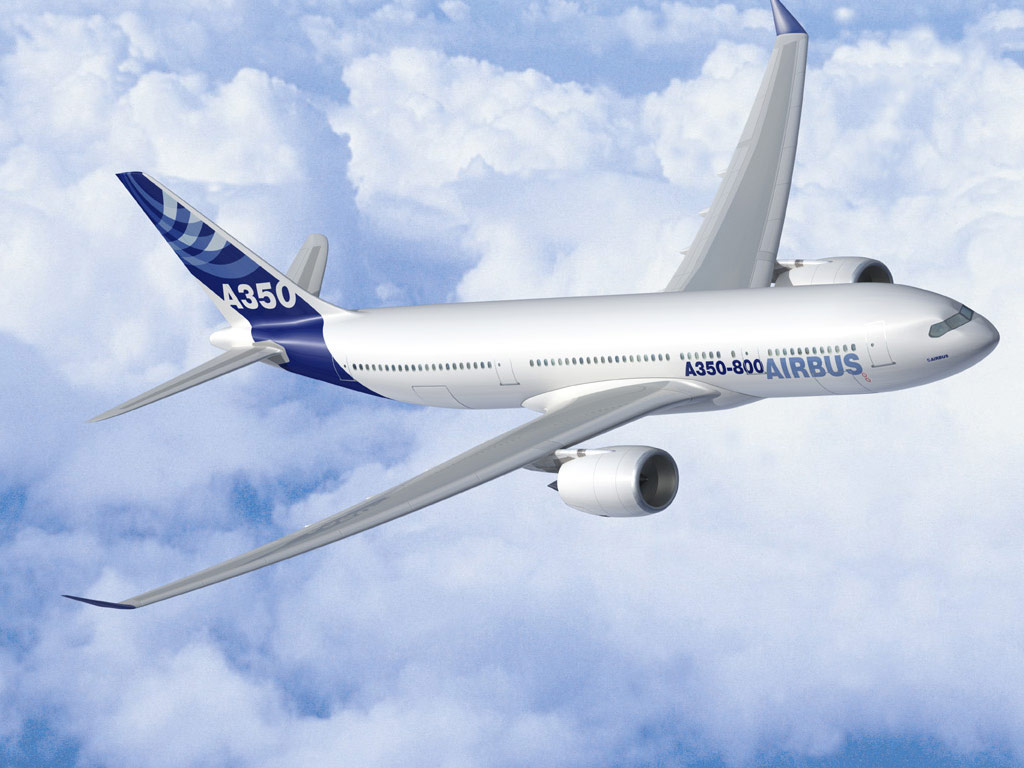
\includegraphics[height=50mm]{Figures/Airbus_A350.jpg}

% Title, author and degree
\vspace{1.0cm}
{\FontLb Thesis Title} \\ % <<<<< EDIT TITLE
%\vspace{0.2cm}
%{\FontMn Subtitle (optional)} \\
%\vspace{1.9cm}
\vspace{2.6cm}
{\FontMb Candidate Full Name} \\ % <<<<< EDIT NAME
\vspace{2.0cm}
{\FontSn \coverThesis} \\
\vspace{0.3cm}
{\FontLb Aerospace Engineering} \\ % <<<<< EDIT COURSE
\vspace{1.0cm}
{\FontSn %
\begin{tabular}{ll}
 \coverSupervisors: & Prof. Full Name 1 \\ % <<<<< EDIT NAME
                    & Dr. Full Name 2    % <<<<< EDIT NAME
\end{tabular} } \\
\vspace{1.0cm}
{\FontMb \coverExaminationCommittee} \\
\vspace{0.3cm}
{\FontSn %
\begin{tabular}{c}
\coverChairperson:     Prof. Full Name          \\ % <<<<< EDIT NAME
\coverSupervisor:      Prof. Full Name 1 (or 2) \\ % <<<<< EDIT NAME
\coverMemberCommittee: Prof. Full Name 3           % <<<<< EDIT NAME
\end{tabular} } \\
\vspace{1.5cm}
{\FontMb Month Year} \\ % <<<<< EDIT DATE (corresponds to date of oral examination)
%
\end{center}

 % file "Thesis_FrontCover.tex"
\cleardoublepage

% ----------------------------------------------------------------------
% Dedication page (optional)
% ----------------------------------------------------------------------
%%%%%%%%%%%%%%%%%%%%%%%%%%%%%%%%%%%%%%%%%%%%%%%%%%%%%%%%%%%%%%%%%%%%%%%%
%                                                                      %
%     File: Thesis_Dedication.tex                                      %
%     Tex Master: Thesis.tex                                           %
%                                                                      %
%     Author: Andre C. Marta                                           %
%     Last modified :  2 Jul 2015                                      %
%                                                                      %
%%%%%%%%%%%%%%%%%%%%%%%%%%%%%%%%%%%%%%%%%%%%%%%%%%%%%%%%%%%%%%%%%%%%%%%%

\null\vskip5cm%
\begin{flushright}
     Dedicated to someone special...
\end{flushright}
\vfill\newpage

 % file "Thesis_Dedication.tex"
\cleardoublepage

% ----------------------------------------------------------------------
%  Acknowledgments (optional)
% ----------------------------------------------------------------------
%%%%%%%%%%%%%%%%%%%%%%%%%%%%%%%%%%%%%%%%%%%%%%%%%%%%%%%%%%%%%%%%%%%%%%%%
%                                                                      %
%     File: Thesis_Acknowledgments.tex                                 %
%     Tex Master: Thesis.tex                                           %
%                                                                      %
%     Author: Andre C. Marta                                           %
%     Last modified :  2 Jul 2015                                      %
%                                                                      %
%%%%%%%%%%%%%%%%%%%%%%%%%%%%%%%%%%%%%%%%%%%%%%%%%%%%%%%%%%%%%%%%%%%%%%%%

\section*{\acknowledgments}

% Add entry in the table of contents as section
\addcontentsline{toc}{section}{\acknowledgments}

A few words about the university, financial support, research advisor, dissertation readers, faculty or other professors, lab mates, other friends and family...

 % file "Thesis_Acknowledgements.tex"
\cleardoublepage

% ----------------------------------------------------------------------
%  Abstract (both in English and Portuguese)
% ----------------------------------------------------------------------
%%%%%%%%%%%%%%%%%%%%%%%%%%%%%%%%%%%%%%%%%%%%%%%%%%%%%%%%%%%%%%%%%%%%%%%%
%                                                                      %
%     File: Thesis_Resumo.tex                                          %
%     Tex Master: Thesis.tex                                           %
%                                                                      %
%     Author: Andre C. Marta                                           %
%     Last modified :  2 Jul 2015                                      %
%                                                                      %
%%%%%%%%%%%%%%%%%%%%%%%%%%%%%%%%%%%%%%%%%%%%%%%%%%%%%%%%%%%%%%%%%%%%%%%%

\section*{Resumo}

% Add entry in the table of contents as section
\addcontentsline{toc}{section}{Resumo}

Nós apresentamos um algoritmo para a criação de uma hierarquia multinível no espaço dos raios de raios coerentes que corre no GPU. O nosso algoritmo usa rasterização para processar os raios primários e posteriormente usa esses resultados como entrada para a criação da hierarquia de raios secundários. O algoritmo gera um conjunto de raios; cria índices para esses raios, de acordo com os seus atributos; e ordena-os. Deste modo geramos uma lista de raios que são coerentes com os seus adjacentes. Para melhorar o desempenho ainda mais, subdividimos a geometria da cena num conjunto de esferas envolventes que são posteriormente intersectadas com a hierarquia de raios para diminuir o número de falsos positivos nos testes de intersecção com primitivas. Demonstramos que a nossa técnica diminui de forma notável o número de intersecções entre primitivas necessárias para renderizar uma imagem, em particular até cerca de 50\% menos do que outros algoritmos nesta classe.

\vfill

\textbf{\Large Palavras-chave:} {Rasterização, Ray-Tracing, Indexaçao de Raios, Ordenamento de Raios, Cone Envolvente, Esfera Envolvente, Hierarquias, GPU, GPGPU}   % file "Thesis_Resumo.tex"
\cleardoublepage

%%%%%%%%%%%%%%%%%%%%%%%%%%%%%%%%%%%%%%%%%%%%%%%%%%%%%%%%%%%%%%%%%%%%%%%%
%                                                                      %
%     File: Thesis_Abstract.tex                                        %
%     Tex Master: Thesis.tex                                           %
%                                                                      %
%     Author: Andre C. Marta                                           %
%     Last modified :  2 Jul 2015                                      %
%                                                                      %
%%%%%%%%%%%%%%%%%%%%%%%%%%%%%%%%%%%%%%%%%%%%%%%%%%%%%%%%%%%%%%%%%%%%%%%%

\section*{Abstract}

% Add entry in the table of contents as section
\addcontentsline{toc}{section}{Abstract}

Insert your abstract here with a maximum of 250 words, followed by 4 to 6 keywords...

\vfill

\textbf{\Large Keywords:} keyword1, keyword2,...

 % file "Thesis_Abstract.tex"
\cleardoublepage

% ----------------------------------------------------------------------
%  Table of contents, list of tables, list of figures and nomenclature
% ----------------------------------------------------------------------

% Table of contents
%
\tableofcontents
\cleardoublepage 

% List of tables
%
% Add entry in the table of contents as section
\phantomsection
\addcontentsline{toc}{section}{\listtablename}
% Generate list
\listoftables
\cleardoublepage 

% List of figures
%
% Add entry in the table of contents as section
\phantomsection
\addcontentsline{toc}{section}{\listfigurename}
% Generate list
\listoffigures
\cleardoublepage 

% Nomenclature
%
% entries of nomenclature list
%%%%%%%%%%%%%%%%%%%%%%%%%%%%%%%%%%%%%%%%%%%%%%%%%%%%%%%%%%%%%%%%%%%%%%%%
%                                                                      %
%     File: Thesis_Nomenclature.tex                                    %
%     Tex Master: Thesis.tex                                           %
%                                                                      %
%     Author: Andre C. Marta                                           %
%     Last modified : 21 Jan 2011                                      %
%                                                                      %
%%%%%%%%%%%%%%%%%%%%%%%%%%%%%%%%%%%%%%%%%%%%%%%%%%%%%%%%%%%%%%%%%%%%%%%%
%
% The definitions can be placed anywhere in the document body
% and their order is sorted by <symbol> automatically when
% calling makeindex in the makefile
%
% The \glossary command has the following syntax:
%
% \glossary{entry}
%
% The \nomenclature command has the following syntax:
%
% \nomenclature[<prefix>]{<symbol>}{<description>}
%
% where <prefix> is used for fine tuning the sort order,
% <symbol> is the symbol to be described, and <description> is
% the actual description.

% ----------------------------------------------------------------------
% Abbreviations [A]

\nomenclature[A]{GPU}{Graphics Processing Unit}
\nomenclature[A]{GPGPU}{General-purpose computing on Graphics Processing Units}

\nomenclature[A]{RSH}{Ray-Space Hierarchy}
 % file "Thesis_Nomenclature.tex"
%
% Add entry in the table of contents as section
\phantomsection
\addcontentsline{toc}{section}{\nomname}
% Insert glossary/nomenclature section produced by MakeIndex
\printnomenclature
\cleardoublepage

% Set arabic numbering (1,2,...) after preface
%
\setcounter{page}{1}
\pagenumbering{arabic}

% ----------------------------------------------------------------------
%  Chapters
% ----------------------------------------------------------------------

%%%%%%%%%%%%%%%%%%%%%%%%%%%%%%%%%%%%%%%%%%%%%%%%%%%%%%%%%%%%%%%%%%%%%%%%
%                                                                      %
%     File: Thesis_Introduction.tex                                    %
%     Tex Master: Thesis.tex                                           %
%                                                                      %
%     Author: Andre C. Marta                                           %
%     Last modified :  2 Jul 2015                                      %
%                                                                      %
%%%%%%%%%%%%%%%%%%%%%%%%%%%%%%%%%%%%%%%%%%%%%%%%%%%%%%%%%%%%%%%%%%%%%%%%

\chapter{Introduction}
\label{chapter:introduction}

Insert your chapter material here...

%%%%%%%%%%%%%%%%%%%%%%%%%%%%%%%%%%%%%%%%%%%%%%%%%%%%%%%%%%%%%%%%%%%%%%%%
\section{Motivation}
\label{section:motivation}

Relevance of the subject...


%%%%%%%%%%%%%%%%%%%%%%%%%%%%%%%%%%%%%%%%%%%%%%%%%%%%%%%%%%%%%%%%%%%%%%%%
\section{Topic Overview}
\label{section:overview}

Provide an overview of the topic to be studied...


%%%%%%%%%%%%%%%%%%%%%%%%%%%%%%%%%%%%%%%%%%%%%%%%%%%%%%%%%%%%%%%%%%%%%%%%
\section{Objectives}
\label{section:objectives}

Explicitly state the objectives set to be achieved with this thesis...


%%%%%%%%%%%%%%%%%%%%%%%%%%%%%%%%%%%%%%%%%%%%%%%%%%%%%%%%%%%%%%%%%%%%%%%%
\section{Thesis Outline}
\label{section:outline}

Briefly explain the contents of the different chapters...

 % file "Thesis_Introduction.tex"
\cleardoublepage

%%%%%%%%%%%%%%%%%%%%%%%%%%%%%%%%%%%%%%%%%%%%%%%%%%%%%%%%%%%%%%%%%%%%%%%%
%                                                                      %
%     File: Thesis_Background.tex                                      %
%     Tex Master: Thesis.tex                                           %
%                                                                      %
%     Author: Andre C. Marta                                           %
%     Last modified :  2 Jul 2015                                      %
%                                                                      %
%%%%%%%%%%%%%%%%%%%%%%%%%%%%%%%%%%%%%%%%%%%%%%%%%%%%%%%%%%%%%%%%%%%%%%%%

\chapter{Background}
\label{chapter:background}

%%%%%%%%%%%%%%%%%%%%%%%%%%%%%%%%%%%%%%%%%%%%%%%%%%%%%%%%%%%%%%%%%%%%%%%%
\section{Ray-Tracing}
\label{section:background_ray_tracing}

Ray-tracing \cite{Whitted80} is a global illumination \cite{Ritschel12} technique that is used for the synthesis of realistic images which employs recursive ray-casting \cite{Appel68}.

\medskip

The ray tracing algorithm casts primary rays from the eye but does not stop there. 
When the rays intersect geometry they can generate extra secondary rays: e.g. shadow, reflection and refraction rays.

\begin{figure}[!htb]
    \centering
    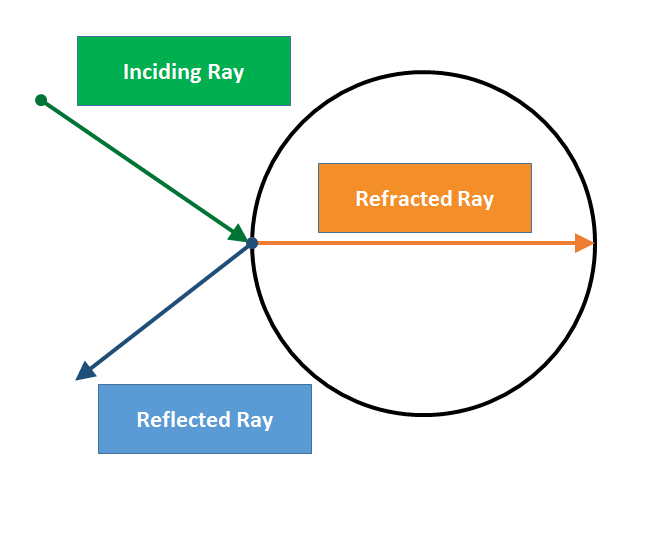
\includegraphics[scale=0.65]{Images/Secondary_Rays}
    \caption{\label{fig:bscr}Secondary Rays}
\end{figure}

These rays differentiate ray-tracing from the more traditional rasterization algorithm since they naturally allow realistic and complex effects like reflections, refractions and shadows without any need for additional techniques. However this comes with at price. Ray-tracing is computationally expensive. There is extensive research and ongoing to try and optimize it. Much of this research involves creating hierarchies in either the Object or Spatial domains to decrease the number of intersection tests in a divide and conquer fashion.

\medskip

Object and Spatial Hierarchies (like Octrees and Bounding Volume Hierarchies) help reduce the amount of intersections by reducing the amount of scene geometry required to test by culling many polygons and objects away from the ray paths at once (see Figure~\ref{fig:octree} and Figure~\ref{fig:bvh}).

\begin{figure}[!htb]
    \begin{minipage}{0.475\linewidth}
        \centering
        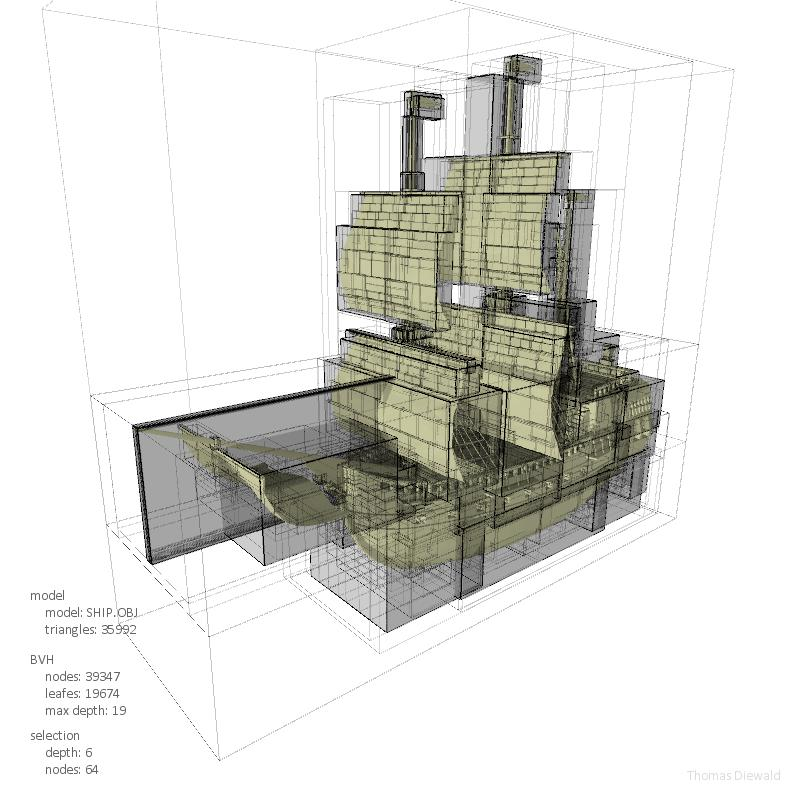
\includegraphics[width=6.0cm]{Images/BVH_Render}
        \captionof{figure}{\label{fig:octree}Octree}
    \end{minipage}
    \begin{minipage}{0.475\linewidth}
        \centering
        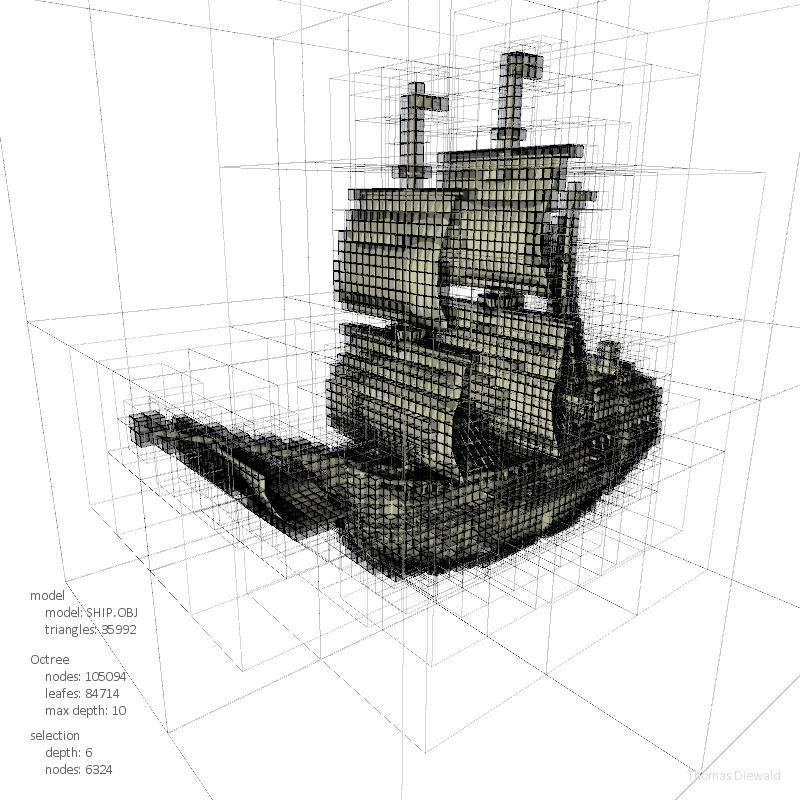
\includegraphics[width=6.0cm]{Images/Octree_Render}
        \captionof{figure}{\label{fig:bvh}Bounding Volume Hierarchy}    
    \end{minipage}
\end{figure}

Ray-Space Hierarchies, use ray bundles or ray caching mechanisms to achieve the same goal, reduce the number of intersections. Instead of creating hierarchies based on the scenes geometry, they are based on the rays being cast in each frame. This is the approach we decided to take is based on ray bundling but also uses a feature of ray caching, which is ray hashing \cite{Arvo87} \cite{Aila10}.

\begin{figure}[!htb]
    \begin{minipage}{0.475\linewidth}
        \centering
        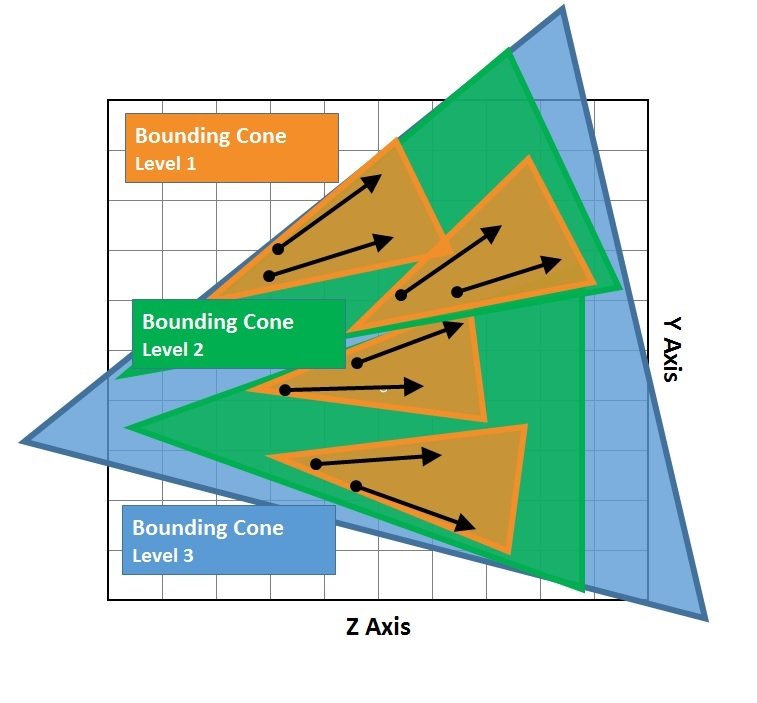
\includegraphics[width=6.0cm]{Images/Bounding_Cone}
        \captionof{figure}{\label{fig:bbc}Bounding Cone}
    \end{minipage}
    \begin{minipage}{0.475\linewidth}
        \centering
        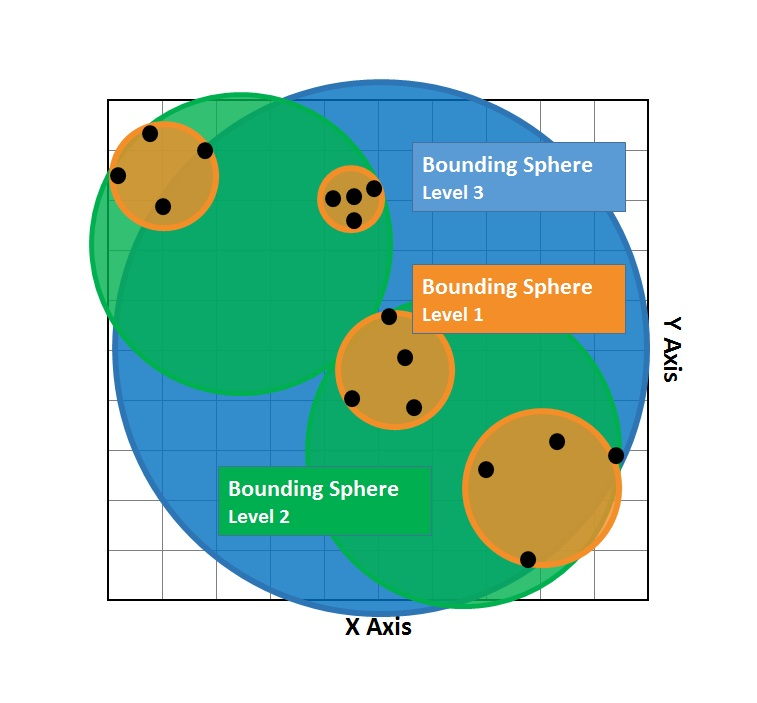
\includegraphics[width=6.0cm]{Images/Bounding_Sphere}
        \captionof{figure}{\label{fig:bbs}Bounding Sphere}    
    \end{minipage}
\end{figure}

\pagebreak

%%%%%%%%%%%%%%%%%%%%%%%%%%%%%%%%%%%%%%%%%%%%%%%%%%%%%%%%%%%%%%%%%%%%%%%%
\section{Fast Ray Tracing by Ray Classification}
\label{section:backgroud_arvo97}

Arvo and Kirk \cite{Arvo87} introduced a 5-dimensional ray-space hierarchy. They subdivided the ray-space in such a way that all relevant rays are distributed among equivalence classes. These classes are associated with a candidate object set. For example, the candidate set C\textsubscript{i} contains the objects that the rays in the equivalence class E\textsubscript{i} can intersect. The focus of this algorithm is to decrease the number of intersection tests.

\medskip

Since this algorithm works in a 5-dimensional space, the first thing we need to know is which are the degrees of freedom that a ray actually has. Traditionally rays are represented by a point and a vector in a 3-dimensional space, representing its origin and its direction. However a ray only has 5 degrees of freedom. These 5 degrees are its origin, which accounts for 3 degrees, and its direction, which accounts for 2 degrees when using spherical coordinates. This allowed Arvo and Kirk to parametrize rays and thus create subsets of the rays 5-dimensional space in such a way that rays with similar origins and directions would be in the same subset. 

\medskip

The algorithm was broken into 5 steps that I will now describe. It is also important to note that the first step is only carried out once while the second and third steps are consistently carried out in order to refine the hierarchy.

\subsubsection{1. Bounding Volume Creation}

The first step is to find the 5-dimensional bounding volume that contains the equivalent of each ray that can interact with the environment in said space. Since it's important to use volumes that don't take up too much space they chose to store 5 ordered pairs that represent intervals in the 5 orthogonal axes, which they labeled x,y,z,u and v. These 5 ordered pairs represent a bounding volume. Each of these bounding volumes, denominated hypercubes, have a representation in 3-dimensional space which they call a beam. This is vital to the algorithm because this beam comprises the points in 3-dimensional space that the set of rays contained in the hypercube can reach. One of the issues however is that the beams associated with the hypercubes are not generally polyhedra. To account for this fact, they used 6 different mappings that have the desired properties locally and together contain the whole ray-space. Each of the 6 mappings correspond to a dominant axis, x+,x-,y+,y-,z+ or z-, and one sixth of the direction space. The bounding volume is then created by creating six copies of the bounding volume created from the bounding box containing all the geometry. The rays are then mapped onto these bounding volumes.

\subsubsection{2. Space Subdivision}

The second step is to subdivide the 5-dimensional space into equivalence classes. The smaller each hypercube is, the more likely rays are to behave coherently. However, the smaller each hypercube is, the more classes we will have. The goal is to have hypercubes sufficiently small so that the rays of the corresponding beams intersect approximately the same objects, allowing the rays in that beam to share a set of candidate objects. Starting with the 6 bounding volumes created earlier, the hierarchy is created by subdividing each hypercube in half at each level, cycling each of the 5 axis. This continues until either the hypercubes size or the sets number of candidate objects fall below a fixed threshold. It is important to note that hypercubes are only subdivided if they contain rays generated during the ray-tracing process.

\subsubsection{3. Candidate set Creation}

For the third step each objects bounding box is intersected with the beam associated with the hypercube being tested. If there is an intersection then the object is added to that hypercubes candidate set. As the space is subdivided the candidate sets for the child hypercubes must be updated. Since there is an overlap between parent and child hypercubes they found that re-evaluating the candidate sets should only be done only after the hypercubes have been divided on all of the 5 axis, meaning a re-evaluation only after 5 subdivisions have occurred.

\subsubsection{4. Ray Classification}

The fourth step consists of finding the 5-dimensional hypercube that each ray corresponds to. This is done by mapping the ray to the 5-dimensional space and then traversing the ray-space hierarchy, beginning with the hypercube that is indexed by the rays dominant axis (this hypercube is one of the 6 copies created at the start of the algorithm) until the leaf containing the ray is reached. If the candidate set corresponding to this leaf is empty then the ray intersects nothing. Otherwise, we proceed to the next step.

\subsubsection{5. Intersection Tests}	

Finally the ray is tested with each object for intersections. Initially a coarse intersection test is carried out by using the objects bounding volume instead of the actual object, in order to reject rays that don't intersect the object.

\subsection{Considerations}

This algorithm works similarly to a Hash Tree, in the sense that each ray is converted to a key (in this case the corresponding 5-dimensional point) and after finding out which class it belong to (the classes can be associated with the equivalence classes) it is then mapped to a value (in this case the candidate object set). For dynamic scenes it would be necessary to recalculate the candidate sets each time the objects moved, which would be very costly. This means that the ray-space hierarchy is tightly connected to the objects and their positioning in the scene. This suggests that the algorithm is not a very good fit for ray-tracing of dynamic scenes, which is my goal. The ray caching scheme is interesting however if used differently, i.e. for the sorting of secondary rays.

\vfill

%%%%%%%%%%%%%%%%%%%%%%%%%%%%%%%%%%%%%%%%%%%%%%%%%%%%%%%%%%%%%%%%%%%%%%%%
\section{Five-dimensional Adaptive Subdivision for Ray Tracing}
\label{section:backgroud_simiakakis94}

Simiakakis and Day \cite{Simiakakis94} introduced some improvements to Arvo and Kirks work \cite{Arvo87}. These improvements consist of using a directional subdivision method, which adapts automatically according to the scene. They also introduced a memory saving scheme but the main issues with Arvo and Kirks paper with dynamic scenes still remain, which does not make this algorithm a good fit for dynamic scenes.

%%%%%%%%%%%%%%%%%%%%%%%%%%%%%%%%%%%%%%%%%%%%%%%%%%%%%%%%%%%%%%%%%%%%%%%%
\section{Whitted Ray-Tracing for Dynamic Scenes using a Ray-Space Hierarchy on the GPU}
\label{section:backgroud_roger07}

Roger et al. \cite{Roger07} presented an algorithm for interactive rendering of animated scenes with Whitted Ray-Tracing. This algorithm ran fully on the GPU and focuses on the secondary rays, using the GPU rasterizer to process the primary rays. They use a ray-space hierarchy that bundles rays together using cones and spheres. The algorithm is mapped on the GPU using textures to pass information between each of the algorithms phases.

\medskip

The algorithm consists of 5 steps that i will describe. It is important to keep in mind that the first step uses the GPU rasterizer since it has the same effect as tracing the primary rays but rasterizing them is faster.

\subsubsection{Render the Scene using the Rasterizer}

This step is done using the traditional rasterizer (for example using modern OpenGLs rasterization pipeline) that outputs the pixel color, without any kind of secondary ray effects like shadows,  reflections and refractions. Like it was stated  before, the primary rays give us the same pixel color as the standard rasterizer, so they took advantage of the performance of the rasterizer to speed-up the algorithm.

\subsubsection{Generate the first set of Secondary Rays}

Since fragment shaders can have multiple render targets, they take advantage of this fact to output the initial set of secondary rays as well. These rays can consist of the shadow rays, reflection rays and refraction rays.. Since the algorithm is generic enough, it does not matter which kind of secondary rays are used. It is also worth noting that the shadow rays are very coherent locally (if we're using soft shadows) so they fit cone hierarchy quite well.

\subsubsection{Build the Ray-Space Hierarchy}

The second step is taking the rays generated from the previous step and constructing the hierarchy. Each node consists of a structure composed by a sphere and a cone, which means that 8 floats are stored, 3 for spheres center and 1 for the spheres radius, 3 for the cones direction and 1 for the cones spread angle.i The hierarchy is constructed bottom-up, meaning that the leaves are constructed first. These leaves consist of spheres with radii 0 and cones with spread 0, representing the exact rays. The upper levels are then constructed by computing the union of the child nodes until we have a top node that encloses the whole ray-space.

\subsubsection{Intersect the Ray-Space Hierarchy with the Scene}

In this step the ray-space hierarchy is intersected with the scene. This is done in a top-down manner, testing each parent node before going down the hierarchy. Only triangles that intersect the parent node will be tested for intersections with the children nodes. This means that at each level of the hierarchy several triangles are removed from the intersection tests. It is also important to note that for this preliminary intersection phase the tests are carried out using the triangles bounding spheres since they are simply exclusion tests before the final local intersection tests. At each level of the hierarchy the intersection information is stored in textures, one for each of the 4 children nodes. If there is an intersection, the IDs for the triangle and the cone are stored in a texture, otherwise an empty element is stored. Since the texture will have blanks when there are failed intersection tests. These 4 textures also need pruned of empty elements  for the next pass.

\medskip

This has two purposes, one being memory management and the other being the mapping of the algorithm to the GPGPU. Since each pass stores its output in textures we can process each pass using the same operations meaning that there won't be threads having different execution paths which in turn is one of the features necessary to make an algorithm fit the GPU. These pruning methods are called stream-reduction passes and they presented two different methods, one involving an hierarchical version of Horns \cite{GPUGems2} and a slower one using geometry shaders. The hierarchical version works by breaking down the textures in components of fixed size and concatenating them at the end.

\subsubsection{Final Intersection Tests}	

Finally after traversing the hierarchy we have a texture with the triangle and  ray IDs (the last level of the hierarchy are individual rays), which means we need to calculate the traditional intersection tests, keeping the closest intersection.

\subsubsection{Considerations}

This algorithm works as a bounding volume hierarchy of sorts, adapted to the rays, using cones and spheres to enclose the ray bundles. It is also very well adapted to GPGPU since each pass has a fixed number of operations and has the same execution path. The stream-pass reduction method is vital since it helps prune the textures of empty elements, allowing the threads processing the textures to execute the same operations. Finally it leaves the possibility of combining the ray-space hierarchy with a object-space hierarchy, possibly reducing the number of intersections even more. It is also an example of hybrid rendering since it uses the GPUs rasterizer to compute the initial rays and the initial set of secondary rays.

\vfill

%%%%%%%%%%%%%%%%%%%%%%%%%%%%%%%%%%%%%%%%%%%%%%%%%%%%%%%%%%%%%%%%%%%%%%%%
\section{Fast Ray Sorting and Breadth-First Packet Traversal for GPU Ray Tracing}
\label{section:backgroud_garanzha10}

Garanzha and Loop \cite{Garanzha10} introduced an algorithm using various parallel primitives to adapt the ray-tracing algorithm to the GPU. Their algorithm sorts the generated rays and creates tight-fit frustums on the GPU and then intersects them with a Bounding Volume Hierarchy for the scenes geometry that is built on the CPU. One of the most interesting parts of their work is the fast ray sorting since it is done using parallel primitives which mitigates the overall cost of the operation when its executed on the GPU. I will now go into more detail regarding the four stages of the algorithm that they outlined.

\medskip

\subsubsection{Ray Sorting}

The first step, Ray Sorting, is used to store coherent rays in coherent memory locations in order to have less divergence during the tracing routine. If any given set of rays are coherent, they are more likely to intersect the same geometry and thus access the same memory locations. The sorting also allows the frustums in the next step to be tighter fits and thus give us a smaller set of intersection candidates.

\medskip

To sort the rays, they created a key-index pair for each ray, with the key being the rays ID and the index being the rays Hash value. This hash value is computed by quantizing the rays origin in a virtual grid that is within the scenes bounding box and then by quantizing its direction using a similar process.
After creating this pair for every ray, a compression-sorting-decompression scheme is used. This compression step generates chunks out of the initial set of rays. These chunks are represented by three arrays, the hash array (which indicates hash each chunk), the base array (which indicates the index of the first ray in each chunk) and a size array. This compression step takes advantage of the fact that it is likely that rays that are generated sequentially will have the same hash value. These chunks are then sorted using radix sort. The final step is the decompression, which applies an exclusive scan on the chunks size array to generate an array that indicates where each chunk will start in the re-ordered rays set.
After the exclusive scan two arrays are generated, the skeleton array that contains the base of the chunk in the positions from which the re-ordered rays set will be created from and the head flags array that indicates where new chunks start. An inclusive segment scan is then applied to these two arrays and the final re-ordered ray set is built. The final part of the decompression step is extracting the ranges of the packets of coherent rays. This is done by compressing the re-ordered ray set, using the same procedure that was used for the un-ordered ray set and then dividing those compressed chunks into packets, with a maximum size that is defined manually and then by decompressing using an inclusive segmented scan once more.

\subsubsection{Frustum Creation}

The frustum creation step picks up where the sorting left off. From the packet ranges calculated in the previous step a frustum is created for each one, using a dominant axis and two axis aligned rectangles to represent them, bounding each ray in the packet.

\subsubsection{Frustum Traversal}

The frustums are then intersected with the scenes Bounding Volume Hierarchy that was created on the CPU. This binary BVH has arity eight and 2/3rds of the tree levels are eliminated and an Octo-BVH is created. After traversing the BVH in a breadth-first order, each frustum will have a list of leaves assigned to it, which contain the primitives that will be used in the next step.

\subsubsection{Local Intersection Tests}

Finally the leaves are iterated on and for each of the primitives that they contain, localized intersection tests are calculated.

\subsubsection{Considerations}

This algorithm does not create a global Ray-Space hierarchy that contains every single ray. Instead, smaller local Frustums are created, taking advantage of the Ray-Sorting step to make them tight-fits. This reduces the number of leaves that each frustum will have assigned to it after traversing the Bounding Volume Hierarchy, which in turn reduces the number of localized intersection tests. The Ray-Sorting step is very interesting as it uses parallel primitives such as segmented scans to maximize its effectiveness on the GPU. This approach can be merged with Roger et al's \cite{Roger07} algorithm in order to create a more efficient RSH. % file "Thesis_Background.tex"
\cleardoublepage

%%%%%%%%%%%%%%%%%%%%%%%%%%%%%%%%%%%%%%%%%%%%%%%%%%%%%%%%%%%%%%%%%%%%%%%%
%                                                                      %
%     File: Thesis_Implementation.tex                                  %
%     Tex Master: Thesis.tex                                           %
%                                                                      %
%     Author: Andre C. Marta                                           %
%     Last modified :  2 Jul 2015                                      %
%                                                                      %
%%%%%%%%%%%%%%%%%%%%%%%%%%%%%%%%%%%%%%%%%%%%%%%%%%%%%%%%%%%%%%%%%%%%%%%%

\chapter{Algorithm}
\label{chapter:algorithm}

Our algorithm is performed in eight steps (see Figure~\ref{fig:crsh}). In each frame steps 1 and 2 are executed just once while steps 3 through 6 are executed once per ray batch. Batches can consist of any combination of shadow rays, reflection rays or refraction rays.

\begin{figure}[!htb]
    \centering
    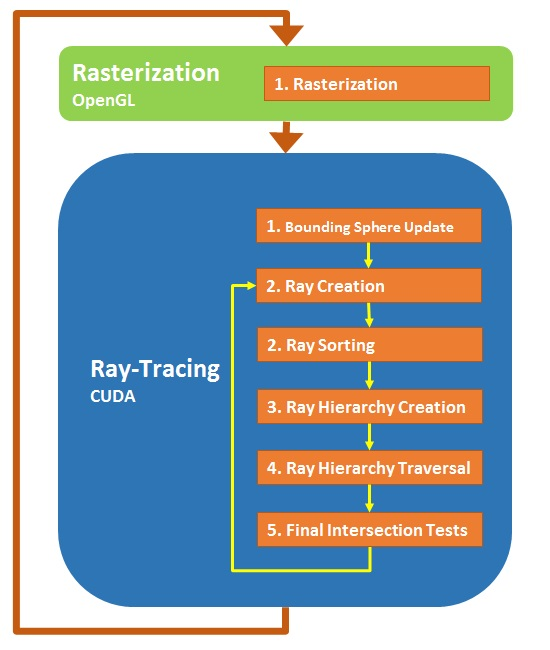
\includegraphics[width=0.45\textwidth]{Images/Overview}
    \caption{\label{fig:crsh}Coherent Ray-Space Hierarchy Overview.}
\end{figure}

%%%%%%%%%%%%%%%%%%%%%%%%%%%%%%%%%%%%%%%%%%%%%%%%%%%%%%%%%%%%%%%%%%%%%%%%
\section{Rasterization}
\label{section:algorithm-rasterization}

Rasterization is performed as a first step. There was in the path an ongoing urban legend that Rasterization and Ray-Tracing are polar opposites and that a choice has to be made between these two techniques. This is not true at all. Although Rasterization solves the rendering problem conversely vs Ray-Tracing (i.e. projecting primitives to the screen, vs projecting rays backwards to the primitives in the scene), one can complement the other. The first set of rays, the primary rays, does not convey any of the global illumination effects that Ray-Tracing is well suited to achieve, such as Shadows, Reflections and Refractions. This means that Rasterization can convey similar visual results to tracing the primary rays, while being extremely faster and optimized in the graphics hardware. Supplementing the Rasterization of primary rays with the Ray-Tracing of secondary rays can get us the benefits from both techniques: the efficiency of Rasterization and the global illumination effects from Ray-Tracing.

\medskip

In order to combine both techniques the output from the fragment shaders used to rasterize the scene must be more than just the traditional fragment colors. We need to create different render targets according to the information we want to store. In our case we output the fragment diffuse and specular properties, the fragment position and the fragment normal. In our implementation the fragment shader outputs 4 different textures containing four 32 bit floats per pixel each. These textures are generated with OpenGL/GLSL and are then sent to CUDA to create the first level of secondary rays.

%%%%%%%%%%%%%%%%%%%%%%%%%%%%%%%%%%%%%%%%%%%%%%%%%%%%%%%%%%%%%%%%%%%%%%%%
\section{Ray-Tracing}
\label{section:algorithm-ray-tracing}

\subsection{Bounding Volume Update}
Here we update the object bounding spheres according to the transformations being applied to the object they contain (e.g. translation, scale). Since we only update the center and the radius there is no need to recalculate the bounding spheres in each frame (transformations do not invalidate the bounding spheres).

We pre-compute the minimum bounding sphere of the object meshes, using an implementation based on \cite{Gartner99}s algorithm, so there is no impact on render time performance for this computation.

\subsection{Secondary Ray Generation and Indexing}

After the Rasterization step we need to generate the secondary rays. We create an index for each individual ray in order to speed up ray sorting in the following steps. We use a different hashing function for each type of ray (see Figures~\ref{fig:sr}, ~\ref{fig:rr}). Since each ray consists of an origin and a direction it would be straightforward to use these two parameters to create our hash. However for shadow rays it is sufficient to use the light-index, to which it belongs, and the ray direction. This is doable if we invert the origin of the shadow ray so that it is located at the light source rather than the originating fragment. To further reduce the size of the hash keys we convert the ray direction into spherical coordinates \cite{GraphicGems5} and store both the light index and the spherical coordinates into a 32 bit integer, with the light index having the higher bit-value such that the shadow rays are sorted according to the light source a priori.

\begin{figure}[!htb]
    \centering
    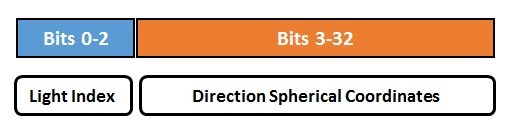
\includegraphics[scale=0.75]{Images/Shadow_Hash}
    \caption{\label{fig:sr}Shadow Ray Hash.}
\end{figure}

The Reflection and Refraction rays are also converted to spherical coordinates. However in this case the ray origin is used in the hash, given that these rays are not coherent with regards to the origin, unlike shadow rays.

\begin{figure}[!htb]
    \centering
    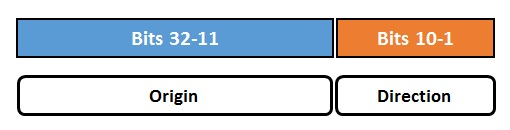
\includegraphics[scale=0.75]{Images/Reflection_Hash}
    \caption{\label{fig:rr}Reflection and Refraction Ray Hash.}
\end{figure}

Once generation is complete, we have an array with the generated secondary rays as well as two arrays with the ray keys (ray hashes) and the ray values (ray position in the ray array) and a final array with head flags which indicate if there is a ray in the corresponding position within the key-value arrays, where we store either a 0 or a 1, indicating if there is a ray or not, respectively.
Using the information from the head flags array we then run a trimming operator on the key-value arrays (see Figure~\ref{fig:at}). This is done by first applying an inclusive scan operator \cite{Merrill09} on the head flags array, which gives us the number of positions each pair needs to be shifted to the left. This is done in order to trim the arrays \cite{GPUGems2}.

\begin{figure}[!htb]
    \centering
    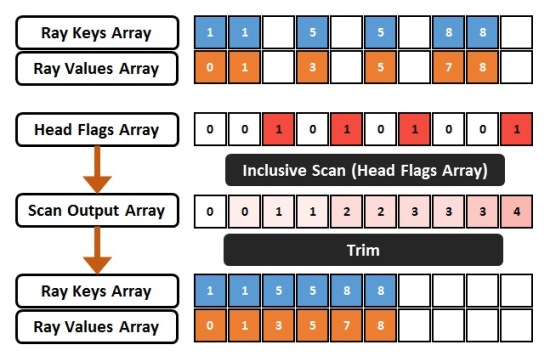
\includegraphics[scale=0.75]{Images/Array_Trimming}
    \caption{\label{fig:at}Array Trimming}
\end{figure}

\subsection{Secondary Ray Compression}

Here we use a compression-sorting-decompression scheme, expanding on prior work by Garanzha and Loops \cite{Garanzha10}. The compression step exploits the local coherency of rays. Even for secondary rays, the bounces generated by two adjacent rays have a good chance of being coherent. This can result in the same hash value for both bounces. Given this information, we compress the ray key-value pairs into chunks, minimizing the number of pairs that need to be sorted. To compress the pairs we utilize a head flags array with the same size as the key-value pair array, initializing it with $0$s in every position and inserting $1$s into positions in which the key (hash) of the corresponding pair differs from the previous pair. After populating the head flags array we apply an inclusive scan operator on it \cite{Merrill09}. By combining the head flags array with the scan output array we create the chunk keys, base and size arrays, which contain the hash, starting index and size of the corresponding chunks (see Figure~\ref{fig:rcc}). The chunk keys are represented in different colors at the image below. The chunk base array represents the original position of the first ray in the chunk while the chunk size array represents the size of the chunk, needed for the ray array decompression.

\begin{figure}[!htb]
    \centering
    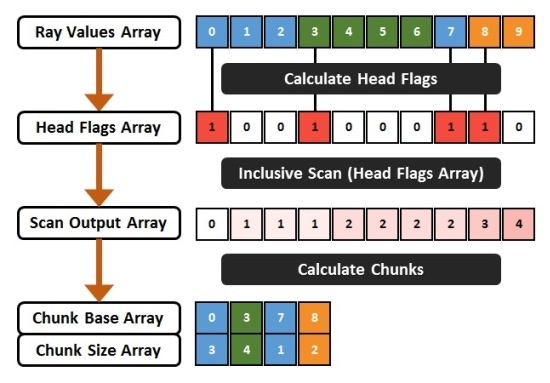
\includegraphics[scale=0.75]{Images/Ray_Compression}
    \caption{\label{fig:rcc}Ray Compression into Chunks}
\end{figure}

\subsection{Secondary Ray Sorting}

After ray compression we have an array of chunks with the information required to reconstruct the initial rays array. So we can begin the actual sorting. We radix sort \cite{Merrill11} the chunks array according to the chunk keys.

\subsection{Secondary Ray Decompression}

Decompression works by creating a skeleton array. This skeleton array is similar to the head flag arrays we created before except that it contains the size of the sorted chunks. Next we apply an exclusive scan operator on the skeleton array. This will give us the positions of the chunks starting positions on the sorted key and value arrays. After creating these two arrays for each position in the scan array we fill the sorted ray array. We start in the position indicated in the scan array and finish after filling the number of rays contained within the corresponding chunk.

\begin{figure}[!htb]
    \centering
    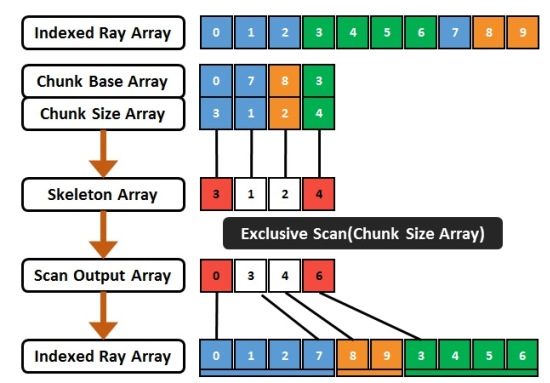
\includegraphics[scale=0.75]{Images/Ray_Decompression}
    \caption{Ray Decompression from Chunks}
\end{figure}

\subsection{Hierarchy Creation}

With the sorted rays we can now create the actual hierarchy. Since the rays are now sorted coherently the hierarchy will be much tighter in its lower levels, giving us a smaller number of intersection candidates as we traverse further down the hierarchy.
Each node in the hierarchy is represented by a sphere and a cone (see Figures~\ref{fig:bc}, \ref{fig:bs}).

\begin{figure}[!htb]
    \centering
    
    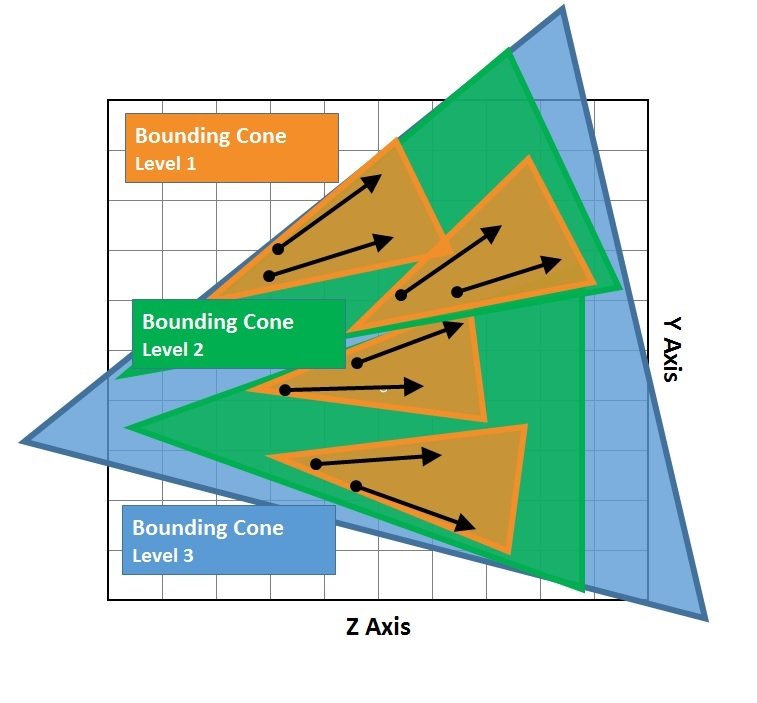
\includegraphics[scale=0.30]{Images/Bounding_Cone}
    \caption{\label{fig:bc}Bounding Cone - 2D View}

    \vspace{2.5pt}

    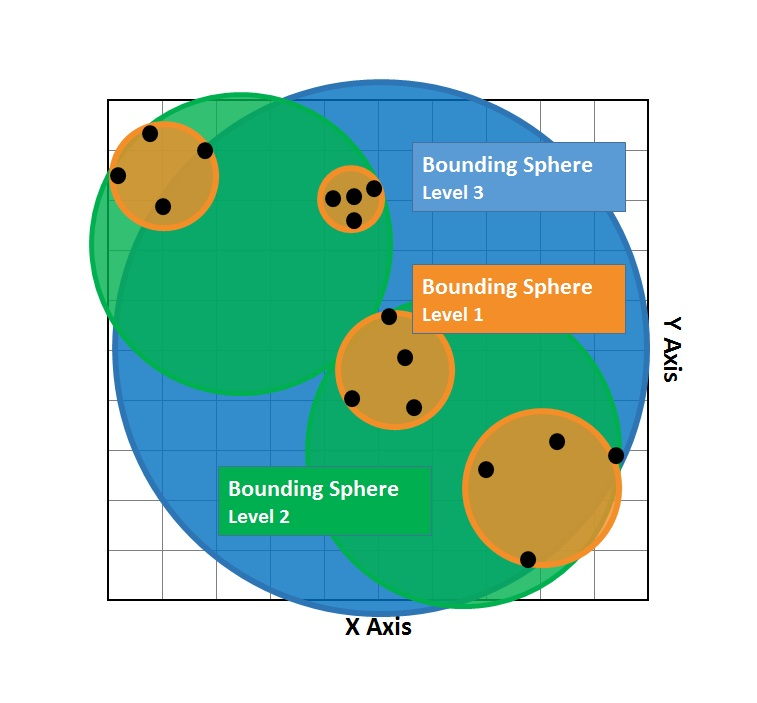
\includegraphics[scale=0.30]{Images/Bounding_Sphere}
    \caption{\label{fig:bs}Bounding Sphere - 2D View}
\end{figure}

The sphere contains all the nodes ray origins while the cone contain the rays themselves (see Figure~\ref{fig:cru}). This structure is stored using eight floats: the sphere center and radius (four floats) and the cone direction and spread angle (four floats). The construction of the hierarchy is done in a bottom-up fashion. Thus we start with the leaves, with spheres of radius $0$ and a cone with spread angle equal to $0$. These leaves correspond to the sorted rays. The upper levels of the hierarchy are created by calculating the union of the child nodes. The number of children combined in each node can also be parametrized. 

\begin{figure}[!htb]
    \centering
    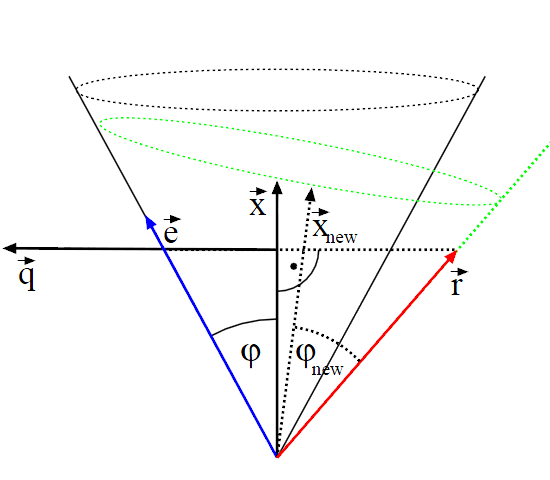
\includegraphics[scale=0.30]{Images/Cone_Union}
    \caption{\label{fig:cru}Cone-Ray Union - 2D View. \small{courtesy of \cite{Szecsi06}}.}
\end{figure}

For the first level of nodes we use the formulas below to create compact cones \cite{Szecsi06}.

\begin{equation}
    \vec{q} = \frac{ (\vec{x} \cdot \vec{r}) \cdot \vec{x} - \vec{r} }
                   {|(\vec{x} \cdot \vec{r}) \cdot \vec{x} - \vec{r}|}
\end{equation}

\begin{equation}
    \vec{e} = \vec{x} \cdot \cos(\phi) + \vec{q} \cdot \sin{\phi}
\end{equation}

\begin{equation}
    \vec{x}_{new} = \frac{ \vec{e} + \vec{r} }
                         {|\vec{e} + \vec{r}|}
\end{equation}

\begin{equation}
    \cos{\phi_{new}} = \vec{x}_{new} \cdot \vec{r}
\end{equation}

For the remaining levels we use the following formulas to combining cones:

\begin{equation}
    \vec{x}_{new} = \frac{ \vec{x_{1}} + \vec{x_{2}} }
                         {|\vec{x_{1}} + \vec{x_{2}}|}
\end{equation}

\begin{equation}        
    \cos{\phi_{new}} = \frac{\arccos(\vec{x_{1}} + \vec{x_{2}})}{2} + \max(\phi_{1}, \phi_{2})
\end{equation}

Finally for the union of spheres we use this formula:

\begin{equation}
center_{new} = \frac{center_{1} + center_{2}}{2}\\
\end{equation}
\begin{equation}
radius_{new} = \frac{|center_{2} - center_{1}|}{2} + \max(radius_{1},radius_{2})\\
\end{equation}
    
Each ray needs to know the pixel that it corresponds to. After the sorting step rays are not in their original order. We need a way to map rays back to the screen pixels. Since the hierarchy is not tied directly to the geometry positions in the scene it does not matter for hierarchy creation whether the scene is dynamic or static. The only thing which does matter is the number of bounces of each ray, meaning that if there are more pixels occupied in the screen, the hierarchy will have more nodes.

\medskip

Roger et al. \cite{Roger07} also noted that some nodes might become too large as we travel higher up into the hierarchy. To mitigate this problem we decided to limit the number of levels generated and subsequently the number of levels traversed. Since rays are sorted before this step, there is much higher coherency between rays in the lower levels. If we focus on these rays and ignore the higher levels of the hierarchy we will have better results (this will be demonstrated later in the evaluation section). There is a possibility that we might end up having more local intersection tests but since the nodes in the higher levels of the hierarchy are quite large, we would most likely end up having intersections with every single triangle. Thus having no real gain from calculating intersections on these higher level nodes to begin with.

\subsection{Hierarchy Traversal}

Once we have an hierarchy we can traverse it. Prior to traversing the hierarchy we compute the bounding spheres for each object in the scene using Bernd Gartners algorithm \cite{Gartner99}.

For the top level of the hierarchy we intersect the hierarchy nodes with the bounding spheres to cull intersections further. Finally we traverse the hierarchy in a top-down order, intersecting each node with the scenes geometry. Since the top level nodes of the hierarchy fully contain the bottom level nodes, triangles rejected at the top levels will not be tested again in the bottom level nodes. Let us say we start traversing the hierarchy with the root node. If a certain triangle does not intersect the root node then this means that that specific triangle will not intersect any of its children. Since it is the root node, it also means that no ray in the scene will intersect it so we do not have to further test it for intersections. After traversing each level of the hierarchy we store the intersection information in an array so that the child nodes will know the sets of triangles they have to compute intersections against. The intersection tests being run at this stage are only coarse grained tests. They use the triangles bounding spheres since we will have to do the actual intersection tests in the final stage anyway. The intersection tests are being run in a parallel manner so there is an issue regarding empty spaces in the textures that contain the intersection information. These arrays need to be trimmed using the same procedure that we used after the ray generation. These hits are stored as an int32 in which the first 18 bits store the node id and the last 14 bits store the triangle id. This is not a problem for larger scenes since those processed in triangle batches. Each hit only needs to store the maximum number of triangles per batch.

\begin{figure}[!htb]
    \centering
    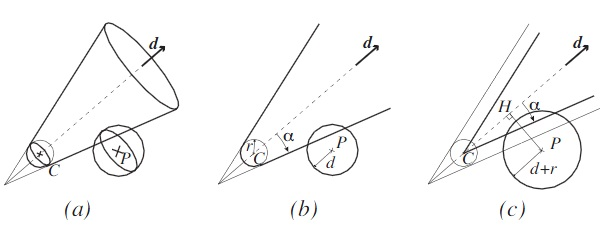
\includegraphics[scale=0.50]{Images/Node_Sphere_Intersection}
    \caption{\label{fig:crud2}Cone-Ray Union - 2D View. \small courtesy of \cite{Roger07}.}
\end{figure}

To calculate the intersection between the node, which is composed of the union of a sphere and a cone, we simplify the problem by enlarging the triangles bounding sphere \cite{Ericson04} and reducing the cones size (see Figure~\ref{fig:crud2}). The original formula for cone-sphere intersections was described in the Amanatides paper \cite{Amanatides84}. The current formula, which expands on the work of Amanatides, was described by Roger et al. \cite{Roger07}.

\begin{equation}
result = {|C - H|} \times \tan{\alpha} + \frac{d+r}{\cos{\alpha}} \geqslant
         {|P - H|}
\end{equation}

\subsection{Final Intersection Tests}

After traversing the hierarchy we have an array of node id and triangle id pairs. The candidates for the local intersection tests \cite{Moller97}. In this final step all that remains is to find out which is the closest intersected triangle for each ray and accumulate shading. Depending on the depth that we want for the algorithm we might need to output another set of secondary rays. Since the algorithm is generic, all that is necessary for this is to output these rays onto the ray array that we used initially and continue from the ray-sorting step.
 % file "Thesis_Algorithm.tex"
\cleardoublepage

%%%%%%%%%%%%%%%%%%%%%%%%%%%%%%%%%%%%%%%%%%%%%%%%%%%%%%%%%%%%%%%%%%%%%%%%
%                                                                      %
%     File: Thesis_Evaluation.tex                                      %
%     Tex Master: Thesis.tex                                           %
%                                                                      %
%     Author: Andre C. Marta                                           %
%     Last modified :  2 Jul 2015                                      %
%                                                                      %
%%%%%%%%%%%%%%%%%%%%%%%%%%%%%%%%%%%%%%%%%%%%%%%%%%%%%%%%%%%%%%%%%%%%%%%%

\chapter{Evaluation}
\label{chapter:evaluation}

%%%%%%%%%%%%%%%%%%%%%%%%%%%%%%%%%%%%%%%%%%%%%%%%%%%%%%%%%%%%%%%%%%%%%%%%
\section{Test Methodology}
\label{section:test-methodology}

We implemented our CRSH algorithm in OpenGL/C++ and CUDA/C++ then compared it with our implementation of RAH \cite{Roger07} over the same architecture. We map our algorithm onto the GPU, parallelizing it there fully. We achieve this mainly by the use of parallel primitives, like prefix sums \cite{Blelloch90}. We used the CUB \cite{Merrill09}  \cite{Merrill11} library to perform parallel radix sorts and prefix sums.

\medskip

We measure the amount of intersections, including misses and hits, to evaluate ray hierarchy algorithms proficiency at reducing the amount of ray-primitive intersection tests required to render an image. All scenes were rendered at $512\times512$ resolution. We also vary the depth of the hierarchy and the number of nodes we combine to create the upper levels of the hierarchy. We also measured the rendering time of each scene using a baseline configuration as well as the individual steps in each algorithm relatively to the overall rendering time.

\medskip

The test information was collected using a NVIDIA GeForce GTX 770M GPU with 3 GB of RAM. Our algorithm is completely executed on the GPU (including hierarchy construction and traversal) so the CPU has no impact on the test results.

%%%%%%%%%%%%%%%%%%%%%%%%%%%%%%%%%%%%%%%%%%%%%%%%%%%%%%%%%%%%%%%%%%%%%%%%
\section{Test Scenes}
\label{section:test-scenes}

We used three different scenes, \textsc{Office}, \textsc{Cornell} and \textsc{Sponza}.

\medskip

The \textsc{Office} scene (36K triangles) is representative of interior design applications. It is divided into several submeshes therefore it adapts very well to our bounding volume scheme. For this scene the emphasis was on testing shadow rays. 

\medskip

We selected \textsc{Cornell} (790 triangles). as it is representative of highly reflective scenes. It consists an object surrounded by six mirrors. On this scene we focused on testing reflection rays although it also features shadow rays in it.

\medskip

\textsc{Sponza} (66K triangles), much like \textsc{Office}, is representative of architectural scenes. For this scene the emphasis was also on testing shadow rays but for scenes that do not conform with our bounding volume scheme. This scene does not adapt well to our scheme as is not divided into submeshes. 

%%%%%%%%%%%%%%%%%%%%%%%%%%%%%%%%%%%%%%%%%%%%%%%%%%%%%%%%%%%%%%%%%%%%%%%%
\section{Test Hypothesis}
\label{section:test-hypothesis}

We hypothesised that our more coherent RSH hierarchy needs to compute fewer intersection results to render a scene. We expect more expressive results for shadow rays. As shadow rays have low divergence the sorting step should create a more coherent RSH than for reflection rays. In addition our hierarchy should also be more coherent with reflection rays than one based on the RAH algorithm due to the hashing we use. However by the very nature of reflection rays they will never be as coherent as shadow rays resulting in a lower quality hierarchy.

By varying the depth of the hierarchy we also expect that with hierarchies of a certain depth the upper nodes in the hierarchy will have degenerated so much that processing them leads to no benefit at all. In other words, these nodes will be so wide that they will intersect all the geometry in the scene, which means that we just wasted time processing them since we didn't prevent any future intersection tests. This should happen because as we go up in the hierarchy the nodes will encompass so many rays that they will be too large.

By varying the number of nodes used to create the upper levels of the hierarchy we expect a similar outcome to varying the depth. If we use more lower level nodes to create the upper level ones, the upper level nodes will be larger therefore after a certain level they will be too wide (i.e using 16 level 0 nodes to create a level 1 node). However there is a trade-off related to the memory consumption of the algorithm. If we use more nodes to create the upper nodes we will have less nodes overall and thus need less memory to store the potential intersection hits.

\vskip 27em

\pagebreak

\def\arraystretch{1.5}%  1 is the default, change whatever you need

%%%%%%%%%%%%%%%%%%%%%%%%%%%%%%%%%%%%%%%%%%%%%%%%%%%%%%%%%%%%%%%%%%%%%%%%%%%%%%%%%%%%%%%%%%%%%%%%%%%%%%%%%%%%%%%%%%%%%%%%%%%%%%%%%%
\section{Test Results and Discussion}
\label{section:test-results-and-discussion}

\subsection{Hierarchy Traversal Results - Subdivision 8 Depth 2}

\subsubsection{Office}

% Office Discussion

Comparing our algorithm with the RAH algorithm we can see that our algorithm computes 63,79\% less intersections than RAH on this scene. 98,14\% less than a brute force approach (see Table~\ref{table:office-d8-n2-results} and Table~\ref{table:results-d8-n2}).

% Office Table and Figure
    
\begin{figure}[!htb]
    \begin{minipage}{0.25\linewidth}
        \centering
        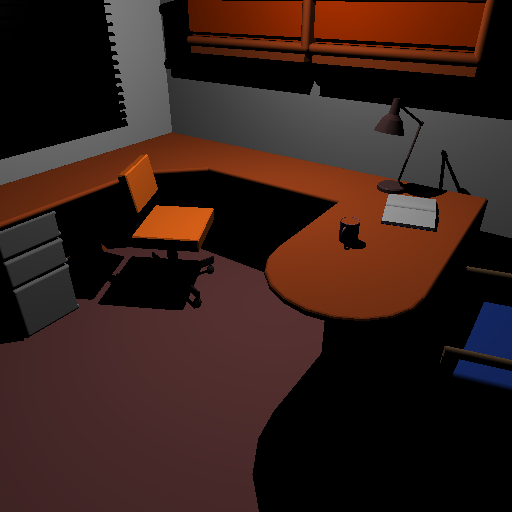
\includegraphics[width=4.0cm]{Images/Office_Preview}
        \captionof{figure}{\textsc{Office}}
    \end{minipage}
    \begin{minipage}{0.725\linewidth}
        \centering
        \fontencoding{T1}
        \fontseries{m}
        \fontshape{sc}
        \fontsize{8}{10}
        \selectfont
        \begin{tabular}[h]{l|rr}
            \multicolumn{1}{c|}{\textsc{Office}} & \textsc{Level 2} & \textsc{Level 1}\\
            \hline
            \emph{RAH Algorithm} & & \\
            \hline
            \quad \# Sh Intersections  & 142726748  & 202025920 \\
            \quad \# Sh Misses            & 117473508  & 186409563 \\
            \quad \# Sh Hits              & 25253240   & 15616357  \\
            \hline
            \emph{Our Algorithm} & & \\
            \hline
            \quad \# Sh Intersections  & 11559388   & 85572416	\\
            \quad \# Sh Misses         & 862836     & 76455023  \\
            \quad \# Sh Hits           & 10696552   & 9117393   \\
        \end{tabular}
        \label{table:office-d8-n2-results}
        \captionof{table}{\textsc{Office} Division 8 Depth 2 Test Results.}
    \end{minipage}
\end{figure}

\subsubsection{Cornell}

% Cornel Discussion

Comparing our algorithm with the RAH algorithm we can see that our algorithm computes 26,47\% less intersections than RAH on this scene. 91,17\% less than a brute force approach (see Table~\ref{table:cornell-d8-n2-results} and Table~\ref{table:results-d8-n2}).

% Cornell Table and Figure

\begin{figure}[!htb]
    \begin{minipage}{0.25\linewidth}
        \centering
        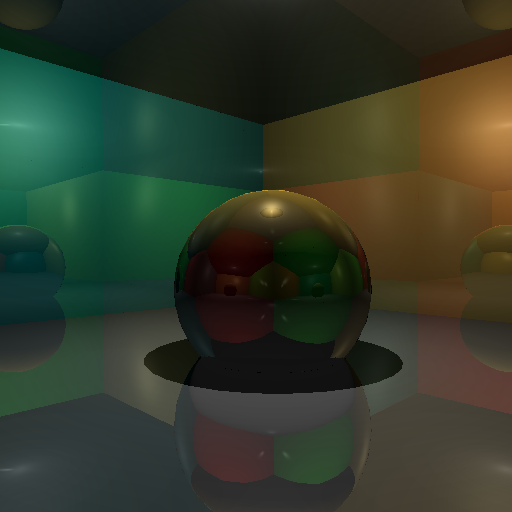
\includegraphics[width=4.0cm]{Images/Cornell_Preview}
        \captionof{figure}{\textsc{Cornell}}
    \end{minipage}
    \begin{minipage}{0.725\linewidth}
        \centering
        \fontencoding{T1}
        \fontseries{m}
        \fontshape{sc}
        \fontsize{8}{10}
        \selectfont
        \begin{tabular}[h]{l|rr}
            \multicolumn{1}{c|}{\textsc{Office}} & \textsc{Level 2} & \textsc{Level 1}\\
            \hline
            \emph{RAH Algorithm} & & \\
            \hline
            \quad \# Sh Intersections   & 2995344   & 5167632		  \\
            \quad \# Sh Misses             & 2349390   & 3606077		  \\
            \quad \# Sh Hits               & 645954    & 1561555		  \\
            & & \\
            \quad \# Re Intersections   & 6488064   & 17802296		  \\
            \quad \# Re Misses             & 4262777   & 14311812		  \\
            \quad \# Re Hits               & 2225287   & 3490484		  \\
            \hline
            \emph{Our Algorithm} & & \\
            \hline
            \quad \# Sh Intersections   & 750384    & 2375896		  \\
            \quad \# Sh Misses          & 453397    & 981144		  \\
            \quad \# Sh Hits            & 296987	& 1394752  	      \\
            & & \\
            \quad \# Re Intersections   & 2737872   & 10269256		  \\
            \quad \# Re Misses             & 1454215   & 6983410		  \\
            \quad \# Re Hits               & 1283657   & 3285846   	  \\            
        \end{tabular}
        \label{table:cornell-d8-n2-results}
        \captionof{table}{\textsc{Cornell} Division 8 Depth 2 Test Results.}
    \end{minipage}
\end{figure}

\subsubsection{Sponza}

% Sponza Discussion

Comparing our algorithm with the RAH algorithm we can see that our algorithm computes 35,86\% less intersections than RAH on this scene. 97,62\% less than a brute force approach (see Table~\ref{table:sponza-d8-n2-results} and Table~\ref{table:results-d8-n2}).

% Sponza Table and Figure

\begin{figure}[!htb]
    \begin{minipage}{0.25\linewidth}
        \centering
        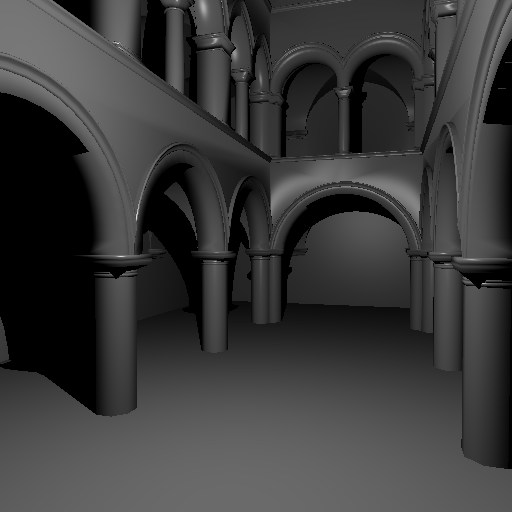
\includegraphics[width=4.0cm]{Images/Sponza_Preview}
        \captionof{figure}{\textsc{Sponza}}
    \end{minipage}
    \begin{minipage}{0.725\linewidth}
        \centering
        \fontencoding{T1}
        \fontseries{m}
        \fontshape{sc}
        \fontsize{8}{10}
        \selectfont
        \begin{tabular}[h]{l|rr}
            \multicolumn{1}{c|}{\textsc{Office}} & \textsc{Level 2} & \textsc{Level 1}\\
            \hline
            \emph{RAH Algorithm} & & \\
            \hline
            \quad \# Sh Intersections  & 266597400	& 261494752	  \\
            \quad \# Sh Misses            & 233910556  & 248455163	  \\
            \quad \# Sh Hits              & 32686844	& 13039589	  \\
            & & \\
            \hline
            \emph{Our Algorithm} & & \\
            \hline
            \quad \# Sh Intersections   & 266597400 & 62665496	  \\
            \quad \# Sh Misses          & 258764213 & 53120871	  \\
            \quad \# Sh Hits            & 7833187	& 9544625	  \\
        \end{tabular}
        \label{table:sponza-d8-n2-results}
        \captionof{table}{\textsc{Sponza} Division 8 Depth 2 Test Results.}
    \end{minipage}
\end{figure}

\subsection{Hierarchy Traversal Discussion - Subdivision 8 Depth 2}

% Comparison Table

\begin{table}[!htb]
    \begin{center}
    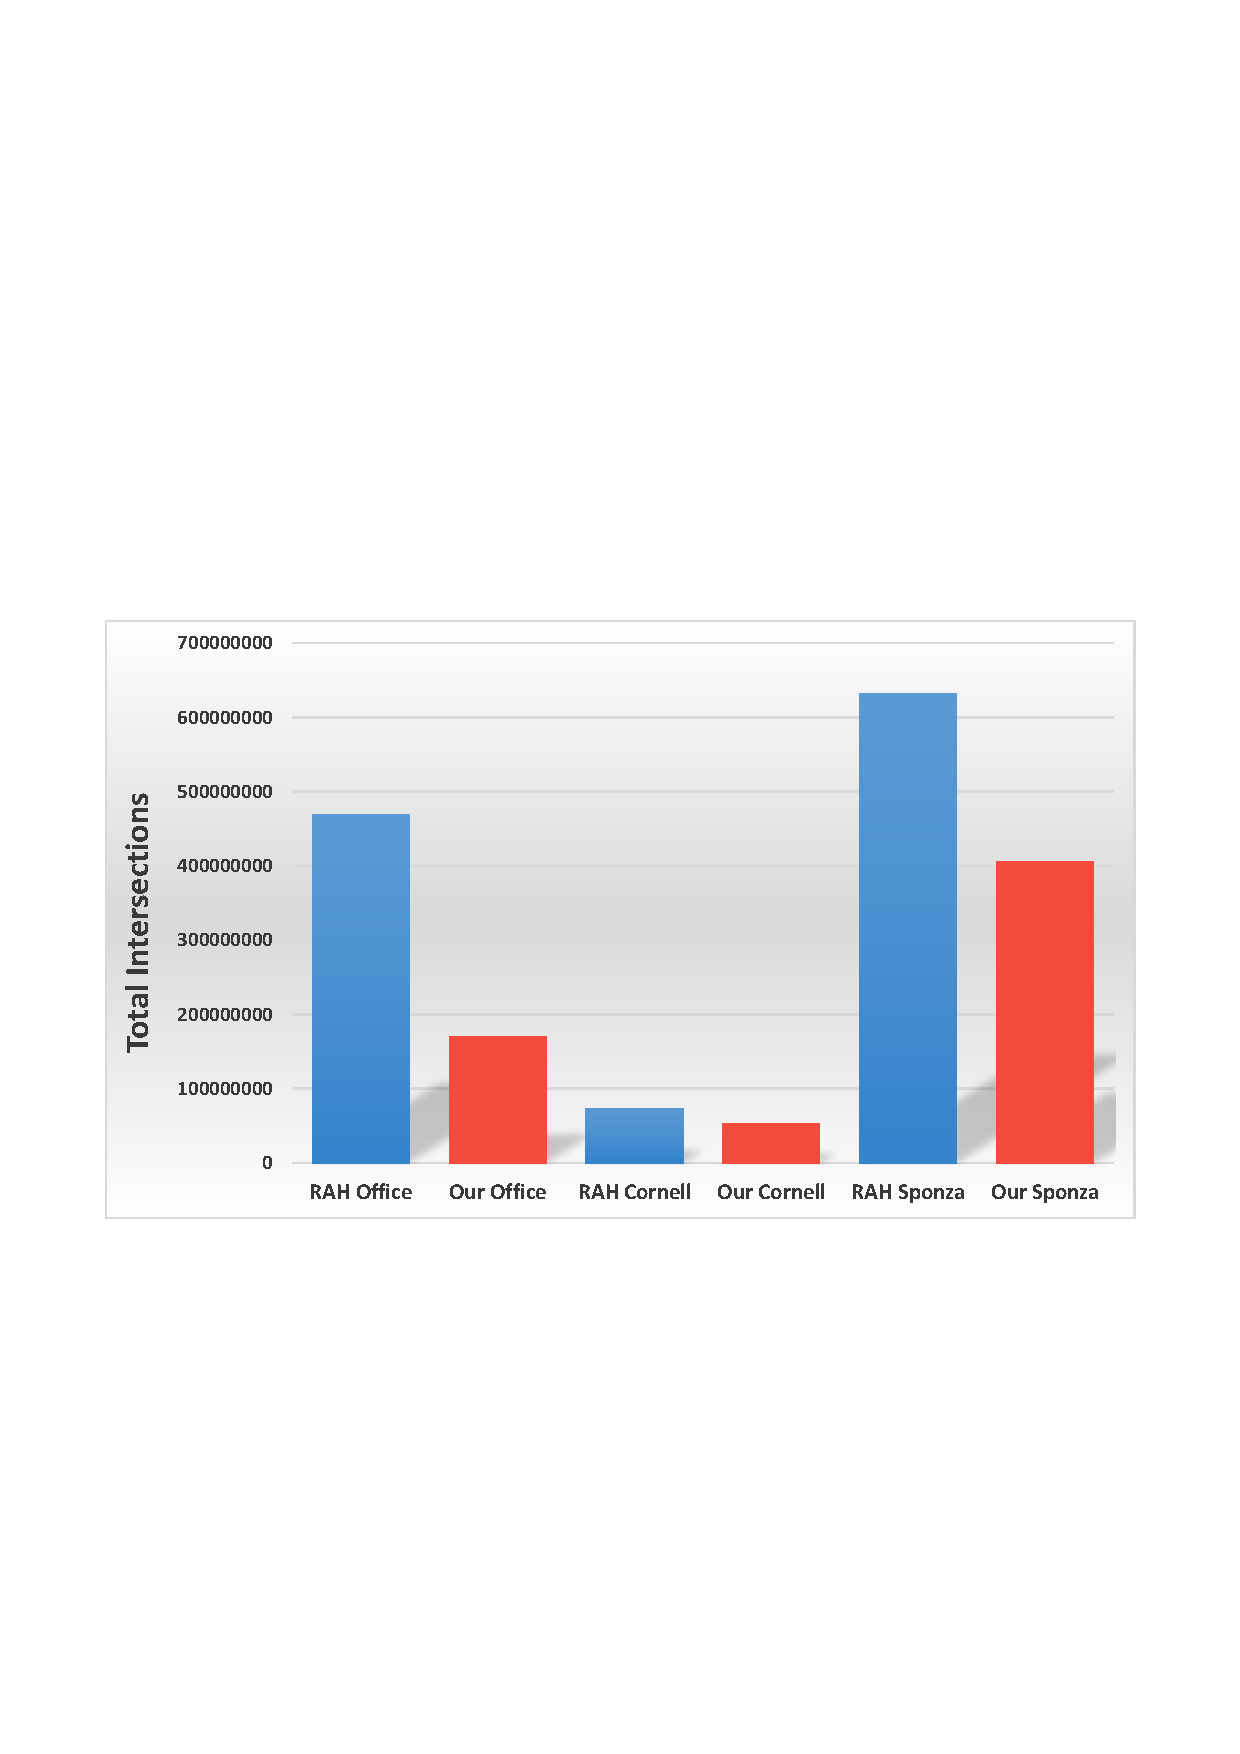
\includegraphics[width=0.85\textwidth]{Images/Chart_N8_D2}
    \vskip 2em
    \fontencoding{T1}
    \fontseries{m}
    \fontshape{sc}
    \fontsize{8}{10}
    \selectfont
    \begin{tabular}{l|rrrrrr}
    & \multicolumn{2}{c}{\textsc{Office}} & \multicolumn{2}{c}{\textsc{Cornell}} & \multicolumn{2}{c}{\textsc{Sponza}} \\
    \textsc{Algorithm} & \textsc{Total \# isect} & \textsc{Relative \%} & \textsc{Total \# isect} & \textsc{Relative \%} & \textsc{Total \# isect} & \textsc{Relative \%} \\
        \hline
        \emph{Brute Force}     & 9133132168         & 100\%           & 606911976         & 100\%           & 17058578850        & 100\% \\
        \emph{RAH Algorithm}   & 469683524		    & 5.14\%          & 72869648		  & 12.01\%         & 632408864			 & 3.71\% \\
        \emph{Our Algorithm}   & \textbf{170070948} & \textbf{1.86\%} & \textbf{53578192} & \textbf{8.83\%} & \textbf{405619896} & \textbf{2.38\%} \\
    \end{tabular}
    \end{center}
    \caption{\label{table:results-d8-n2}
    \small\textsc{Office} (251546 shadow rays), \textsc{Cornell} (242015 shadow \& 524288 reflection rays), \textsc{Sponza} (256713 shadow rays)  rendering performance using node subdivision 8 and hierarchy depth 2.}
\end{table}

For this set of tests we used a node subdivision of 8 and a hierarchy depth of 2. This means that every node in the upper levels of the hierarchy consists of 8 nodes in the level directly below (or 8 rays if we're constructing the first level of the hierarchy).

\subsubsection{Office}

Our initial expectations for Office were to get a much lower number of intersection tests with our algorithm than with RAH. The scene is a good fit to our bounding volume scheme and our highly coherent shadow ray hierarchy. Results confirm (see Table~\ref{table:office-d8-n2-results}) our initial expectations: we compute 63,79\% less intersections than RAH on this scene. 98,14\% less than a brute force approach.

\subsubsection{Cornell}

For the Cornell scene we focused primarily on the reflection rays which are much more incoherent than shadow rays so we expected results to be less positive than with the Office scene. We compute 26,47\% less intersections overall (shadow and reflection rays combined) than the RAH algorithm and 91,17\% less than the brute force approach (see Table~\ref{table:cornell-d8-n2-results}).

\subsubsection{Sponza}

The final scene, Sponza, is a whole mesh. We did not employ object subdivision in this scene. Hence we expected worse results than with Office since we would only get the benefit of the shadow ray hierarchy and none from the bounding volume scheme. We compute 35,86\% less intersection tests than RAH and 97,62\% than the brute force approach (see Table~\ref{table:sponza-d8-n2-results}). This confirmed our expectations since the results are about 50\% worse than they were with the Office. 

However even without the object subdivision our algorithm still manages to outperform RAH, which is very positive since these results all stem from the sorting we applied on the rays before creating the hierarchy.

\subsubsection{Configuration Comparison}

Since we have not analyzed the results for different subdivision and depth configurations we will only compare this setup (as a baseline) with the remaining ones in the next sections.

\vskip 15em

%%%%%%%%%%%%%%%%%%%%%%%%%%%%%%%%%%%%%%%%%%%%%%%%%%%%%%%%%%%%%%%%%%%%%%%%%%%%%%%%%%%%%%%%%%%%%%%%%%%%%%%%%%%%%%%%%%%%%%%%%%%%%%%%%%

\pagebreak
\subsection{Hierarchy Traversal Results - Subdivision 8 Depth 3}

\subsubsection{Office}

% Office Discussion

Comparing our algorithm with the RAH algorithm we can see that our algorithm computes 39,18\% less intersections than RAH on this scene. 97,87\% less than a brute force approach (see Table~\ref{table:office-d8-n3-results} and Table~\ref{table:results-d8-n3}).

% Office Table and Figure
    
\begin{figure}[!htb]
    \begin{minipage}{0.25\linewidth}
        \centering
        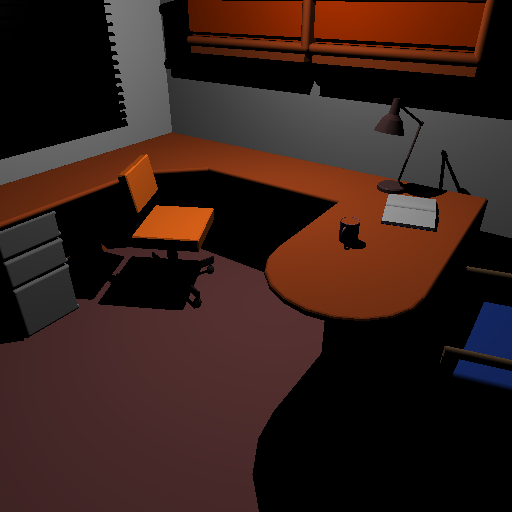
\includegraphics[width=4.0cm]{Images/Office_Preview}
        \captionof{figure}{\textsc{Office}}
    \end{minipage}
    \begin{minipage}{0.725\linewidth}
        \centering
        \fontencoding{T1}
        \fontseries{m}
        \fontshape{sc}
        \fontsize{8}{10}
        \selectfont
        \begin{tabular}[h]{l|rrr}
            \multicolumn{1}{c|}{\textsc{Office}} & \textsc{Level 3} & \textsc{Level 2} & \textsc{Level 1}\\
            \hline
            \emph{RAH Algorithm} & & \\
            \hline
            \quad \# Sh Intersections  & 17863536	& 131228368	& 202025920	\\
            \quad \# Sh Misses            & 1459990	& 105975128	& 186409563	\\
            \quad \# Sh Hits              & 16403546	& 25253240	& 15616357	\\
            \hline
            \emph{Our Algorithm} & & \\
            \hline
            \quad \# Sh Intersections  & 4108164    & 31864128	& 85755984	\\
            \quad \# Sh Misses         & 125148		& 21144630	& 76679022	\\
            \quad \# Sh Hits           & 3983016	& 10719498	& 9076962	\\
        \end{tabular}
        \label{table:office-d8-n3-results}
        \captionof{table}{\textsc{Office} Division 8 Depth 3 Test Results.}
    \end{minipage}
\end{figure}

\subsubsection{Cornell}

% Cornel Discussion

Comparing our algorithm with the RAH algorithm we can see that our algorithm computes 26,47\% less intersections than RAH on this scene. 91,17\% less than a brute force approach (see Table~\ref{table:cornell-d8-n3-results} and Table~\ref{table:results-d8-n3}).

% Cornell Table and Figure

\begin{figure}[!htb]
    \begin{minipage}{0.25\linewidth}
        \centering
        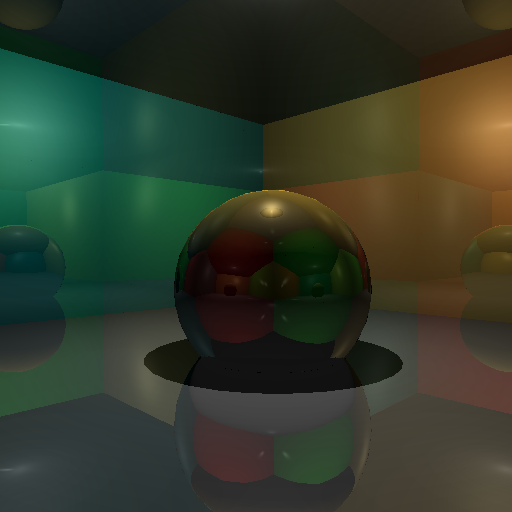
\includegraphics[width=4.0cm]{Images/Cornell_Preview}
        \captionof{figure}{\textsc{Cornell}}
    \end{minipage}
    \begin{minipage}{0.725\linewidth}
        \centering
        \fontencoding{T1}
        \fontseries{m}
        \fontshape{sc}
        \fontsize{8}{10}
        \selectfont
        \begin{tabular}[h]{l|rrr}
            \multicolumn{1}{c|}{\textsc{Office}} & \textsc{Level 3} & \textsc{Level 2} & \textsc{Level 1}\\
            \hline
            \emph{RAH Algorithm} & & \\
            \hline
            \quad \# Sh Intersections   & 374616 & 2617976 & 5156880    \\
            \quad \# Sh Misses             & 47369	 & 1973366 & 3606077    \\
            \quad \# Sh Hits               & 327247 & 644610  & 1550803    \\
            & & \\
            \quad \# Re Intersections   & 811008 & 6477632 & 17802296   \\
            \quad \# Re Misses             & 1304	 & 4252345 & 14311812   \\
            \quad \# Re Hits               & 809704 & 2225287 & 3490484    \\
            \hline
            \emph{Our Algorithm} & & \\
            \hline
            \quad \# Sh Intersections   & 181656 & 807208  & 2366280	\\
            \quad \# Sh Misses          & 80755	 & 511423  & 991955		\\
            \quad \# Sh Hits            & 100901 & 295785  & 1374325	\\
            & & \\
            \quad \# Re Intersections   & 614052 & 4143408 & 10278344	\\
            \quad \# Re Misses             & 96126	 & 2858615 & 6992777	\\
            \quad \# Re Hits               & 517926 & 1284793 & 3285567	\\            
        \end{tabular}
        \label{table:cornell-d8-n3-results}
        \captionof{table}{\textsc{Cornell} Division 8 Depth 3 Test Results.}
    \end{minipage}
\end{figure}

\subsubsection{Sponza}

% Sponza Discussion

Comparing our algorithm with the RAH algorithm we can see that our algorithm computes 35,86\% less intersections than RAH on this scene. 97,62\% less than a brute force approach (see Table~\ref{table:sponza-d8-n3-results} and Table~\ref{table:results-d8-n3}).

% Sponza Table and Figure

\begin{figure}[!htb]
    \begin{minipage}{0.25\linewidth}
        \centering
        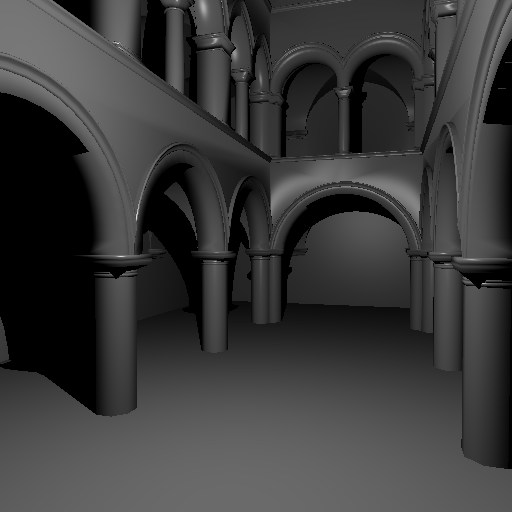
\includegraphics[width=4.0cm]{Images/Sponza_Preview}
        \captionof{figure}{\textsc{Sponza}}
    \end{minipage}
    \begin{minipage}{0.725\linewidth}
        \centering
        \fontencoding{T1}
        \fontseries{m}
        \fontshape{sc}
        \fontsize{8}{10}
        \selectfont
        \begin{tabular}[h]{l|rrr}
            \multicolumn{1}{c|}{\textsc{Office}} & \textsc{Level 3} & \textsc{Level 2} & \textsc{Level 1}\\
            \hline
            \emph{RAH Algorithm} & & \\
            \hline
            \quad \# Sh Intersections  & 33357900   & 214961944	& 261132816	\\
            \quad \# Sh Misses            & 6487657	& 182320342	& 248455163	\\
            \quad \# Sh Hits              & 26870243	& 32641602	& 12677653	\\
            & & \\
            \hline
            \emph{Our Algorithm} & & \\
            \hline
            \quad \# Sh Intersections   & 33357900	& 23359968	& 61887672	\\
            \quad \# Sh Misses          & 30437904	& 15624009	& 53120871	\\
            \quad \# Sh Hits            & 2919996	& 7735959	& 8766801	\\
        \end{tabular}
        \label{table:sponza-d8-n3-results}
        \captionof{table}{\textsc{Sponza} Division 8 Depth 3 Test Results.}
    \end{minipage}
\end{figure}

\subsection{Hierarchy Traversal Discussion - Subdivision 8 Depth 3}

% Comparison Table

\begin{table}[!htb]
    \begin{center}
    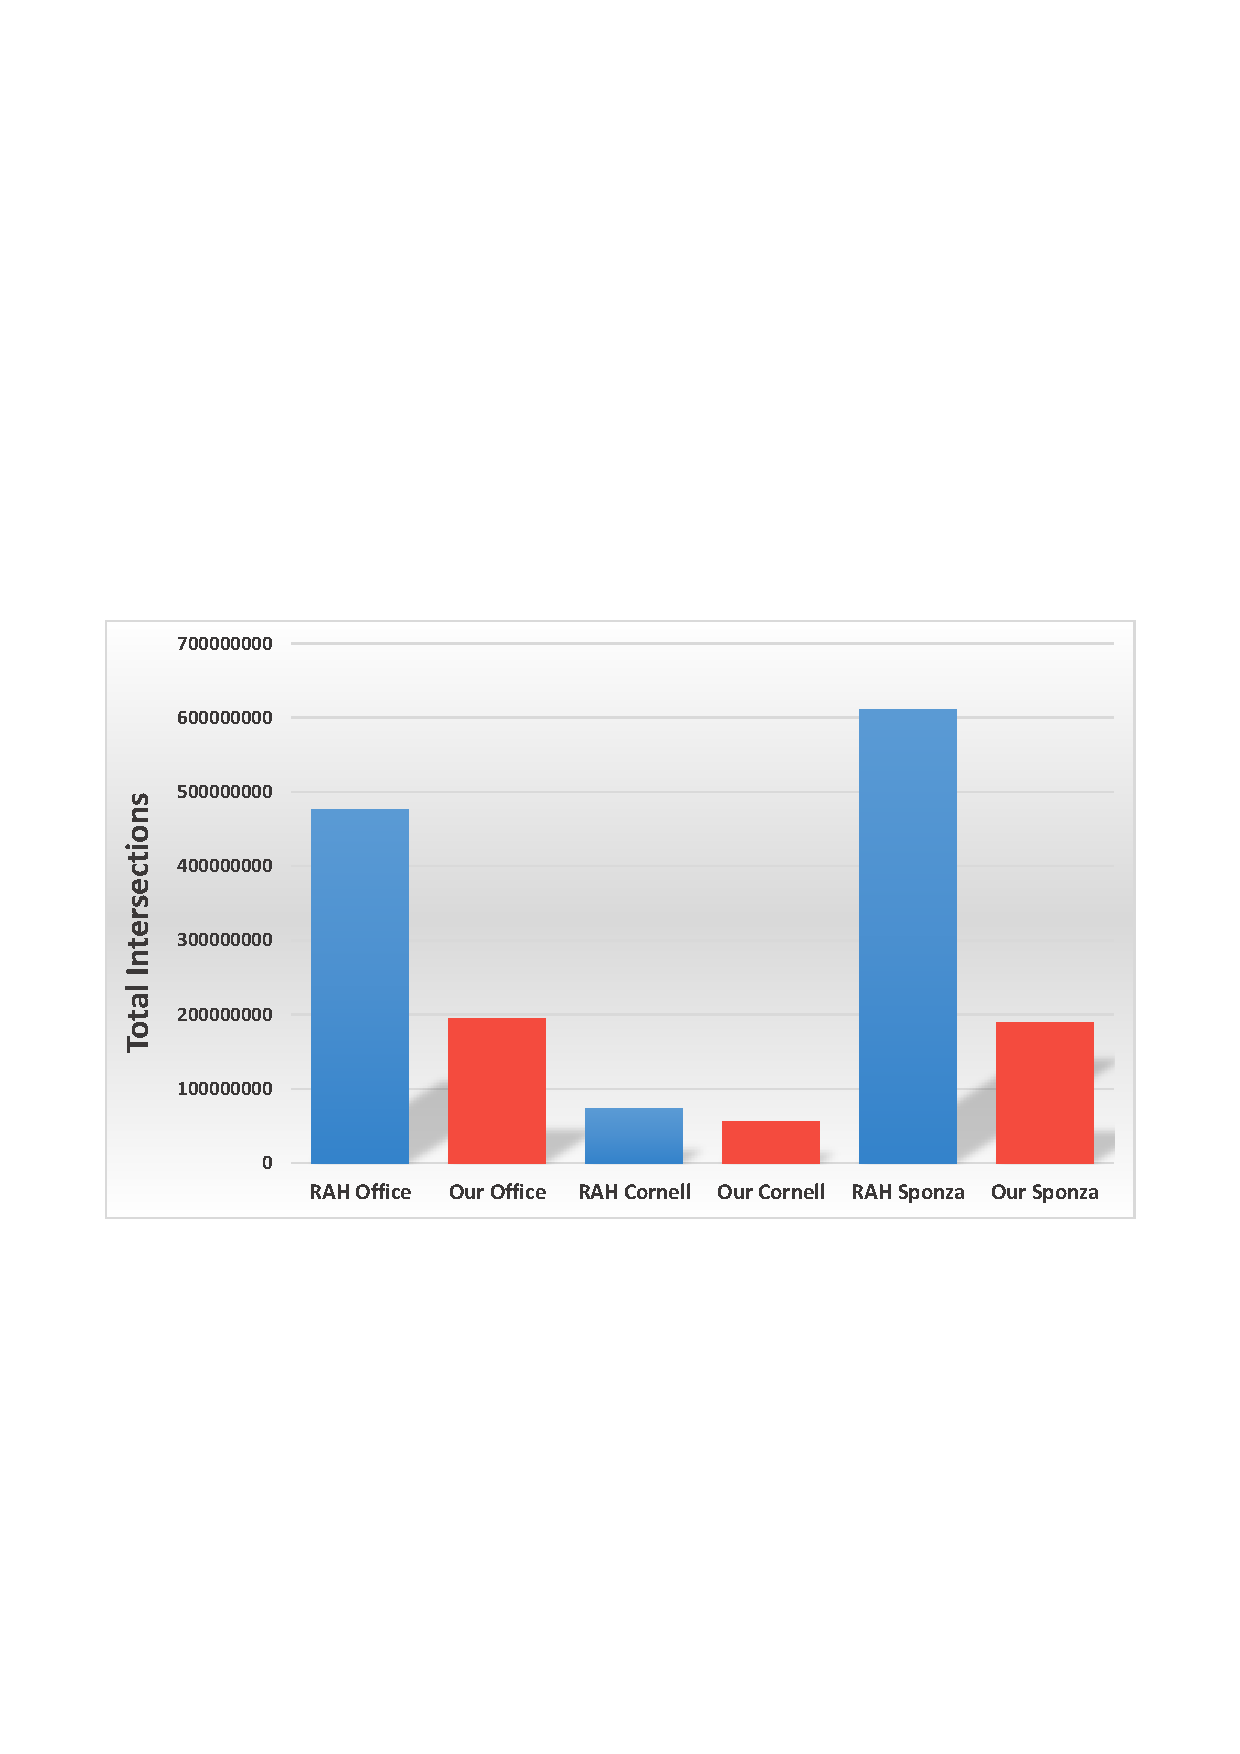
\includegraphics[width=0.85\textwidth]{Images/Chart_N8_D3}
    \vskip 2em
    \fontencoding{T1}
    \fontseries{m}
    \fontshape{sc}
    \fontsize{8}{10}
    \selectfont
    \begin{tabular}{l|rrrrrr}
    & \multicolumn{2}{c}{\textsc{Office}} & \multicolumn{2}{c}{\textsc{Cornell}} & \multicolumn{2}{c}{\textsc{Sponza}} \\
    \textsc{Algorithm} & \textsc{Total \# isect} & \textsc{Relative \%} & \textsc{Total \# isect} & \textsc{Relative \%} & \textsc{Total \# isect} & \textsc{Relative \%} \\
        \hline
        \emph{Brute Force}     & 9133132168         & 100\%           & 606911976         & 100\%           & 17058578850        & 100\% \\
        \emph{RAH Algorithm}   & 476048680		    & 5.21\%          & 73570704		  & 12.12\%         & 632408864			 & 3.58\% \\
        \emph{Our Algorithm}   & \textbf{194343972} & \textbf{2.13\%} & \textbf{55670084} & \textbf{9.17\%} & \textbf{188739948} & \textbf{1.11\%} \\
    \end{tabular}
    \end{center}
    \caption{\label{table:results-d8-n3}
    \small\textsc{Office} (251546 shadow rays), \textsc{Cornell} (242015 shadow \& 524288 reflection rays), \textsc{Sponza} (256713 shadow rays)  rendering performance using node subdivision 8 and hierarchy depth 3.}
\end{table}

\begin{figure}[!htb]
    \begin{center}
    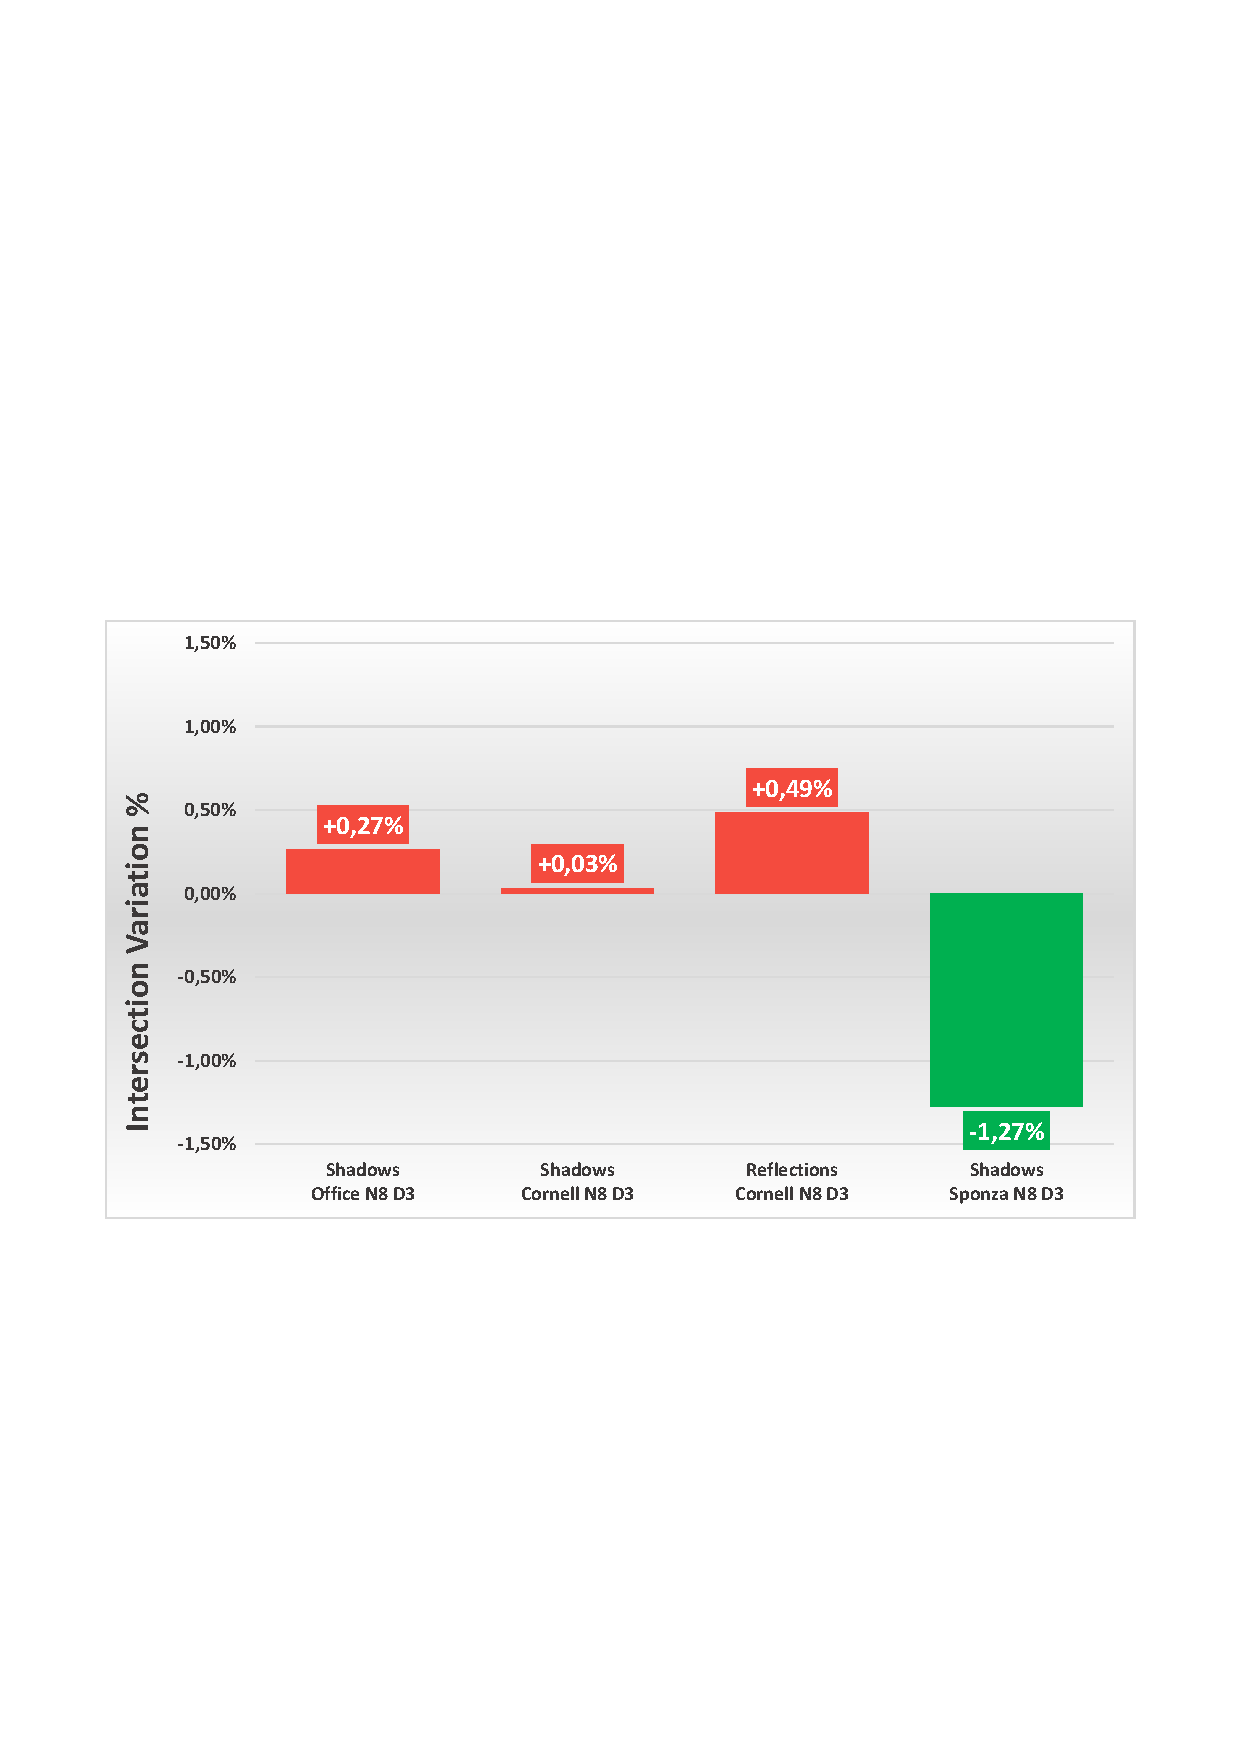
\includegraphics[width=0.85\textwidth]{Images/Chart_Comparison_N8_D2_N8_D3}
    \label{fig:comparison-results-d8-n2-d8-n3}
    \caption{Configuration Comparison between Node Subdivision 8 with Hierarchy Depth 2 and Node Subdivision 8 with Hierarchy Depth 3.}
    \end{center}
\end{figure}

For this set of tests we used a node subdivision of 8 and a hierarchy depth of 3. This means that every node in the upper levels of the hierarchy consists of 8 nodes in the level directly below. We compared this configuration with the baseline configuration of node subdivision of 8 and hierarchy depth of 2.

\subsubsection{Office}

Like our previous tests results, this configuration manages to outperform the RAH algorithm once more (see Table~\ref{table:office-d8-n3-results}). We compute 59,18\% less intersections than RAH on this scene and 97,87\% less than a brute force approach. There is however an increase in the number of intersection tests compared to the baseline configuration. The baseline configuration computes 1.86\% of the brute force intersection total while this configuration computes 2.13\%, a difference of 0.27\%, which amounts to about 13\% more intersection tests (see Figure~\ref{fig:comparison-results-d8-n2-d8-n3}).

\subsubsection{Cornell}

For the Cornell scene we compute 24,33\% less intersections overall (shadow and reflection rays combined) than the RAH algorithm and 90,83\% less than the brute force approach (see Table~\ref{table:cornell-d8-n3-results}). Like in the Office scene there is an increase in the intersection total, from 7.45\% to 7.48\% for shadow rays and from 9.46\% to 9.95\% for reflection rays (see Figure~\ref{fig:comparison-results-d8-n2-d8-n3}).

\subsubsection{Sponza}

In the Sponza scene we compute 69,10\% less intersection tests than RAH and 98,89\% than the brute force approach (see Table~\ref{table:sponza-d8-n3-results}). Unlike previous scenes however the number of intersection tests was reduced from 2.38\% to 1.11\% (see Figure~\ref{fig:comparison-results-d8-n2-d8-n3}). This can be explained by the bigger depth of the hierarchy. Since there aren't any object bounding spheres for this scene every single triangle is tested for intersections with the hierarchy's top nodes. This means that most of these triangles are culled at the first step of the traversal, leading to an overall lower number of intersection tests when compared with a hierarchy with lower depth. There should however be a break point after which the increase in depth will yield no further benefits.

%%%%%%%%%%%%%%%%%%%%%%%%%%%%%%%%%%%%%%%%%%%%%%%%%%%%%%%%%%%%%%%%%%%%%%%%%%%%%%%%%%%%%%%%%%%%%%%%%%%%%%%%%%%%%%%%%%%%%%%%%%%%%%%%%%

\pagebreak
\subsection{Hierarchy Traversal Results - Subdivision 8 Depth 4}

\subsubsection{Office}

% Office Discussion

Comparing our algorithm with the RAH algorithm we can see that our algorithm computes 39,18\% less intersections than RAH on this scene. 97,87\% less than a brute force approach (see Table~\ref{table:office-d8-n4-results} and Table~\ref{table:results-d8-n4}).

% Office Table and Figure
    
\begin{figure}[!htb]
    \begin{minipage}{0.25\linewidth}
        \centering
        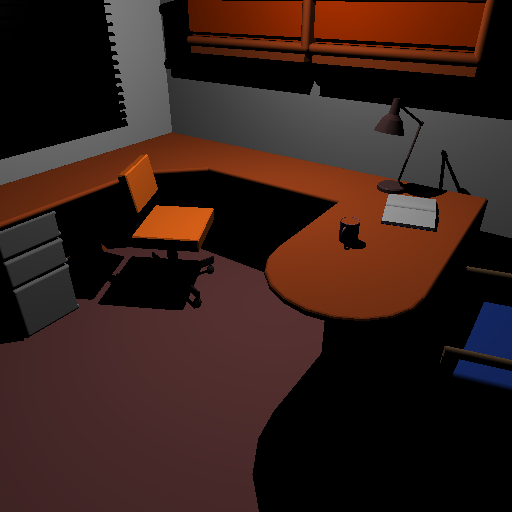
\includegraphics[width=4.0cm]{Images/Office_Preview}
        \captionof{figure}{\textsc{Office}}
    \end{minipage}
    \begin{minipage}{0.725\linewidth}
        \centering
        \fontencoding{T1}
        \fontseries{m}
        \fontshape{sc}
        \fontsize{8}{10}
        \selectfont
        \begin{tabular}[h]{l|rrrr}
            \multicolumn{1}{c|}{\textsc{Office}} & \textsc{Level 4} & \textsc{Level 3} & \textsc{Level 2} & \textsc{Level 1}\\
            \hline
            \emph{RAH Algorithm} & & \\
            \hline
            \quad \# Sh Intersections  & 2251096    & 16736728	& 131228368	& 202025920	\\
            \quad \# Sh Misses         & 159005		& 333182	& 105975128	& 186409563	\\
            \quad \# Sh Hits           & 2092091	& 16403546	& 25253240	& 15616357	\\
            \hline
            \emph{Our Algorithm} & & \\
            \hline
            \quad \# Sh Intersections  & 1398238	& 11068016	& 31896768	& 85725152	\\
            \quad \# Sh Misses         & 14736		& 7080920	& 21181124	& 76679166	\\
            \quad \# Sh Hits           & 1383502	& 3987096	& 10715644	& 9045986	\\
        \end{tabular}
        \label{table:office-d8-n4-results}
        \captionof{table}{\textsc{Office} Division 8 Depth 4 Test Results.}
    \end{minipage}
\end{figure}

\subsubsection{Cornell}

% Cornel Discussion

Comparing our algorithm with the RAH algorithm we can see that our algorithm computes 26,47\% less intersections than RAH on this scene. 91,17\% less than a brute force approach (see Table~\ref{table:cornell-d8-n4-results} and Table~\ref{table:results-d8-n4}).

% Cornell Table and Figure

\begin{figure}[!htb]
    \begin{minipage}{0.25\linewidth}
        \centering
        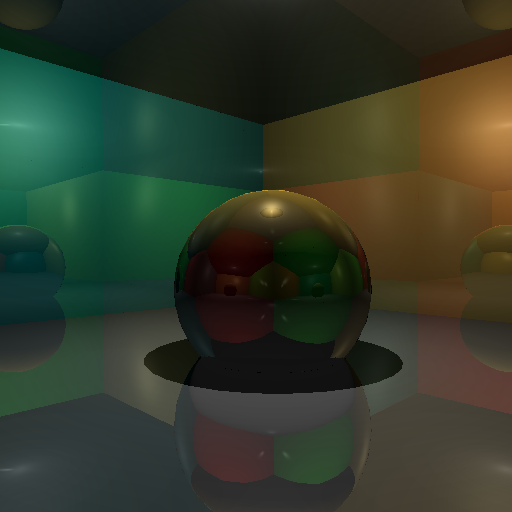
\includegraphics[width=4.0cm]{Images/Cornell_Preview}
        \captionof{figure}{\textsc{Cornell}}
    \end{minipage}
    \begin{minipage}{0.725\linewidth}
        \centering
        \fontencoding{T1}
        \fontseries{m}
        \fontshape{sc}
        \fontsize{8}{10}
        \selectfont
        \begin{tabular}[h]{l|rrrr}
            \multicolumn{1}{c|}{\textsc{Office}} & \textsc{Level 4} & \textsc{Level 3} & \textsc{Level 2} & \textsc{Level 1}\\
            \hline
            \emph{RAH Algorithm} & & \\
            \hline
            \quad \# Sh Intersections   & 47520	    & 335304    & 2617944	& 5150792   \\
            \quad \# Sh Misses          & 5607	    & 8061		& 1974095	& 3600819	\\
            \quad \# Sh Hits            & 41913	    & 327243	& 643849	& 1549973	\\
            & & \\
            \quad \# Re Intersections   & 101376    & 809824	& 6477632   & 17802296  \\
            \quad \# Re Misses          & 148	    & 120	    & 4252345	& 14311812	\\
            \quad \# Re Hits            & 101228	& 809704	& 1284793	& 3490484	\\
            \hline
            \emph{Our Algorithm} & & \\
            \hline
            \quad \# Sh Intersections   & 35280	    & 235248	& 807920	& 2358088	\\
            \quad \# Sh Misses          & 5874		& 134258	& 513159	& 991955	\\
            \quad \# Sh Hits            & 29406	    & 100990    & 294761	& 1366133	\\
            & & \\
            \quad \# Re Intersections   & 101376	& 809808	& 4144632	& 10278344	\\
            \quad \# Re Misses          & 150		& 291729	& 2859839	& 6992777	\\
            \quad \# Re Hits            & 101226	& 518079	& 1284793	& 3285567	\\            
        \end{tabular}
        \label{table:cornell-d8-n4-results}
        \captionof{table}{\textsc{Cornell} Division 8 Depth 4 Test Results.}
    \end{minipage}
\end{figure}

\subsubsection{Sponza}

% Sponza Discussion

Comparing our algorithm with the RAH algorithm we can see that our algorithm computes 35,86\% less intersections than RAH on this scene. 97,62\% less than a brute force approach (see Table~\ref{table:cornell-d8-n4-results} and Table~\ref{table:results-d8-n4}).

% Sponza Table and Figure

\begin{figure}[!htb]
    \begin{minipage}{0.25\linewidth}
        \centering
        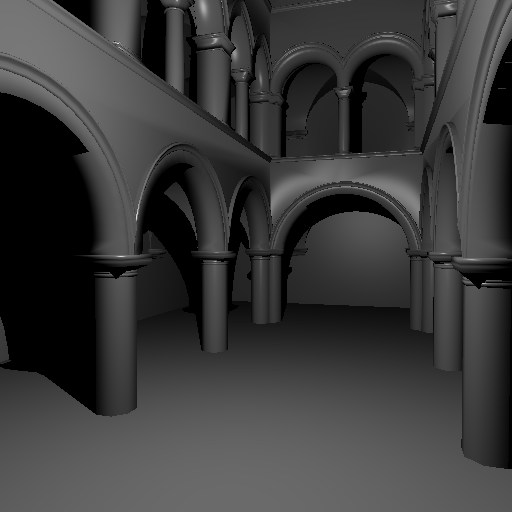
\includegraphics[width=4.0cm]{Images/Sponza_Preview}
        \captionof{figure}{\textsc{Sponza}}
    \end{minipage}
    \begin{minipage}{0.725\linewidth}
        \centering
        \fontencoding{T1}
        \fontseries{m}
        \fontshape{sc}
        \fontsize{8}{10}
        \selectfont
        \begin{tabular}[h]{l|rrrr}
            \multicolumn{1}{c|}{\textsc{Office}} & \textsc{Level 4} & \textsc{Level 3} & \textsc{Level 2} & \textsc{Level 1}\\
            \hline
            \emph{RAH Algorithm} & & \\
            \hline
            \quad \# Sh Intersections   & 4186350	& 27458720  & 214961944	& 261132816	\\
            \quad \# Sh Misses          & 754010	& 588477	& 182320342	& 248455163	\\
            \quad \# Sh Hits            & 3432340	& 26870243	& 32641602	& 12677653	\\
            & & \\
            \hline
            \emph{Our Algorithm} & & \\
            \hline
            \quad \# Sh Intersections   & 4186350	& 12578168	& 23263056	& 61112376	\\
            \quad \# Sh Misses          & 2614079	& 9670286	& 15624009	& 53120871	\\
            \quad \# Sh Hits            & 1572271	& 2907882	& 7639047	& 7991505	\\
        \end{tabular}
        \label{table:sponza-d8-n4-results}
        \captionof{table}{\textsc{Sponza} Division 8 Depth 4 Test Results.}
    \end{minipage}
\end{figure}

\subsection{Hierarchy Traversal Discussion - Subdivision 8 Depth 4}

% Comparison Table

\begin{table}[!htb]
    \begin{center}
    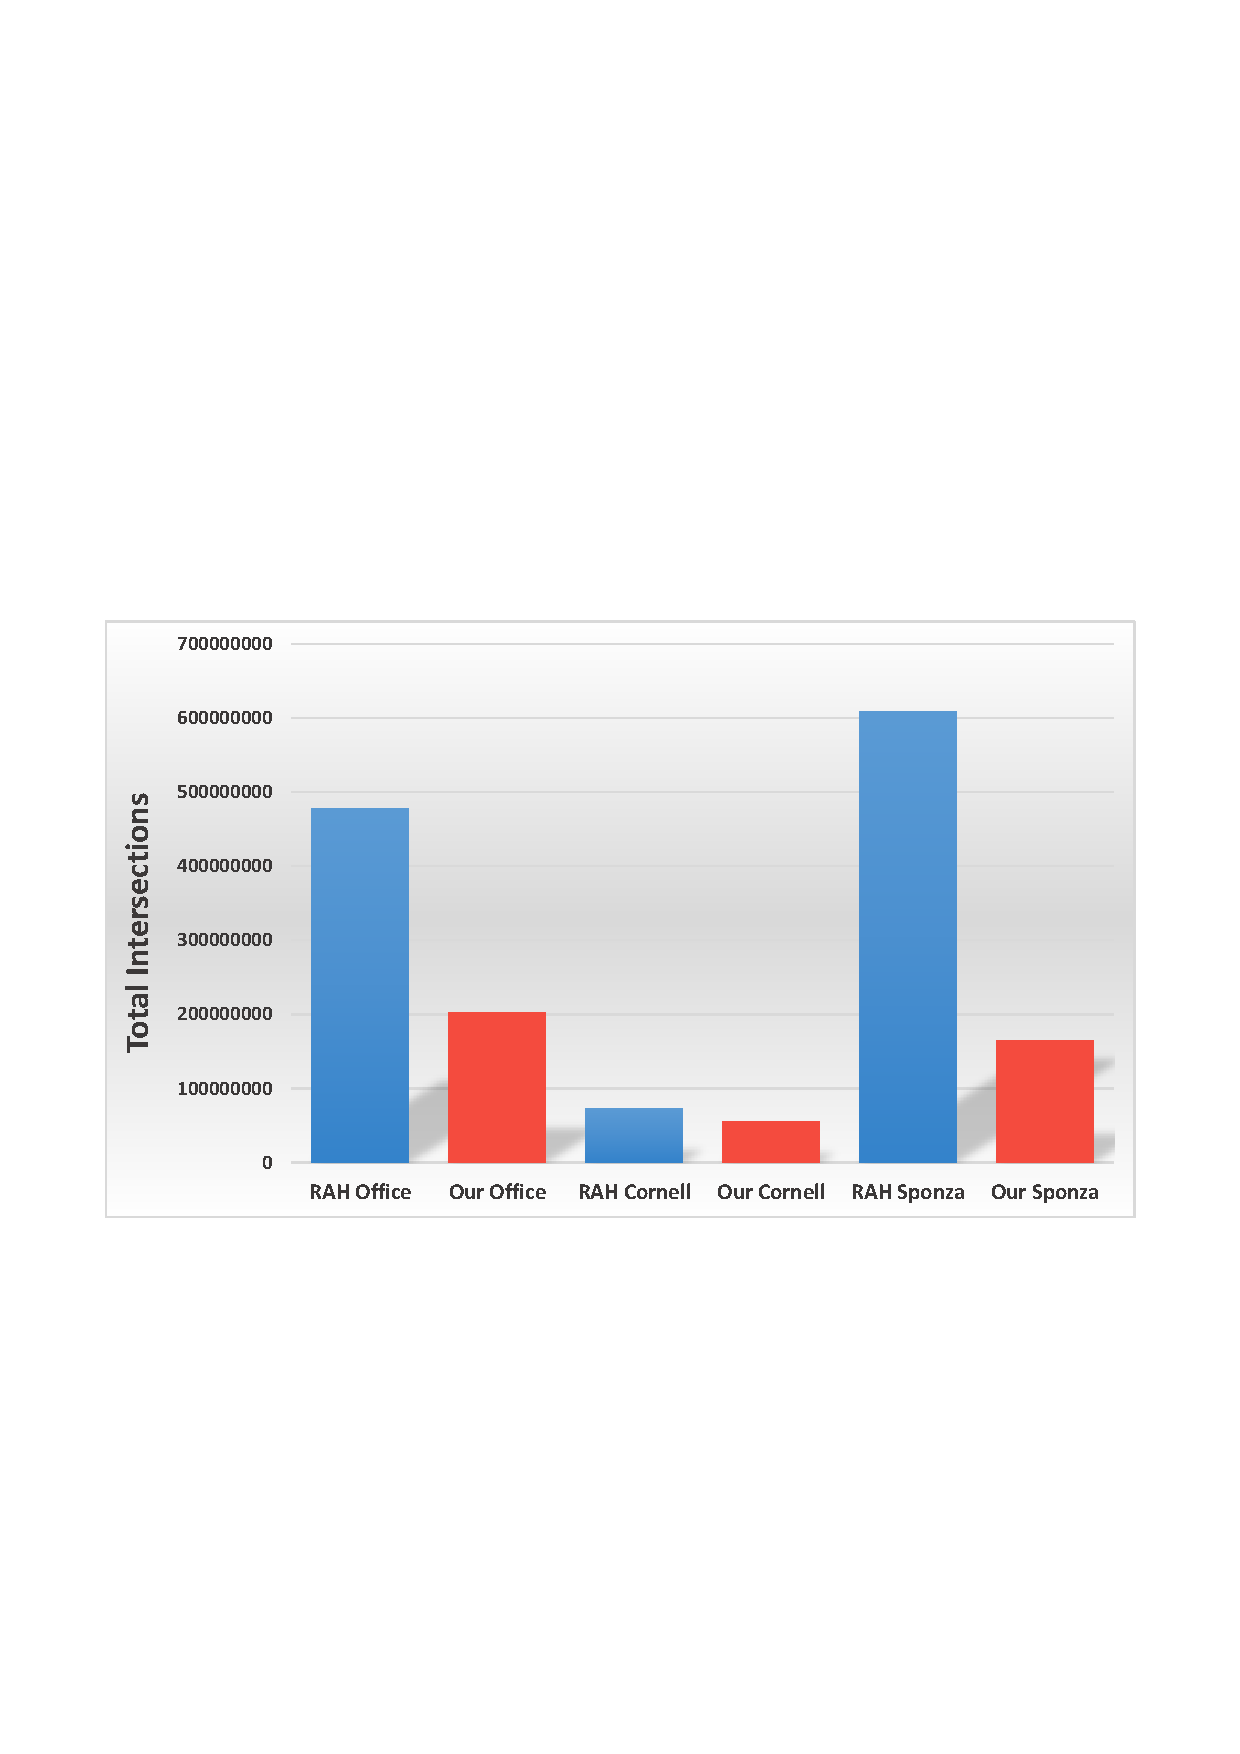
\includegraphics[width=0.85\textwidth]{Images/Chart_N8_D4}
    \vskip 2em
    \fontencoding{T1}
    \fontseries{m}
    \fontshape{sc}
    \fontsize{8}{10}
    \selectfont
    \begin{tabular}{l|rrrrrr}
    & \multicolumn{2}{c}{\textsc{Office}} & \multicolumn{2}{c}{\textsc{Cornell}} & \multicolumn{2}{c}{\textsc{Sponza}} \\
    \textsc{Algorithm} & \textsc{Total \# isect} & \textsc{Relative \%} & \textsc{Total \# isect} & \textsc{Relative \%} & \textsc{Total \# isect} & \textsc{Relative \%} \\
        \hline
        \emph{Brute Force}     & 9133132168         & 100\%           & 606911976         & 100\%           & 17058578850        & 100\% \\
        \emph{RAH Algorithm}   & 477172968			& 5.22\%          & 73666344		  & 12.14\%         & 609161054			 & 3.57\% \\
        \emph{Our Algorithm}   & \textbf{202456062} & \textbf{2.22\%} & \textbf{55984296} & \textbf{9.22\%} & \textbf{165071990} & \textbf{0.97\%} \\
    \end{tabular}
    \end{center}
    \caption{\label{table:results-d8-n4}
    \small\textsc{Office} (251546 shadow rays), \textsc{Cornell} (242015 shadow \& 524288 reflection rays), \textsc{Sponza} (256713 shadow rays) rendering performance using node subdivision 8 and hierarchy depth 4.}
\end{table}

\begin{figure}[!htb]
    \begin{center}
    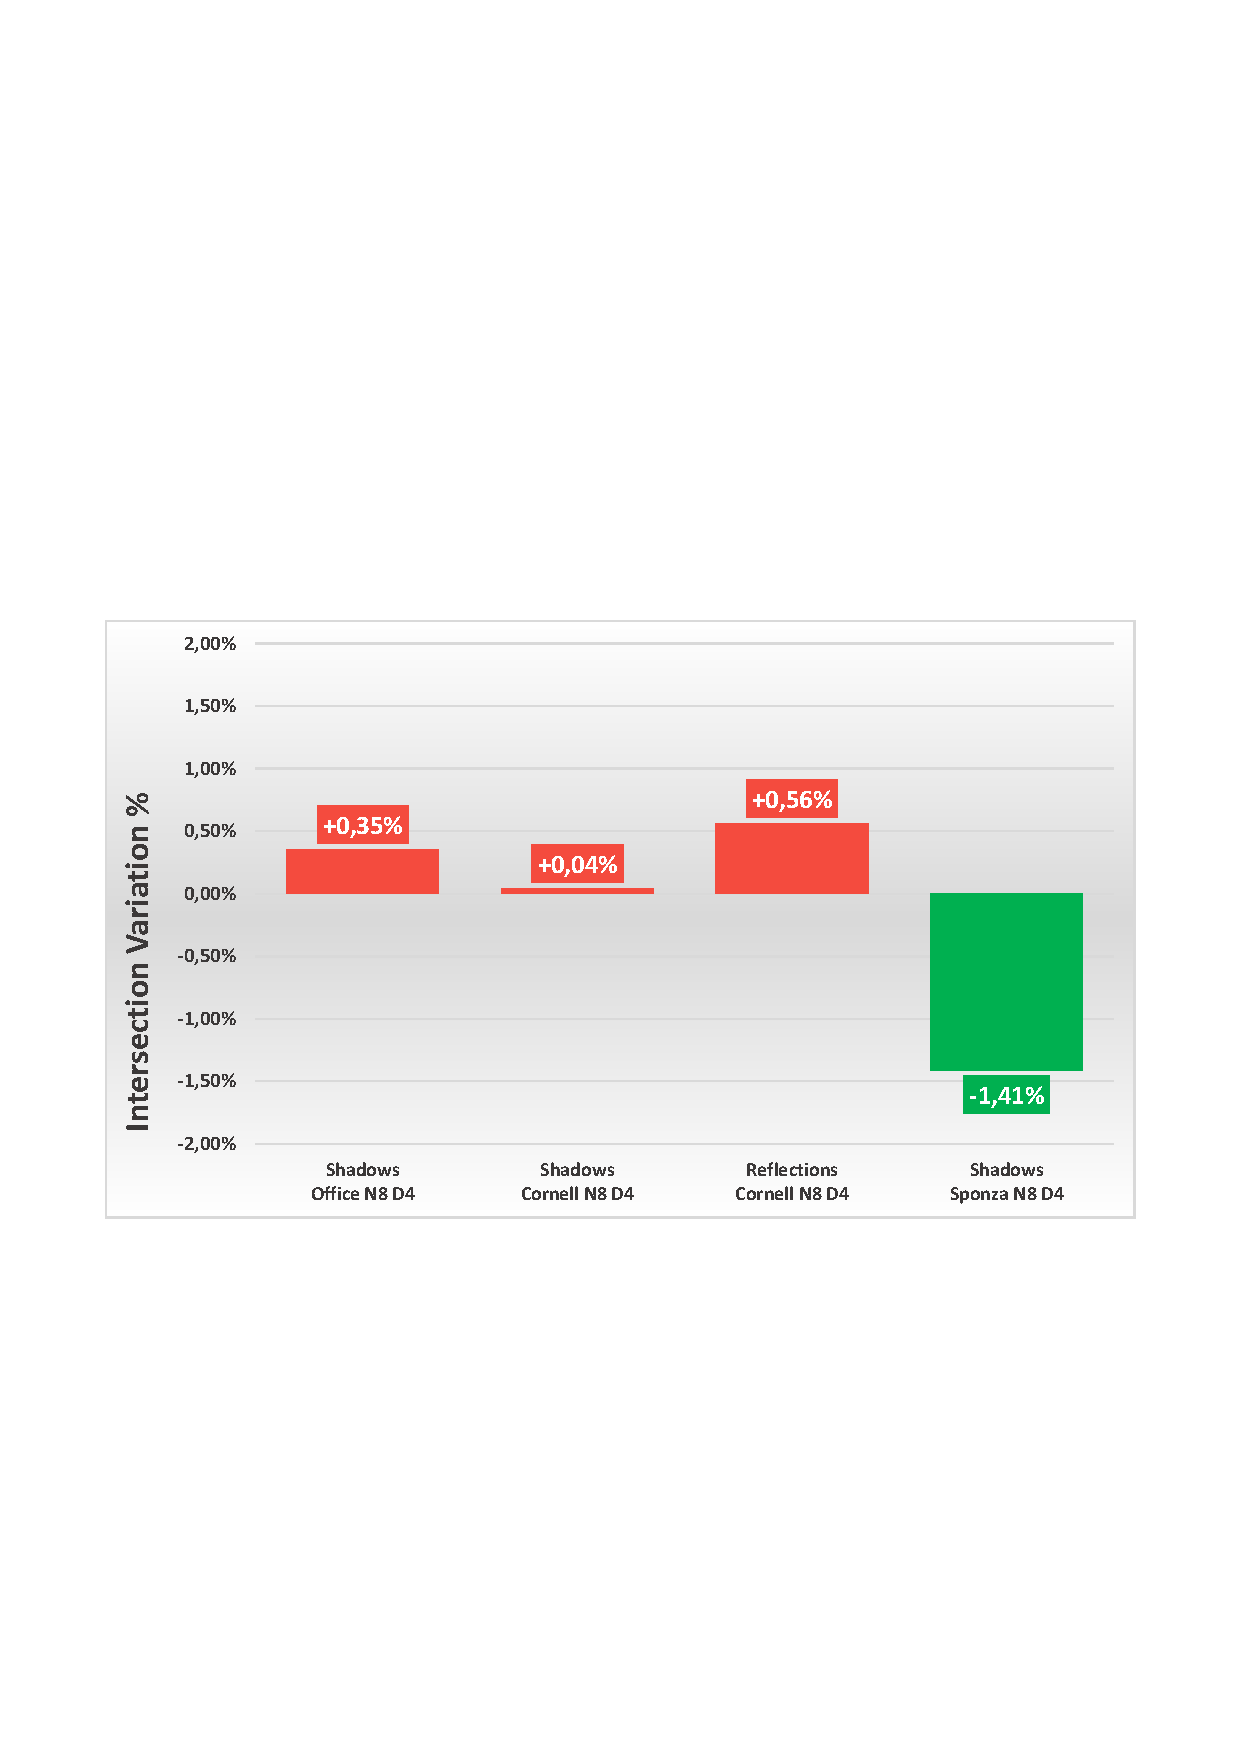
\includegraphics[width=0.70\textwidth]{Images/Chart_Comparison_N8_D2_N8_D4}
    \label{fig:comparison-results-d8-n2-d8-n4}
    \caption{Configuration Comparison between Node Subdivision 8 with Hierarchy Depth 2 and Node Subdivision 8 with Hierarchy Depth 4.}
    \end{center}
\end{figure}

For this set of tests we used a node subdivision of 8 and a hierarchy depth of 4. This means that every node in the upper levels of the hierarchy consists of 8 nodes in the level directly below. We compared this configuration with the baseline configuration of node subdivision of 8 and hierarchy depth of 2.

\subsubsection{Office}

Like our previous tests results, this configuration manages to outperform the RAH algorithm once more (see Table~\ref{table:office-d8-n4-results}). We compute 57,57\% less intersections than RAH on this scene and 97,78\% less than a brute force approach. The tendency for an increase in the intersection total shown in the previous comparison continued for this test. There is an increase from 1.86\% to 2,22\% of the brute force intersection total (see Figure~\ref{fig:comparison-results-d8-n2-d8-n4}).

\subsubsection{Cornell}

For the Cornell scene we compute 24,00\% less intersections overall (shadow and reflection rays combined) than the RAH algorithm and 90,78\% less than the brute force approach (see Table~\ref{table:cornell-d8-n4-results}). Like in the Office scene the tendency for an increase in the intersection total remains as we increase the hierarchies depth. The percentage rose from 7.45\% to 7.49\% for shadow rays and from 9.46\% to 10.02\% for reflection rays (see Figure~\ref{fig:comparison-results-d8-n2-d8-n4}).

\subsubsection{Sponza}

In the Sponza scene we compute 72,90\% less intersection tests than RAH and 99,03\% than the brute force approach (see Table~\ref{table:sponza-d8-n4-results}). The number of intersection tests was reduced once again, going from 2.38\% to 0.97\% (see Figure~\ref{fig:comparison-results-d8-n2-d8-n4}). Our hypothesis remains consistent since as we increase the hierarchy's depth the number of overall intersections keeps dropping for this particular scene.

%%%%%%%%%%%%%%%%%%%%%%%%%%%%%%%%%%%%%%%%%%%%%%%%%%%%%%%%%%%%%%%%%%%%%%%%%%%%%%%%%%%%%%%%%%%%%%%%%%%%%%%%%%%%%%%%%%%%%%%%%%%%%%%%%%

\pagebreak
\subsection{Hierarchy Traversal Results - Subdivision 16 Depth 2}

\subsubsection{Office}

% Office Discussion

Comparing our algorithm with the RAH algorithm we can see that our algorithm computes 39,18\% less intersections than RAH on this scene. 97,87\% less than a brute force approach (see Table~\ref{table:office-d16-n2-results} and Table~\ref{table:results-d16-n2}).

% Office Table and Figure
    
\begin{figure}[!htb]
    \begin{minipage}{0.25\linewidth}
        \centering
        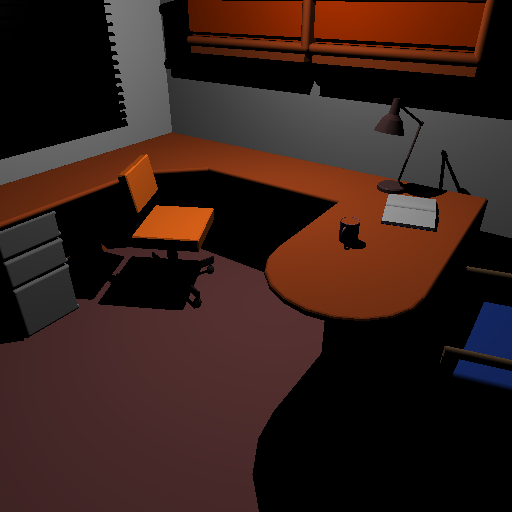
\includegraphics[width=4.0cm]{Images/Office_Preview}
        \captionof{figure}{\textsc{Office}}
    \end{minipage}
    \begin{minipage}{0.725\linewidth}
        \centering
        \fontencoding{T1}
        \fontseries{m}
        \fontshape{sc}
        \fontsize{8}{10}
        \selectfont
        \begin{tabular}[h]{l|rr}
            \multicolumn{1}{c|}{\textsc{Office}} & \textsc{Level 2} & \textsc{Level 1}\\
            \hline
            \emph{RAH Algorithm} & & \\
            \hline
            \quad \# Sh Intersections   & 35690764	& 412453440	\\
            \quad \# Sh Misses          & 9912424	& 398662535	\\
            \quad \# Sh Hits            & 25778340  & 13790905	\\
            \hline
            \emph{Our Algorithm} & & \\
            \hline
            \quad \# Sh Intersections  & 7724430    & 119385600	\\
            \quad \# Sh Misses         & 262830	    & 112687674	\\
            \quad \# Sh Hits           & 7461600	& 6697926	\\
        \end{tabular}
        \label{table:office-d16-n2-results}
        \captionof{table}{\textsc{Office} Division 16 Depth 2 Test Results.}
    \end{minipage}
\end{figure}

\subsubsection{Cornell}

% Cornel Discussion

Comparing our algorithm with the RAH algorithm we can see that our algorithm computes 26,47\% less intersections than RAH on this scene. 91,17\% less than a brute force approach (see Table~\ref{table:cornell-d16-n2-results} and Table~\ref{table:results-d16-n2}).

% Cornell Table and Figure

\begin{figure}[!htb]
    \begin{minipage}{0.25\linewidth}
        \centering
        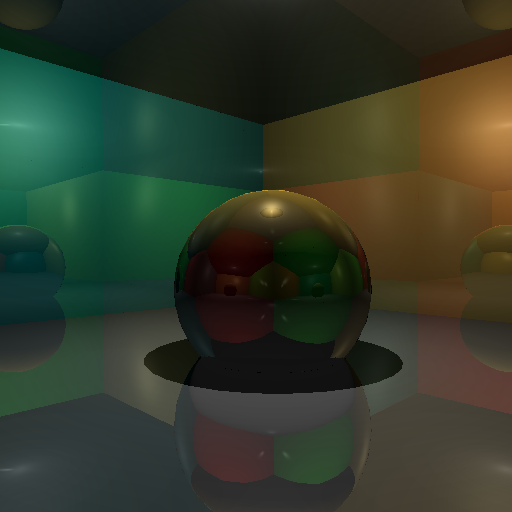
\includegraphics[width=4.0cm]{Images/Cornell_Preview}
        \captionof{figure}{\textsc{Cornell}}
    \end{minipage}
    \begin{minipage}{0.725\linewidth}
        \centering
        \fontencoding{T1}
        \fontseries{m}
        \fontshape{sc}
        \fontsize{8}{10}
        \selectfont
        \begin{tabular}[h]{l|rr}
            \multicolumn{1}{c|}{\textsc{Office}} & \textsc{Level 2} & \textsc{Level 1}\\
            \hline
            \emph{RAH Algorithm} & & \\
            \hline
            \quad \# Sh Intersections   & 749232    & 7732000	\\
            \quad \# Sh Misses          & 265982	& 6808346	\\
            \quad \# Sh Hits            & 483250	& 923654	\\
            & & \\
            \quad \# Re Intersections   & 1622016	& 23053680	\\
            \quad \# Re Misses          & 181161	& 20614507  \\
            \quad \# Re Hits            & 1440855	& 2439173   \\
            \hline
            \emph{Our Algorithm} & & \\
            \hline
            \quad \# Sh Intersections   & 343872    & 2571952	\\
            \quad \# Sh Misses          & 183125	& 1846363	\\
            \quad \# Sh Hits            & 160747	& 725589	\\
            & & \\
            \quad \# Re Intersections   & 983928	& 11460592	\\
            \quad \# Re Misses          & 267641	& 9368514	\\
            \quad \# Re Hits            & 716287	& 2092078	\\            
        \end{tabular}
        \label{table:cornell-d16-n2-results}
        \captionof{table}{\textsc{Cornell} Division 16 Depth 2 Test Results.}
    \end{minipage}
\end{figure}

\subsubsection{Sponza}

% Sponza Discussion

Comparing our algorithm with the RAH algorithm we can see that our algorithm computes 35,86\% less intersections than RAH on this scene. 97,62\% less than a brute force approach (see Table~\ref{table:sponza-d16-n2-results} and Table~\ref{table:results-d16-n2}).

% Sponza Table and Figure

\begin{figure}[!htb]
    \begin{minipage}{0.25\linewidth}
        \centering
        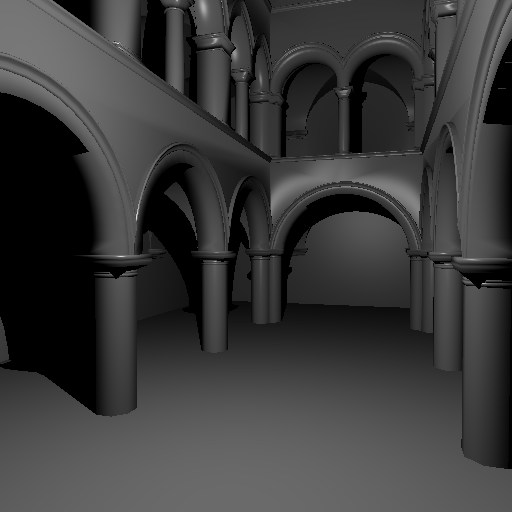
\includegraphics[width=4.0cm]{Images/Sponza_Preview}
        \captionof{figure}{\textsc{Sponza}}
    \end{minipage}
    \begin{minipage}{0.725\linewidth}
        \centering
        \fontencoding{T1}
        \fontseries{m}
        \fontshape{sc}
        \fontsize{8}{10}
        \selectfont
        \begin{tabular}[h]{l|rr}
            \multicolumn{1}{c|}{\textsc{Office}} & \textsc{Level 2} & \textsc{Level 1}\\
            \hline
            \emph{RAH Algorithm} & & \\
            \hline
            \quad \# Sh Intersections   & 66649350	& 554494192	\\
            \quad \# Sh Misses          & 31993463	& 544455870	\\
            \quad \# Sh Hits            & 34655887	& 10038322	\\
            & & \\
            \hline
            \emph{Our Algorithm} & & \\
            \hline
            \quad \# Sh Intersections   & 66649350	& 103145120	\\
            \quad \# Sh Misses          & 60202780	& 97483134	\\
            \quad \# Sh Hits            & 6446570	& 5661986	\\
        \end{tabular}
        \label{table:sponza-d16-n2-results}
        \captionof{table}{\textsc{Sponza} Division 16 Depth 2 Test Results.}
    \end{minipage}
\end{figure}

\subsection{Hierarchy Traversal Discussion - Subdivision 16 Depth 2}

% Comparison Table

\begin{table}[!htb]
    \begin{center}
    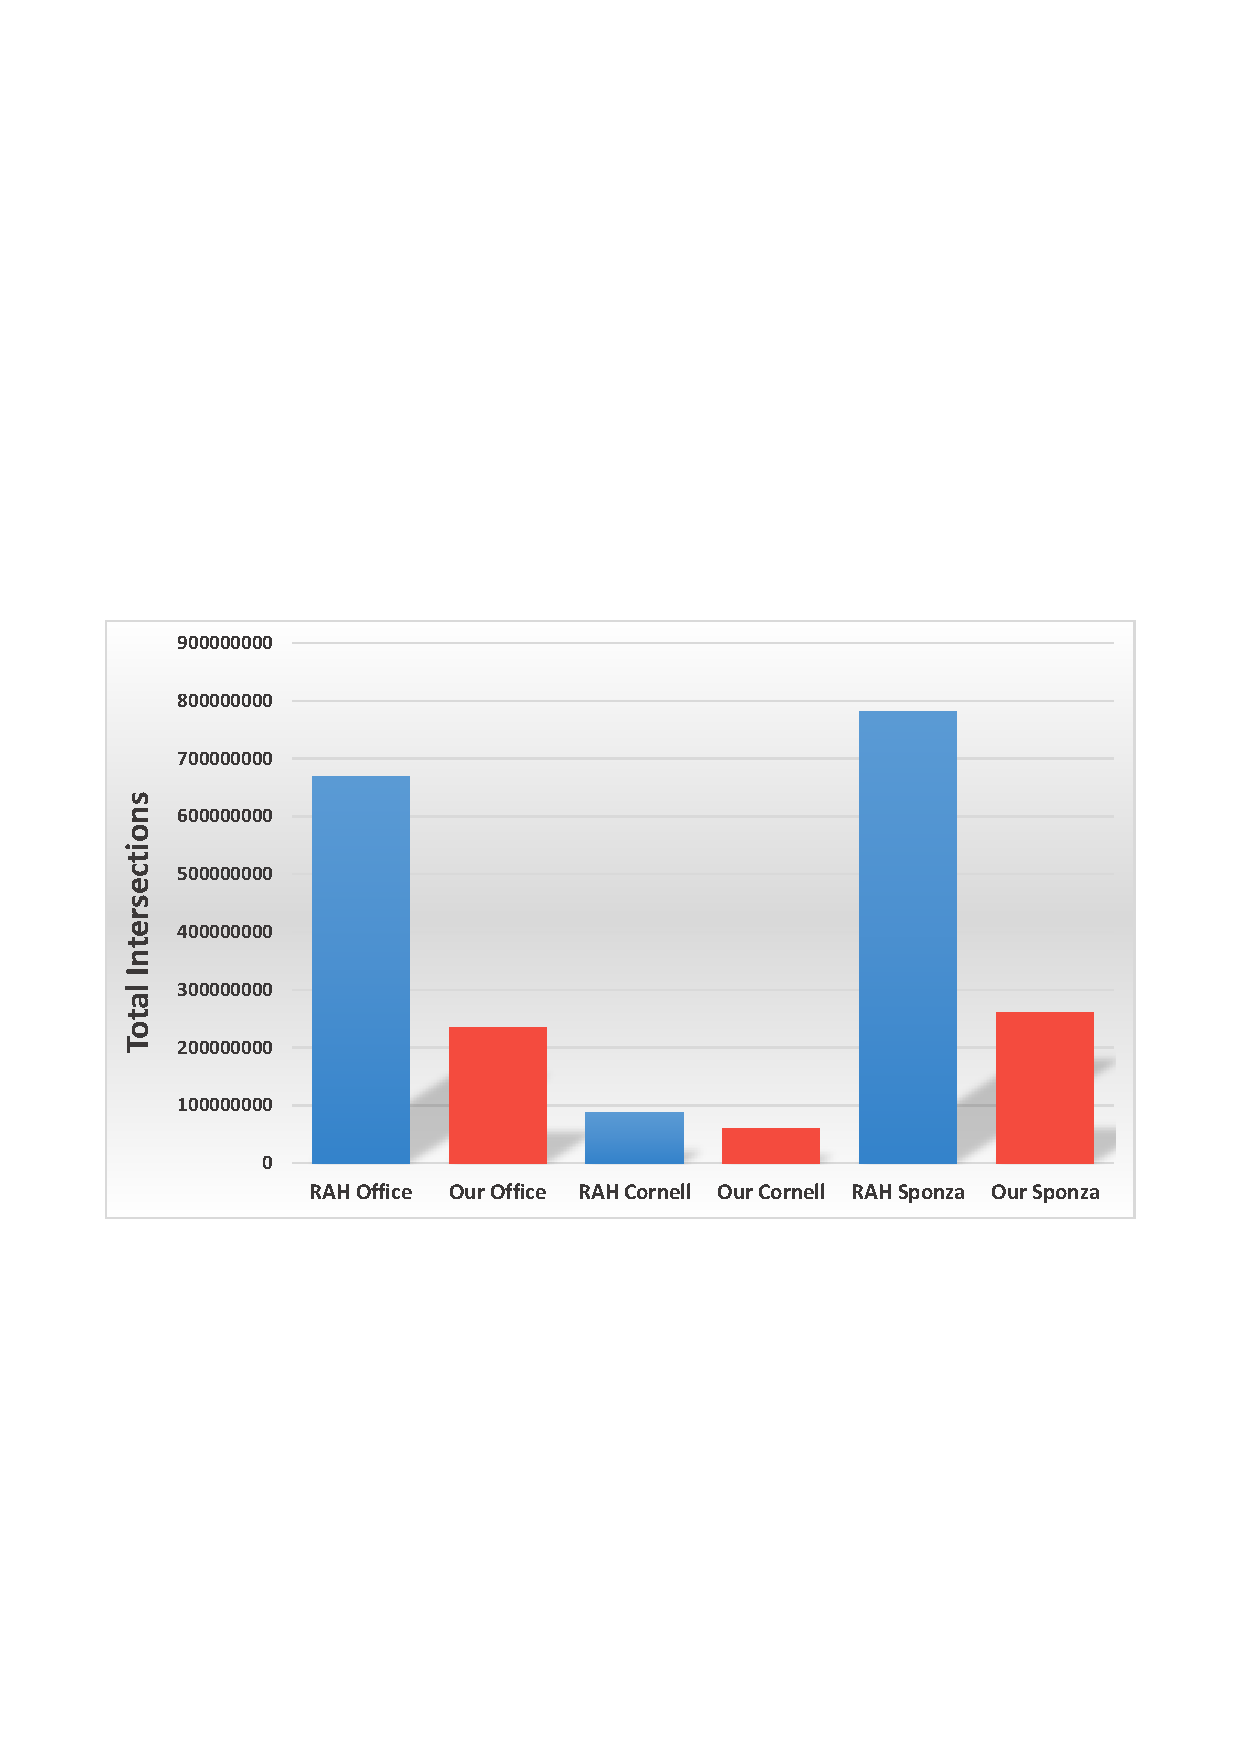
\includegraphics[width=0.85\textwidth]{Images/Chart_N16_D2}
    \vskip 2em
    \fontencoding{T1}
    \fontseries{m}
    \fontshape{sc}
    \fontsize{8}{10}
    \selectfont
    \begin{tabular}{l|rrrrrr}
    & \multicolumn{2}{c}{\textsc{Office}} & \multicolumn{2}{c}{\textsc{Cornell}} & \multicolumn{2}{c}{\textsc{Sponza}} \\
    \textsc{Algorithm} & \textsc{Total \# isect} & \textsc{Relative \%} & \textsc{Total \# isect} & \textsc{Relative \%} & \textsc{Total \# isect} & \textsc{Relative \%} \\
        \hline
        \emph{Brute Force}     & 9133132168         & 100\%           & 606911976           & 100\%           & 17058578850         & 100\% \\
        \emph{RAH Algorithm}   & 668798684		    & 7.32\%          & 86962160            & 14.33\%         & 781756694	        & 4.58\% \\
        \emph{Our Algorithm}   & \textbf{234276846} & \textbf{2.57\%} & \textbf{60443016}	& \textbf{9.96\%} & \textbf{260386246}  & \textbf{1.53\%} \\
    \end{tabular}
    \end{center}
    \caption{\label{table:results-d16-n2}
    \small\textsc{Office} (251546 shadow rays), \textsc{Cornell} (242015 shadow \& 524288 reflection rays), \textsc{Sponza} (256713 shadow rays) rendering performance using node subdivision 16 and hierarchy depth 2.}
\end{table}

\begin{figure}[!htb]
    \begin{center}
    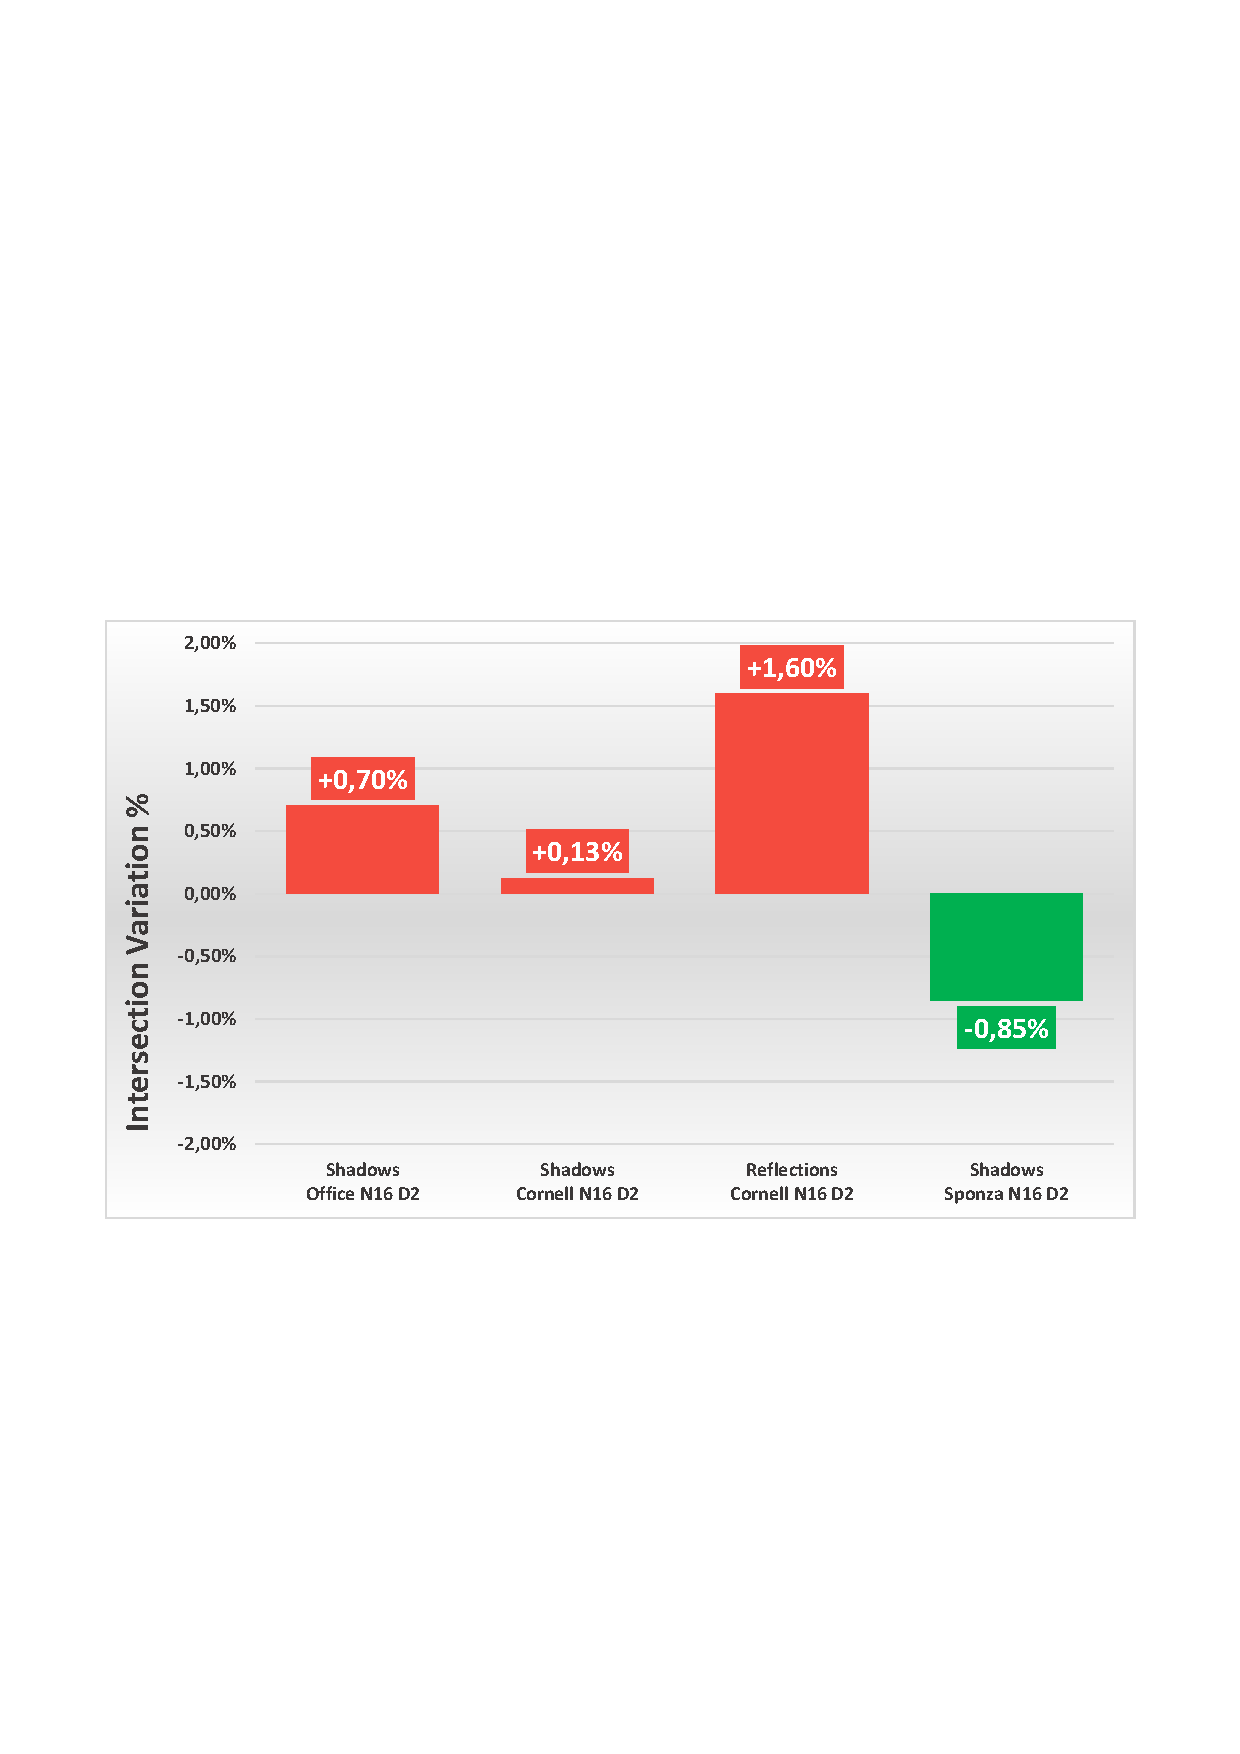
\includegraphics[width=0.70\textwidth]{Images/Chart_Comparison_N8_D2_N16_D2}
    \label{fig:comparison-results-d8-n2-d16-n2}
    \caption{Configuration Comparison between Node Subdivision 8 with Hierarchy Depth 2 and Node Subdivision 16 with Hierarchy Depth 2.}
    \end{center}
\end{figure}

For this set of tests we used a node subdivision of 16 and a hierarchy depth of 2. This means that every node in the upper levels of the hierarchy consists of 16 nodes in the level directly below. We compared this configuration with the baseline configuration of node subdivision of 8 and hierarchy depth of 2.

\subsubsection{Office}

With the new node subdivision this configuration still outperforms the RAH algorithm (see Table~\ref{table:office-d16-n2-results}). We compute 64,97\% less intersections than RAH on this scene and 97,43\% less than a brute force approach. These results are extremely close to the baseline configuration but there is still an increase of 0.70\% when compared to the baseline (from 1.86\% to 2.57\%) (see Figure~\ref{fig:comparison-results-d8-n2-d16-n2}).

\subsubsection{Cornell}

For the Cornell scene we compute 30,50\% less intersections overall (shadow and reflection rays combined) than the RAH algorithm and 90,04\% less than the brute force approach (see Table~\ref{table:cornell-d16-n2-results}). When we compare these results with the baseline configuration we get an increase of 0.13\%, from 7.45\% to 7.58\% for shadow rays and from 9.46\% to 11.06\% for reflection rays (see Figure~\ref{fig:comparison-results-d8-n2-d16-n2}).

\subsubsection{Sponza}

In the Sponza scene we compute 66,69\% less intersection tests than RAH and 98,47\% than the brute force approach (see Table~\ref{table:sponza-d16-n2-results}). The number of intersection tests was reduced once again, going from the baseline 2.38\% to 1.53\% (see Figure~\ref{fig:comparison-results-d8-n2-d16-n2}). This is slightly different from the previous cases but the explanation is very similar. Because every node consists of more rays the upper levels of the hierarchy discard even more test results for the traversal of the lower levels of the hierarchy, leading to the overall reduction in intersections.

%%%%%%%%%%%%%%%%%%%%%%%%%%%%%%%%%%%%%%%%%%%%%%%%%%%%%%%%%%%%%%%%%%%%%%%%%%%%%%%%%%%%%%%%%%%%%%%%%%%%%%%%%%%%%%%%%%%%%%%%%%%%%%%%%%

\pagebreak
\subsection{Hierarchy Traversal Results - Subdivision 16 Depth 3}

\subsubsection{Office}

% Office Discussion

Comparing our algorithm with the RAH algorithm we can see that our algorithm computes 39,18\% less intersections than RAH on this scene. 97,87\% less than a brute force approach (see Table~\ref{table:office-d16-n3-results} and Table~\ref{table:results-d16-n3}).

% Office Table and Figure
    
\begin{figure}[!htb]
    \begin{minipage}{0.25\linewidth}
        \centering
        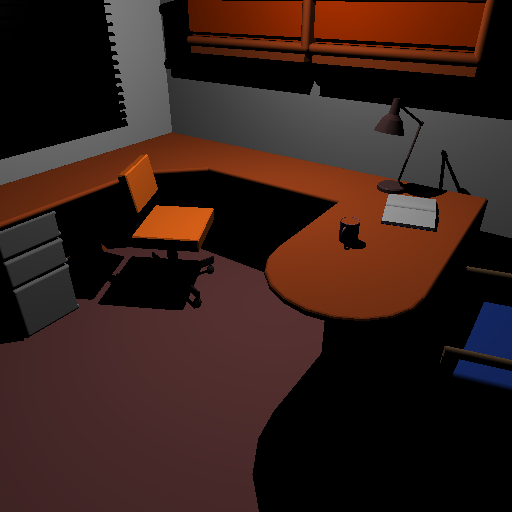
\includegraphics[width=4.0cm]{Images/Office_Preview}
        \captionof{figure}{\textsc{Office}}
    \end{minipage}
    \begin{minipage}{0.725\linewidth}
        \centering
        \fontencoding{T1}
        \fontseries{m}
        \fontshape{sc}
        \fontsize{8}{10}
        \selectfont
        \begin{tabular}[h]{l|rrr}
            \multicolumn{1}{c|}{\textsc{Office}} & \textsc{Level 3} & \textsc{Level 2} & \textsc{Level 1}\\
            \hline
            \emph{RAH Algorithm} & & \\
            \hline
            \quad \# Sh Intersections   & 2251096   & 36017536	& 412453440	\\
            \quad \# Sh Misses          & 0	        & 10239196	& 398662535	\\
            \quad \# Sh Hits            & 2251096	& 25778340  & 13790905	\\
            \hline
            \emph{Our Algorithm} & & \\
            \hline
            \quad \# Sh Intersections  & 1474802	& 23344000	& 119524928	\\
            \quad \# Sh Misses         & 15802		& 15873692	& 112848037	\\
            \quad \# Sh Hits           & 1459000	& 7470308	& 6676891	\\
        \end{tabular}
        \label{table:office-d16-n3-results}
        \captionof{table}{\textsc{Office} Division 16 Depth 3 Test Results.}
    \end{minipage}
\end{figure}

\subsubsection{Cornell}

% Cornel Discussion

Comparing our algorithm with the RAH algorithm we can see that our algorithm computes 26,47\% less intersections than RAH on this scene. 91,17\% less than a brute force approach (see Table~\ref{table:cornell-d16-n3-results} and Table~\ref{table:results-d16-n3}).

% Cornell Table and Figure

\begin{figure}[!htb]
    \begin{minipage}{0.25\linewidth}
        \centering
        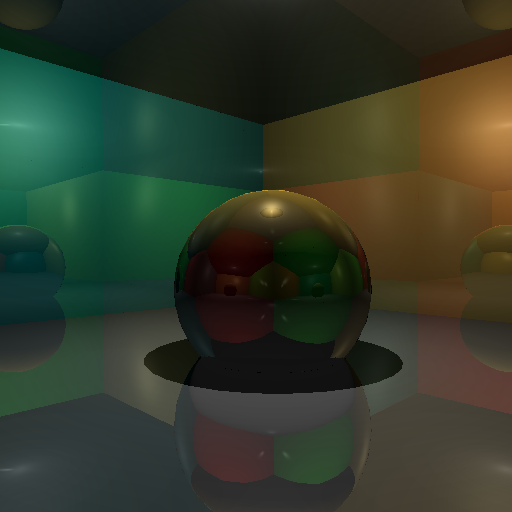
\includegraphics[width=4.0cm]{Images/Cornell_Preview}
        \captionof{figure}{\textsc{Cornell}}
    \end{minipage}
    \begin{minipage}{0.725\linewidth}
        \centering
        \fontencoding{T1}
        \fontseries{m}
        \fontshape{sc}
        \fontsize{8}{10}
        \selectfont
        \begin{tabular}[h]{l|rrr}
            \multicolumn{1}{c|}{\textsc{Office}} & \textsc{Level 3} & \textsc{Level 2} & \textsc{Level 1}\\
            \hline
            \emph{RAH Algorithm} & & \\
            \hline
            \quad \# Sh Intersections       & 47520     & 760128    & 7732000 \\
            \quad \# Sh Misses              & 12		& 276878    & 6808346 \\
            \quad \# Sh Hits                & 47508		& 483250	& 923654  \\
            & & \\
            \quad \# Re Intersections       & 101376	& 1622016	& 23053680  \\
            \quad \# Re Misses              & 0	        & 181161	& 20614507  \\
            \quad \# Re Hits                & 101376	& 1440855	& 2439173	\\
            \hline
            \emph{Our Algorithm} & & \\
            \hline
            \quad \# Sh Intersections       & 36720		& 498352	& 2577680	\\
            \quad \# Sh Misses              & 5573		& 337247	& 1856187	\\
            \quad \# Sh Hits                & 31147		& 161105	& 721493	\\
            & & \\
            \quad \# Re Intersections       & 101376	& 1620432	& 11466336	\\
            \quad \# Re Misses              & 99	    & 903786	& 9374256	\\
            \quad \# Re Hits                & 101277	& 716646	& 2092080	\\            
        \end{tabular}
        \label{table:cornell-d16-n3-results}
        \captionof{table}{\textsc{Cornell} Division 16 Depth 3 Test Results.}
    \end{minipage}
\end{figure}

\subsubsection{Sponza}

% Sponza Discussion

Comparing our algorithm with the RAH algorithm we can see that our algorithm computes 35,86\% less intersections than RAH on this scene. 97,62\% less than a brute force approach (see Table~\ref{table:sponza-d16-n3-results} and Table~\ref{table:results-d16-n3}).

% Sponza Table and Figure

\begin{figure}[!htb]
    \begin{minipage}{0.25\linewidth}
        \centering
        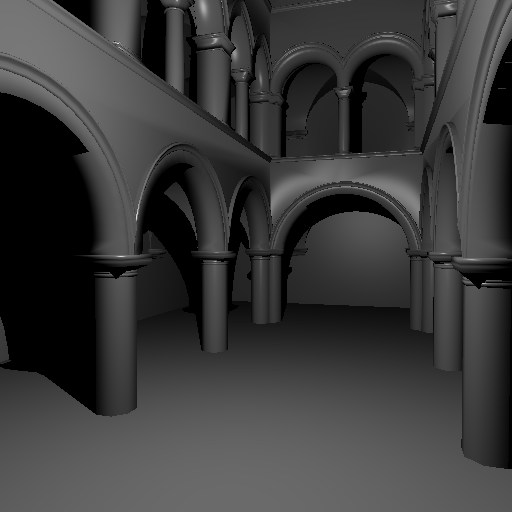
\includegraphics[width=4.0cm]{Images/Sponza_Preview}
        \captionof{figure}{\textsc{Sponza}}
    \end{minipage}
    \begin{minipage}{0.725\linewidth}
        \centering
        \fontencoding{T1}
        \fontseries{m}
        \fontshape{sc}
        \fontsize{8}{10}
        \selectfont
        \begin{tabular}[h]{l|rrr}
            \multicolumn{1}{c|}{\textsc{Office}} & \textsc{Level 3} & \textsc{Level 2} & \textsc{Level 1}\\
            \hline
            \emph{RAH Algorithm} & & \\
            \hline
            \quad \# Sh Intersections   & 4186350   & 66981600	& 554494192	\\
            \quad \# Sh Misses          & 0	        & 32325713	& 544455870	\\
            \quad \# Sh Hits            & 4186350	& 34655887	& 10038322	\\
            & & \\
            \hline
            \emph{Our Algorithm} & & \\
            \hline
            \quad \# Sh Intersections   & 4186350	& 29037376	& 102667568	\\
            \quad \# Sh Misses          & 2371514	& 22620653	& 97483134	\\
            \quad \# Sh Hits            & 1814836	& 6416723	& 5184434	\\
        \end{tabular}
        \label{table:sponza-d16-n3-results}
        \captionof{table}{\textsc{Sponza} Division 16 Depth 3 Test Results.}
    \end{minipage}
\end{figure}

\subsection{Hierarchy Traversal Discussion - Subdivision 16 Depth 3}

% Comparison Table

\begin{table}[!htb]
    \begin{center}
    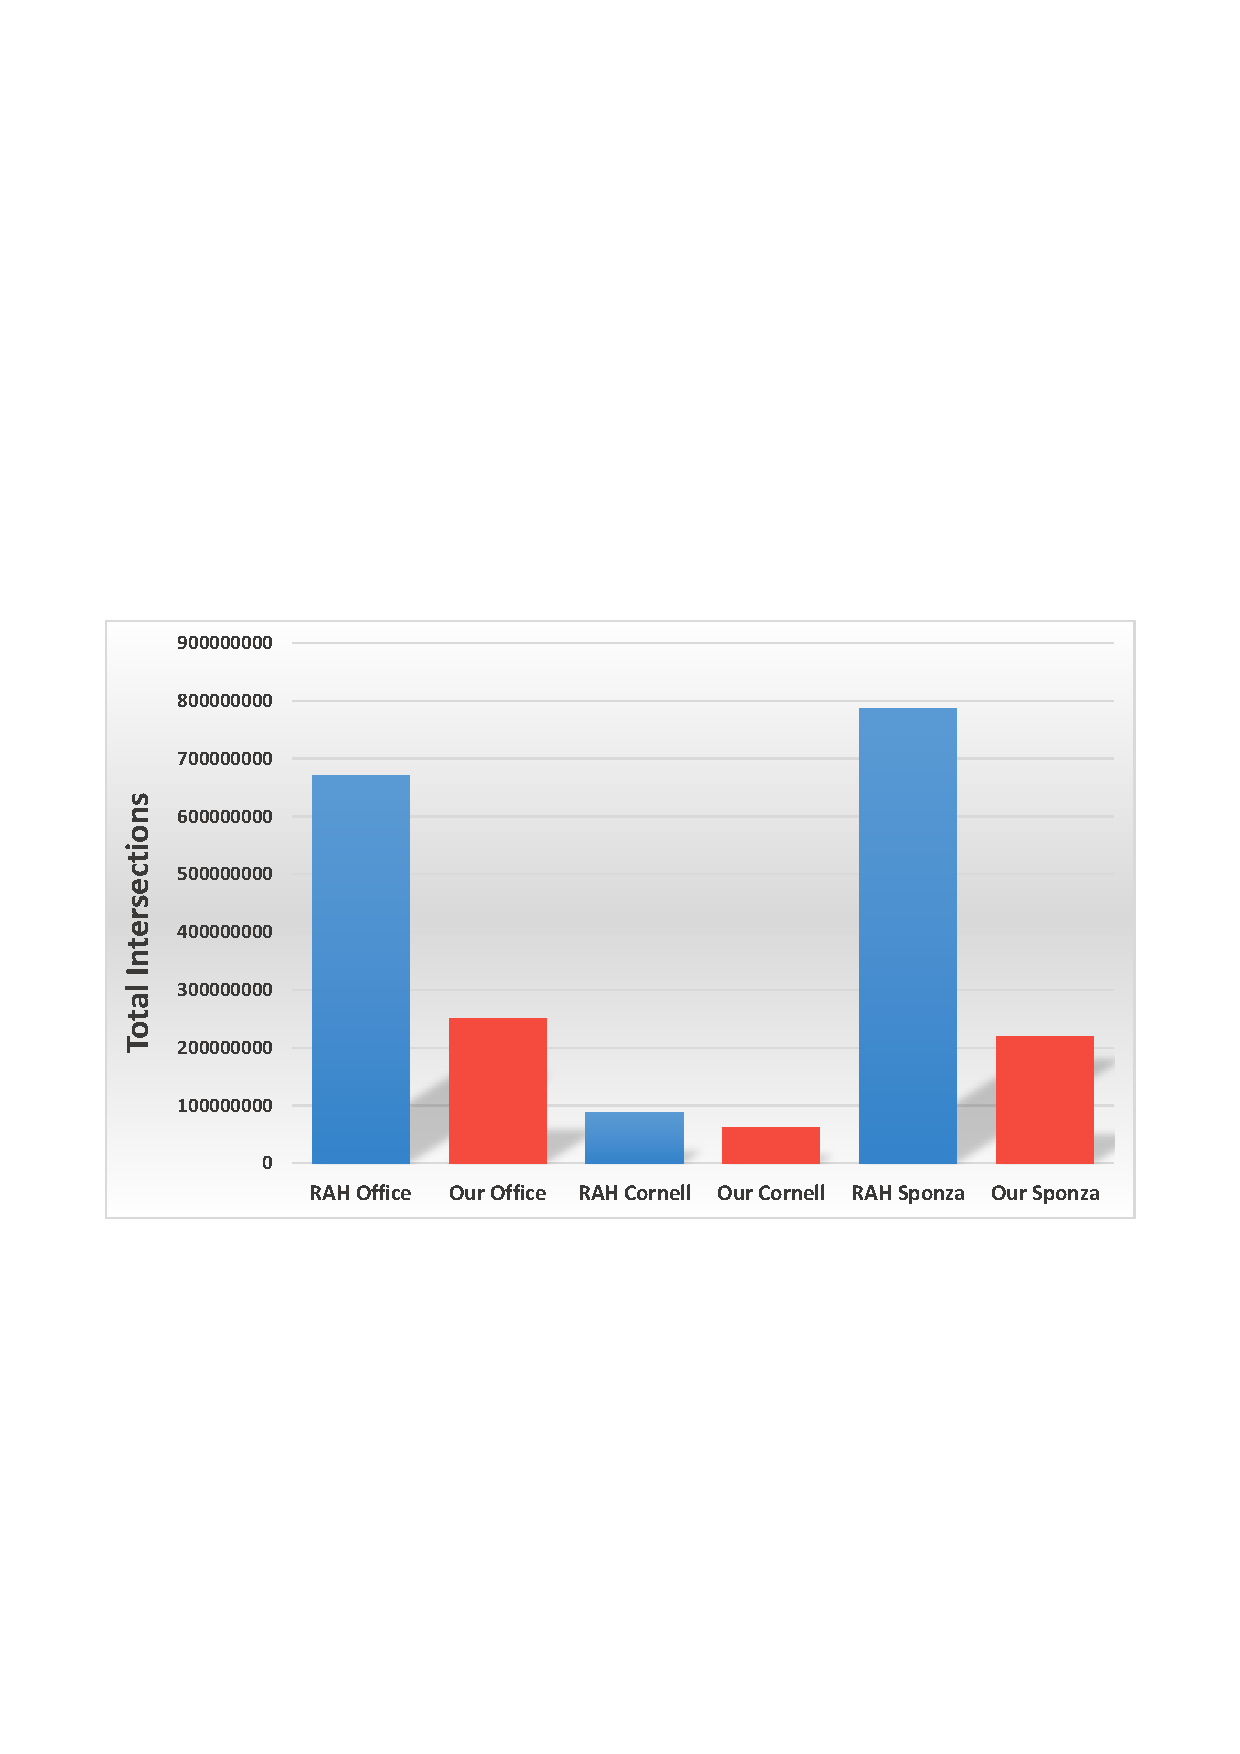
\includegraphics[width=0.85\textwidth]{Images/Chart_N16_D3}
    \vskip 2em
    \fontencoding{T1}
    \fontseries{m}
    \fontshape{sc}
    \fontsize{8}{10}
    \selectfont
    \begin{tabular}{l|rrrrrr}
    & \multicolumn{2}{c}{\textsc{Office}} & \multicolumn{2}{c}{\textsc{Cornell}} & \multicolumn{2}{c}{\textsc{Sponza}} \\
    \textsc{Algorithm} & \textsc{Total \# isect} & \textsc{Relative \%} & \textsc{Total \# isect} & \textsc{Relative \%} & \textsc{Total \# isect} & \textsc{Relative \%} \\
        \hline
        \emph{Brute Force}     & 9133132168         & 100\%           & 606911976         & 100\%           & 17058578850        & 100\% \\
        \emph{RAH Algorithm}   & 671376552			& 7.35\%          & 87121952		  & 14.35\%         & 786275294			 & 4.61\% \\
        \emph{Our Algorithm}   & \textbf{251173986} & \textbf{2.75\%} & \textbf{61318064} & \textbf{10.10\%} & \textbf{218842238} & \textbf{1.28\%} \\
    \end{tabular}
    \end{center}
    \caption{\label{table:results-d16-n3}
    \small\textsc{Office} (251546 shadow rays), \textsc{Cornell} (242015 shadow \& 524288 reflection rays), \textsc{Sponza} (256713 shadow rays) rendering performance using node subdivision 16 and hierarchy depth 3.}
\end{table}

\begin{figure}[!htb]
    \begin{center}
    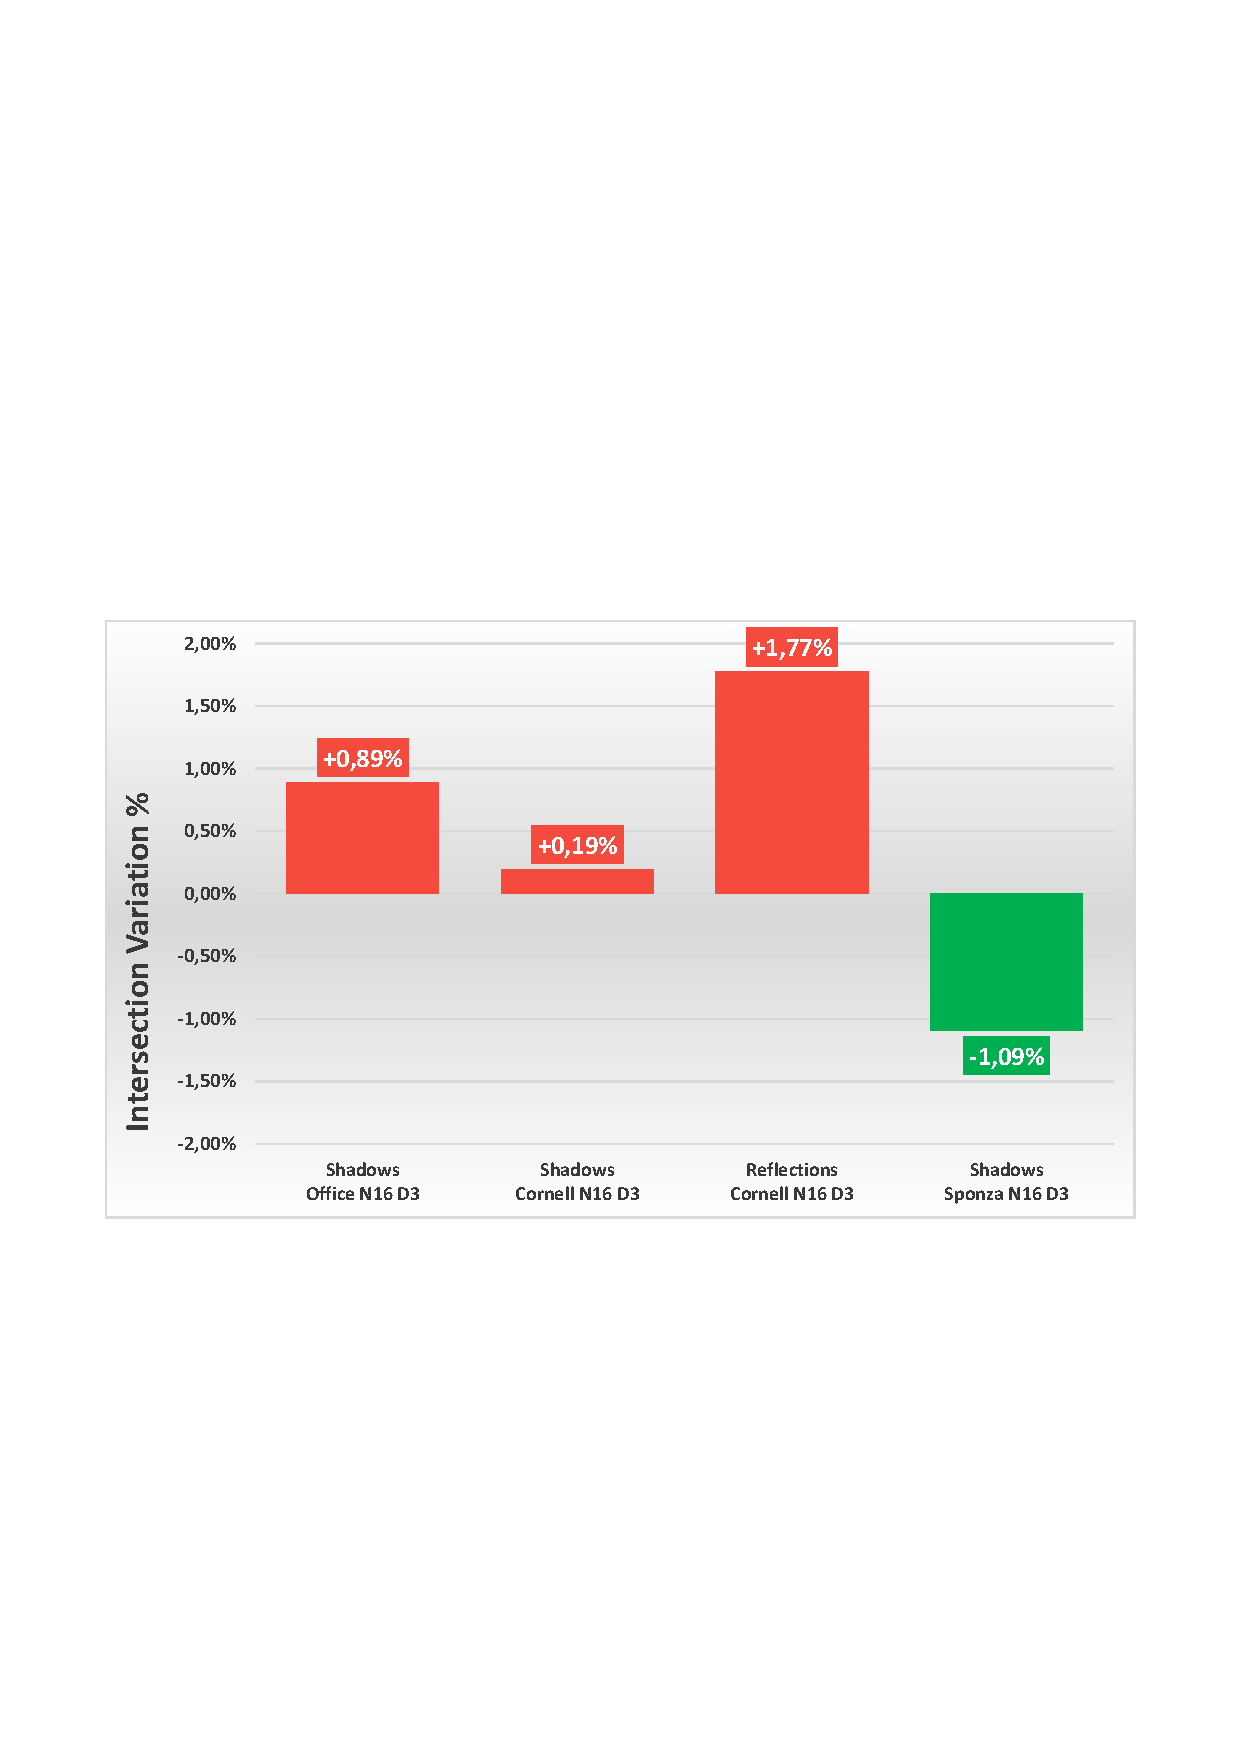
\includegraphics[width=0.70\textwidth]{Images/Chart_Comparison_N8_D2_N16_D3}
    \label{fig:comparison-results-d8-n2-d16-n3}
    \caption{Configuration Comparison between Node Subdivision 8 with Hierarchy Depth 2 and Node Subdivision 16 with Hierarchy Depth 3.}
    \end{center}
\end{figure}

For this set of tests we used a node subdivision of 16 and a hierarchy depth of 3. This means that every node in the upper levels of the hierarchy consists of 16 nodes in the level directly below. We compared this configuration with the baseline configuration of node subdivision of 8 and hierarchy depth of 2.

\subsubsection{Office}

Once more, increasing the depth of the hierarchy outperforms the RAH algorithm (see Table~\ref{table:office-d16-n3-results}). We compute 62.59\% less intersections than RAH on this scene and 97,25\% less than a brute force approach. There is an increase of 0.70\% when compared to the baseline (from 1.86\% to 2.75\%) (see Figure~\ref{fig:comparison-results-d8-n2-d16-n3}).

\subsubsection{Cornell}

For the Cornell scene we compute 29,62\% less intersections overall (shadow and reflection rays combined) than the RAH algorithm and 89,90\% less than the brute force approach (see Table~\ref{table:cornell-d16-n3-results}). When we compare these results with the baseline configuration we get an increase of 0.13\%, from 7.45\% to 7.65\% for shadow rays and from 9.46\% to 11.24\% for reflection rays (see Figure~\ref{fig:comparison-results-d8-n2-d16-n3}). This continues the trend seen in previous test results.

\subsubsection{Sponza}

In the Sponza scene we compute 72,17\% less intersection tests than RAH and 98,72\% than the brute force approach (see Table~\ref{table:sponza-d16-n3-results}). The number of intersection tests was reduced once again, going from the baseline 2.38\% to 1.28\% (see Figure~\ref{fig:comparison-results-d8-n2-d16-n3}). Since we increased the depth from the previous configuration it is natural that the trend for a decrease in intersection tests remains until we reach the break point.

%%%%%%%%%%%%%%%%%%%%%%%%%%%%%%%%%%%%%%%%%%%%%%%%%%%%%%%%%%%%%%%%%%%%%%%%%%%%%%%%%%%%%%%%%%%%%%%%%%%%%%%%%%%%%%%%%%%%%%%%%%%%%%%%%%

\pagebreak
\subsection{Hierarchy Traversal Results - Subdivision 16 Depth 4}

\subsubsection{Office}

% Office Discussion

Comparing our algorithm with the RAH algorithm we can see that our algorithm computes 39,18\% less intersections than RAH on this scene. 97,87\% less than a brute force approach (see Table~\ref{table:office-d16-n4-results} and Table~\ref{table:results-d16-n4}).

% Office Table and Figure
    
\begin{figure}[!htb]
    \begin{minipage}{0.25\linewidth}
        \centering
        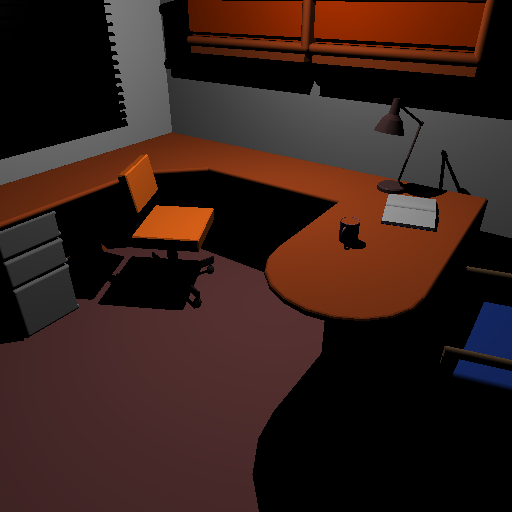
\includegraphics[width=4.0cm]{Images/Office_Preview}
        \captionof{figure}{\textsc{Office}}
    \end{minipage}
    \begin{minipage}{0.725\linewidth}
        \centering
        \fontencoding{T1}
        \fontseries{m}
        \fontshape{sc}
        \fontsize{8}{10}
        \selectfont
        \begin{tabular}[h]{l|rrrr}
            \multicolumn{1}{c|}{\textsc{Office}} & \textsc{Level 4} & \textsc{Level 3} & \textsc{Level 2} & \textsc{Level 1}\\
            \hline
            \emph{RAH Algorithm} & & \\
            \hline
            \quad \# Sh Intersections  & 145232	& 2323712   & 36017536	& 412453440	\\
            \quad \# Sh Misses         & 0		& 72616		& 10239196	& 398662535	\\
            \quad \# Sh Hits           & 145232	& 2251096	& 25778340	& 13790905	\\
            \hline
            \emph{Our Algorithm} & & \\
            \hline
            \quad \# Sh Intersections  & 145232	& 2323712	& 23351216	& 119524928	\\
            \quad \# Sh Misses         & 0		& 864261	& 15880908	& 112848037	\\
            \quad \# Sh Hits           & 145232	& 1459451	& 7470308	& 6676891	\\
        \end{tabular}
        \label{table:office-d16-n4-results}
        \captionof{table}{\textsc{Office} Division 16 Depth 4 Test Results.}
    \end{minipage}
\end{figure}

\subsubsection{Cornell}

% Cornel Discussion

Comparing our algorithm with the RAH algorithm we can see that our algorithm computes 26,47\% less intersections than RAH on this scene. 91,17\% less than a brute force approach (see Table~\ref{table:cornell-d16-n4-results} and Table~\ref{table:results-d16-n4}).

% Cornell Table and Figure

\begin{figure}[!htb]
    \begin{minipage}{0.25\linewidth}
        \centering
        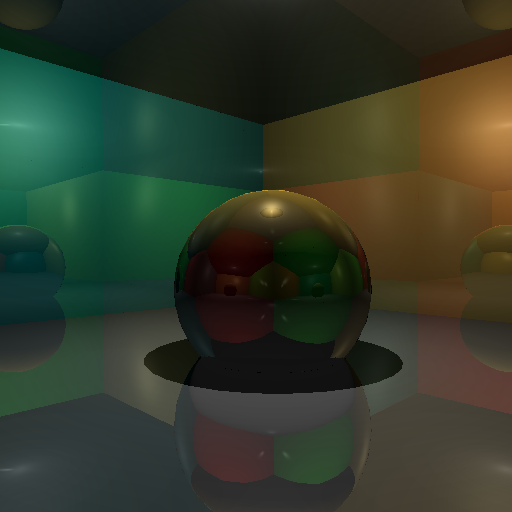
\includegraphics[width=4.0cm]{Images/Cornell_Preview}
        \captionof{figure}{\textsc{Cornell}}
    \end{minipage}
    \begin{minipage}{0.725\linewidth}
        \centering
        \fontencoding{T1}
        \fontseries{m}
        \fontshape{sc}
        \fontsize{8}{10}
        \selectfont
        \begin{tabular}[h]{l|rrrr}
            \multicolumn{1}{c|}{\textsc{Office}} & \textsc{Level 4} & \textsc{Level 3} & \textsc{Level 2} & \textsc{Level 1}\\
            \hline
            \emph{RAH Algorithm} & & \\
            \hline
            \quad \# Sh Intersections   & 3168		& 50688		& 760128	& 7732000	\\
            \quad \# Sh Misses          & 0		    & 3180		& 276878	& 6808346	\\
            \quad \# Sh Hits            & 3168		& 47508		& 483250	& 923654	\\
            & & \\
            \quad \# Re Intersections   & 6336		& 101376	& 1622016	& 23053680	\\
            \quad \# Re Misses          & 0	        & 0	        & 181161	& 20614507	\\
            \quad \# Re Hits            & 6336		& 101376	& 1440855	& 2439173	\\
            \hline
            \emph{Our Algorithm} & & \\
            \hline
            \quad \# Sh Intersections   & 3168	    & 50688		& 498352	& 2577680	\\
            \quad \# Sh Misses          & 0		    & 19541		& 337247	& 1856187	\\
            \quad \# Sh Hits            & 3168		& 31147	    & 161105	& 721493	\\
            & & \\
            \quad \# Re Intersections   & 6336		& 101376	& 1620432	& 11466336	\\
            \quad \# Re Misses          & 0		    & 99	    & 903786	& 9374256	\\
            \quad \# Re Hits            & 6336		& 101277	& 716646	& 2092080	\\            
        \end{tabular}
        \label{table:cornell-d16-n4-results}
        \captionof{table}{\textsc{Cornell} Division 16 Depth 4 Test Results.}
    \end{minipage}
\end{figure}

\subsubsection{Sponza}

% Sponza Discussion

Comparing our algorithm with the RAH algorithm we can see that our algorithm computes 35,86\% less intersections than RAH on this scene. 97,62\% less than a brute force approach (see Table~\ref{table:sponza-d16-n4-results} and Table~\ref{table:results-d16-n4}).

% Sponza Table and Figure

\begin{figure}[!htb]
    \begin{minipage}{0.25\linewidth}
        \centering
        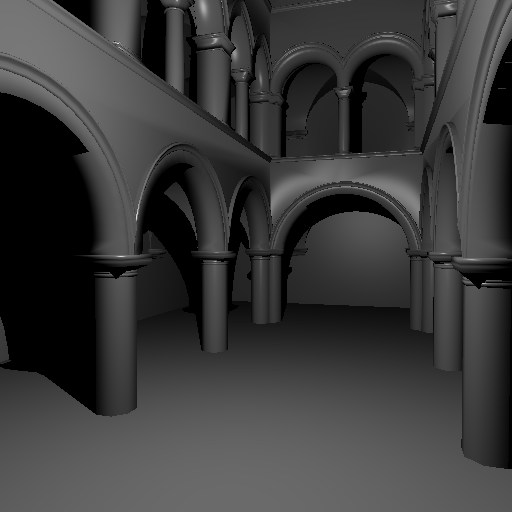
\includegraphics[width=4.0cm]{Images/Sponza_Preview}
        \captionof{figure}{\textsc{Sponza}}
    \end{minipage}
    \begin{minipage}{0.725\linewidth}
        \centering
        \fontencoding{T1}
        \fontseries{m}
        \fontshape{sc}
        \fontsize{8}{10}
        \selectfont
        \begin{tabular}[h]{l|rrrr}
            \multicolumn{1}{c|}{\textsc{Office}} & \textsc{Level 4} & \textsc{Level 3} & \textsc{Level 2} & \textsc{Level 1}\\
            \hline
            \emph{RAH Algorithm} & & \\
            \hline
            \quad \# Sh Intersections   & 265800	& 4252800	& 66981600	& 554494192	\\
            \quad \# Sh Misses          & 0		    & 66450		& 32325713	& 544455870	\\
            \quad \# Sh Hits            & 265800	& 4186350	& 34655887	& 10038322	\\
            & & \\
            \hline
            \emph{Our Algorithm} & & \\
            \hline
            \quad \# Sh Intersections   & 265800	& 4252800	& 29037376	& 102667568	\\
            \quad \# Sh Misses          & 0	        & 2437964   & 22620653	& 97483134	\\
            \quad \# Sh Hits            & 265800	& 1814836	& 6416723	& 5184434	\\
        \end{tabular}
        \label{table:sponza-d16-n4-results}
        \captionof{table}{\textsc{Sponza} Division 16 Depth 4 Test Results.}
    \end{minipage}
\end{figure}

\subsection{Hierarchy Traversal Discussion - Subdivision 16 Depth 4}

% Comparison Table

\begin{table}[!htb]
    \begin{center}
    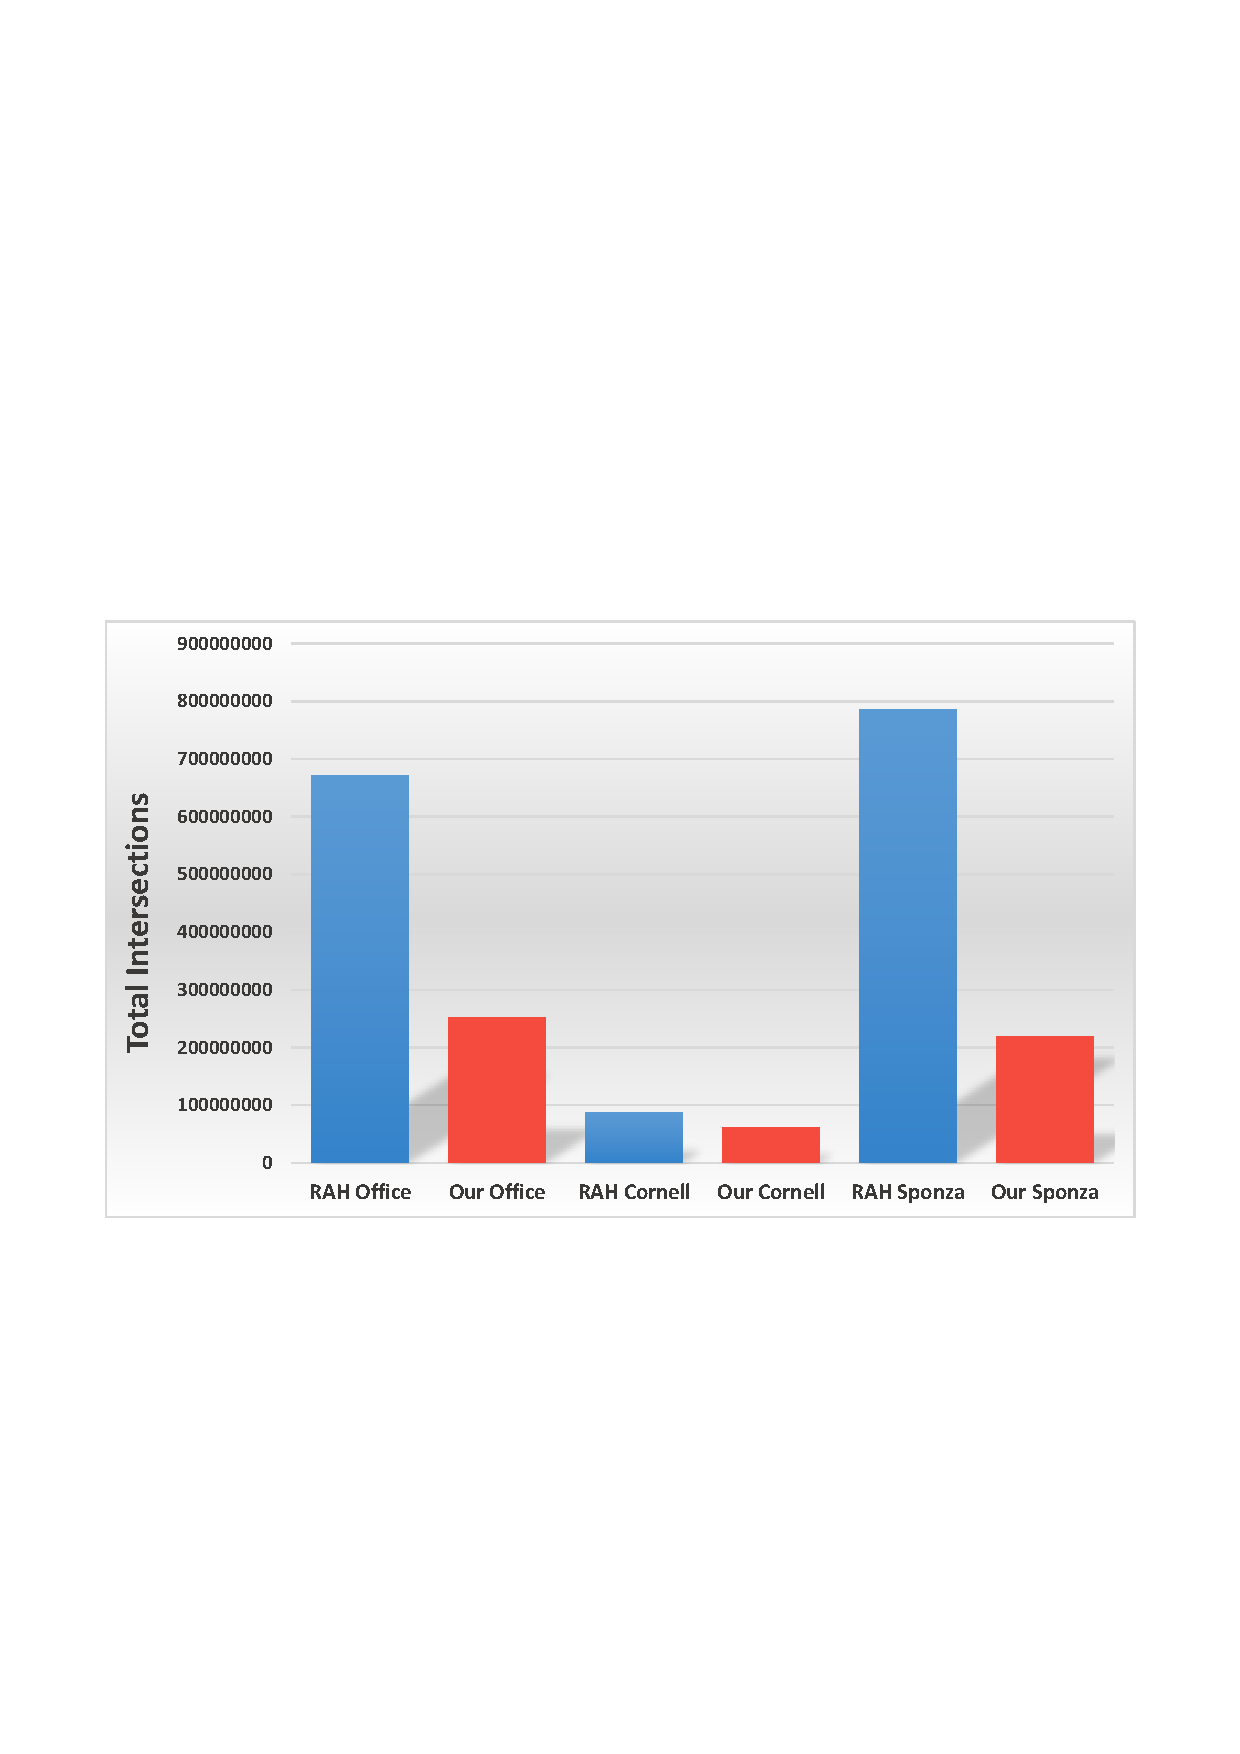
\includegraphics[width=0.85\textwidth]{Images/Chart_N16_D4}
    \vskip 2em
    \fontencoding{T1}
    \fontseries{m}
    \fontshape{sc}
    \fontsize{8}{10}
    \selectfont
    \begin{tabular}{l|rrrrrr}
    & \multicolumn{2}{c}{\textsc{Office}} & \multicolumn{2}{c}{\textsc{Cornell}} & \multicolumn{2}{c}{\textsc{Sponza}} \\
    \textsc{Algorithm} & \textsc{Total \# isect} & \textsc{Relative \%} & \textsc{Total \# isect} & \textsc{Relative \%} & \textsc{Total \# isect} & \textsc{Relative \%} \\
        \hline
        \emph{Brute Force}     & 9133132168         & 100\%           & 606911976         & 100\%           & 17058578850         & 100\% \\
        \emph{RAH Algorithm}   & 671594400			& 7.35\%          & 87134624		  & 14.36\%         & 786607544		      & 4.61\% \\
        \emph{Our Algorithm}   & \textbf{252175344} & \textbf{2.76\%} & \textbf{61341536} & \textbf{10.11\%} & \textbf{219174488} & \textbf{1.28\%} \\
    \end{tabular}
    \end{center}
    \caption{\label{table:results-d16-n4}
    \small\textsc{Office} (251546 shadow rays), \textsc{Cornell} (242015 shadow \& 524288 reflection rays), \textsc{Sponza} (256713 shadow rays) rendering performance  using node subdivision 16 and hierarchy depth 4.}
\end{table}

\begin{figure}[!htb]
    \begin{center}
    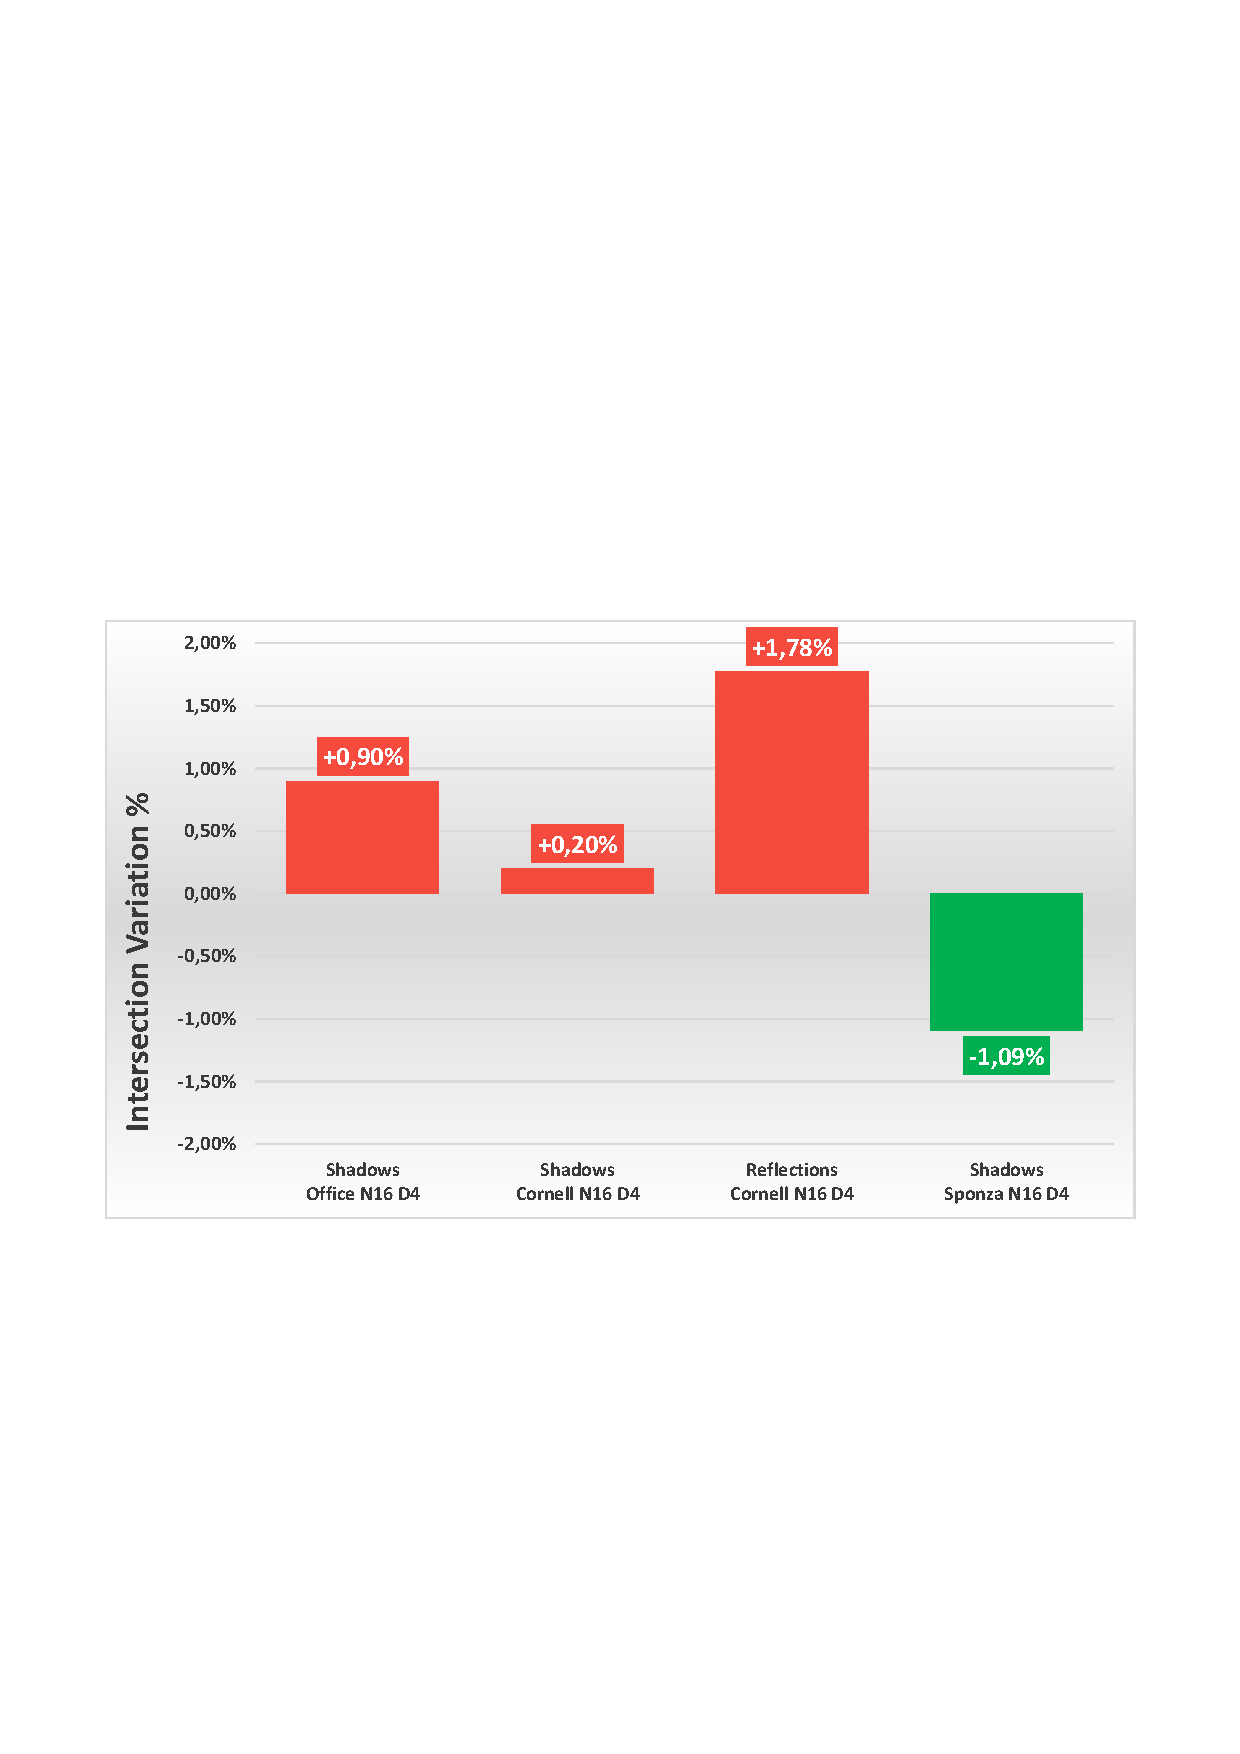
\includegraphics[width=0.70\textwidth]{Images/Chart_Comparison_N8_D2_N16_D4}
    \label{fig:comparison-results-d8-n2-d16-n4}
    \caption{Configuration Comparison between Node Subdivision 8 with Hierarchy Depth 2 and Node Subdivision 16 with Hierarchy Depth 4.}
    \end{center}
\end{figure}

For this set of tests we used a node subdivision of 16 and a hierarchy depth of 3. This means that every node in the upper levels of the hierarchy consists of 16 nodes in the level directly below. We compared this configuration with the baseline configuration of node subdivision of 8 and hierarchy depth of 2.

\subsubsection{Office}

For the final configuration the Office scene calculated less intersections the RAH algorithm (see Table~\ref{table:office-d16-n4-results}). We compute 62.45\% less intersections than RAH on this scene and 97,24\% less than a brute force approach. There is yet another increase of 0.70\% when compared to the baseline (from 1.86\% to 2.75\%) (see Figure~\ref{fig:comparison-results-d8-n2-d16-n3}). 

\subsubsection{Cornell}

For the final test for the Cornell scene we compute 29,60\% less intersections overall (shadow and reflection rays combined) than the RAH algorithm and 89,89\% less than the brute force approach (see Table~\ref{table:cornell-d16-n4-results}). When we compare these results with the baseline configuration we get an increase of 0.13\%, from 7.45\% to 7.66\% for shadow rays and from 9.46\% to 11.25\% for reflection rays (see Figure~\ref{fig:comparison-results-d8-n2-d16-n4}).

\subsubsection{Sponza}

For the final test using the Sponza scene we computed 72,14\% less intersection tests than RAH and 98,68\% than the brute force approach (see Table~\ref{table:sponza-d16-n4-results}). The number of intersection tests was reduced once again, going from the baseline 2.38\% to 1.28\% (see Figure~\ref{fig:comparison-results-d8-n2-d16-n4}). We increased the depth from the previous configuration but we got a small increase in the intersection tests. This indicates that the previous configuration is the break point after which increasing the depth stops yielding benefits for this scene.

%%%%%%%%%%%%%%%%%%%%%%%%%%%%%%%%%%%%%%%%%%%%%%%%%%%%%%%%%%%%%%%%%%%%%%%%%%%%%%%%%%%%%%%%%%%%%%%%%%%%%%%%%%%%%%%%%%%%%%%%%%%%%%%%%%

\subsection{Rendering Time Results}

For this set of tests we used a node subdivision of 8 and a hierarchy depth of 2. This means that every node in the upper levels of the hierarchy consists of 16 nodes in the level directly below. The tests were run over the course of 58 frames and the results for each phase are the average of these 58 frames. 

\subsubsection{Office}

\begin{figure}[!htb]
    \begin{minipage}{0.25\linewidth}
        \centering
        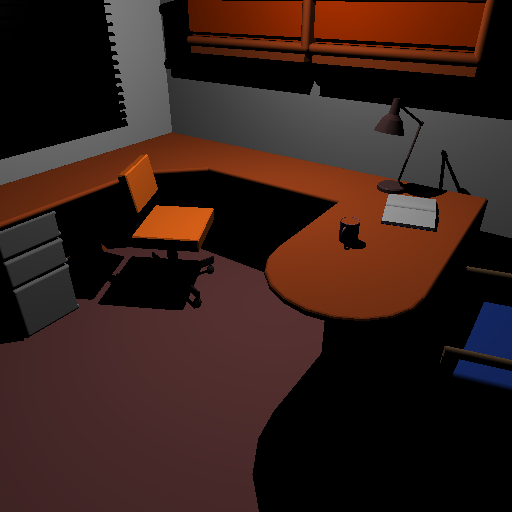
\includegraphics[width=4.0cm]{Images/Office_Preview}
        \captionof{figure}{\textsc{Office}}
    \end{minipage}
    \begin{minipage}{0.725\linewidth}
        \centering
        \fontencoding{T1}
        \fontseries{m}
        \fontshape{sc}
        \fontsize{8}{10}
        \selectfont
        \begin{tabular}[h]{l|rrrr}
            \multicolumn{1}{c|}{\textsc{Office}} & \textsc{Total Time (ms)} & \textsc{Relative Time (\%)}\\
            \hline
            \emph{RAH Algorithm (618 ms per Frame)} & & \\
            \hline
            \quad \# Ray Creation               & 40,240	& 0,11\%	\\
            \quad \# Ray Compression            & 0,000     & 0,00\%	\\
            \quad \# Ray Sorting                & 0,000	    & 0,00\%    \\
            \quad \# Ray Decompression          & 0,000	    & 0,00\%    \\
            \quad \# Hierarchy Creation         & 122,165	& 0,34\%    \\
            \quad \# Hierarchy Traversal        & 30394,169	& 84,77\%   \\
            \quad \# Final Intersection Tests   & 4428,185	& 12,35\%	\\
            & & \\
            \hline
            \emph{Our Algorithm (316 ms per Frame)} & & \\
            \hline
            \quad \# Ray Creation               & 40,433	& 0,22\%	\\
            \quad \# Ray Compression            & 16,651    & 0,09\%	\\
            \quad \# Ray Sorting                & 11,822	& 0,06\%    \\
            \quad \# Ray Decompression          & 99,721	& 0,54\%    \\
            \quad \# Hierarchy Creation         & 130,626	& 0,71\%    \\
            \quad \# Hierarchy Traversal        & 13918,797	& 75,76\%   \\
            \quad \# Final Intersection Tests   & 3355,308	& 18,26\%	\\
        \end{tabular}
        \label{table:office-time-results}
        \captionof{table}{\textsc{Office} Rendering Time Results.}
    \end{minipage}
\end{figure}

For this scene we can see that the major time consuming steps are in fact the hierarchy traversal and the final intersection tests. The biggest difference between our algorithm and the RAH algorithm resides in the time spent traversing the hierarchy. While our algorithm only needs 13918 milliseconds, the RAH algorithm requires 30394 milliseconds, which is about 215\% more. This increased time traversing the hierarchy amounts to about 100\% more time to render each frame (see Table~\ref{table:office-time-results}).

\vfill

\pagebreak

\subsubsection{Cornell}

\begin{figure}[!htb]
    \begin{minipage}{0.25\linewidth}
        \centering
        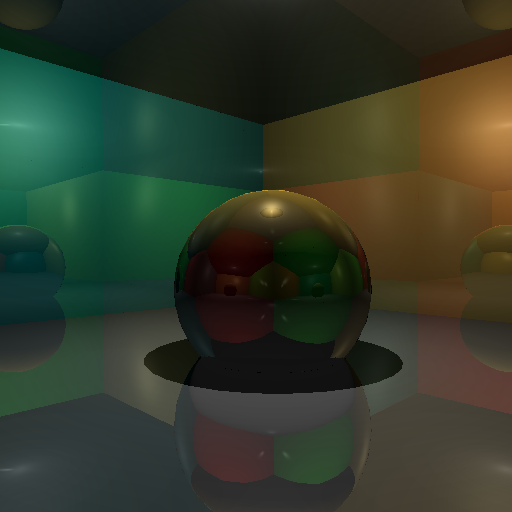
\includegraphics[width=4.0cm]{Images/Cornell_Preview}
        \captionof{figure}{\textsc{Cornell}}
    \end{minipage}
    \begin{minipage}{0.725\linewidth}
        \centering
        \fontencoding{T1}
        \fontseries{m}
        \fontshape{sc}
        \fontsize{8}{10}
        \selectfont
        \begin{tabular}[h]{l|rrrr}
            \multicolumn{1}{c|}{\textsc{Cornell}} & \textsc{Total Time (ms)} & \textsc{Relative Time (\%)}\\
            \hline
            \emph{RAH Algorithm (93 ms per Frame)} & & \\
            \hline
            \quad \# Ray Creation               & 125,731	& 2,16\%	\\
            \quad \# Ray Compression            & 0,000     & 0,00\%	\\
            \quad \# Ray Sorting                & 0,000	    & 0,00\%    \\
            \quad \# Ray Decompression          & 0,000	    & 0,00\%    \\
            \quad \# Hierarchy Creation         & 366,984	& 6,29\%    \\
            \quad \# Hierarchy Traversal        & 2717,309	& 46,59\%   \\
            \quad \# Final Intersection Tests   & 2208,936	& 37,88\%	\\
            & & \\
            \hline
            \emph{Our Algorithm (100 ms per Frame)} & & \\
            \hline
            \quad \# Ray Creation               & 128,134	& 2,38\%	\\
            \quad \# Ray Compression            & 53,916    & 1,00\%	\\
            \quad \# Ray Sorting                & 50,970    & 0,95\%    \\
            \quad \# Ray Decompression          & 251,946   & 4,68\%    \\
            \quad \# Hierarchy Creation         & 407,090   & 7,57\%    \\
            \quad \# Hierarchy Traversal        & 1776,750  & 33,03\%   \\
            \quad \# Final Intersection Tests   & 2175,057  & 40,43\%	\\
        \end{tabular}
        \label{table:cornell-time-results}
        \captionof{table}{\textsc{Cornell} Rendering Time Results.}
    \end{minipage}
\end{figure}

Much like Office, the Cornell scene takes most of its rendering time traversing the hierarchy and calculating the final intersection tests. However due to the lower geometric complexity of the scene the absolute values aren't as high. The traversal takes 2717 milliseconds for the RAH algorithm and 1700 for our algorithm, which is a significant reduction (see Table~\ref{table:cornell-time-results}).

\vfill

\pagebreak

\subsubsection{Sponza}

\begin{figure}[!htb]
    \begin{minipage}{0.25\linewidth}
        \centering
        \includegraphics[width=4.0cm]{Images/Sponza_Preview}
        \captionof{figure}{\textsc{Sponza}}
    \end{minipage}
    \begin{minipage}{0.725\linewidth}
        \centering
        \fontencoding{T1}
        \fontseries{m}
        \fontshape{sc}
        \fontsize{8}{10}
        \selectfont
        \begin{tabular}[h]{l|rrrr}
            \multicolumn{1}{c|}{\textsc{Sponza}} & \textsc{Total Time (ms)} & \textsc{Relative Time (\%)}\\
            \hline
            \emph{RAH Algorithm} & & \\
            \hline
            \quad \# Ray Creation               & 41,215	& 0,07\%	\\
            \quad \# Ray Compression            & 0,000     & 0,00\%	\\
            \quad \# Ray Sorting                & 0,000	    & 0,00\%    \\
            \quad \# Ray Decompression          & 0,000	    & 0,00\%    \\
            \quad \# Hierarchy Creation         & 126,499	& 0,23\%    \\
            \quad \# Hierarchy Traversal        & 49537,627	& 89,25\%   \\
            \quad \# Final Intersection Tests   & 4995,089	& 9,00\%	\\
            & & \\
            \hline
            \emph{Our Algorithm} & & \\
            \hline
            \quad \# Ray Creation               & 41,500	& 0,08\%	\\
            \quad \# Ray Compression            & 17,151    & 0,03\%	\\
            \quad \# Ray Sorting                & 12,696	& 0,02\%    \\
            \quad \# Ray Decompression          & 98,617	& 0,19\%    \\
            \quad \# Hierarchy Creation         & 137,835	& 0,26\%    \\
            \quad \# Hierarchy Traversal        & 46867,912	& 89,65\%   \\
            \quad \# Final Intersection Tests   & 4367,193	& 8,35\%	\\
        \end{tabular}
        \label{table:sponza-time-results}
        \captionof{table}{\textsc{Sponza} Rendering Time Results.}
    \end{minipage}
\end{figure}

Finally for the Sponza scene we still see a similar relative time being spent in the traversal of the hierarchy as in the previous scenes. Even though the Sponza scene isn't subdivided into separate object meshes, we still manage to outperform RAH while traversing the hierarchy (see Table~\ref{table:sponza-time-results}). 

\vfill

\pagebreak

%%%%%%%%%%%%%%%%%%%%%%%%%%%%%%%%%%%%%%%%%%%%%%%%%%%%%%%%%%%%%%%%%%%%%%%%%%%%%%%%%%%%%%%%%%%%%%%%%%%%%%%%%%%%%%%%%%%%%%%%%%%%%%%%%%

\subsection{Test Results Global Discussion}

\subsubsection{Configuration Tests}

For the Office scene the configuration tests indicated that the optimal configuration is in fact the baseline configuration used, using node subdivision of 8 and hierarchy depth of 2. However this is reliant on the hashing function used, which means that if a better hashing function is used the optimal configuration may be different. 

\medskip

For the Cornell scene there was always an increase for every configuration when compared with the baseline configuration. However this increase was more significant for the reflection rays. This is due to the fact that reflection rays are much less coherent than shadow rays, which leads to bigger nodes when combining such rays. Much like the shadow rays however using better hashing functions can mitigate this effect.

\medskip

Finally for the Sponza scene we noticed a reverse trend compared to the remaining scenes. This is due to the fact that the scene itself isn't subdivided into several objects, making the use of bounding spheres useless. As such, only the higher levels of the hierarchy were culling the number of potential intersection tests, which means that as we increased the hierarchy's depth this mitigation effect would be increased until we reached a certain break point, like it was noted before. Since this scene is an outlier however it is safe to assume if it was subdivided into several objects, much like the Office scene, the optimal configuration would be the baseline configuration used for the tests.

\subsubsection{Rendering Time Tests}

Regarding the rendering time tests, it is notable that even though we managed to significantly reduce the total number of intersection tests the hierarchy traversal still takes up most of the rendering time. This leads us to believe that if we can optimize the traversal step, either by culling more intersection tests at the early stages or by making the implementation more efficient we can get a significant reduction in the time necessary for the two final phases of our algorithm. % file "Thesis_Evaluation.tex"
\cleardoublepage

%%%%%%%%%%%%%%%%%%%%%%%%%%%%%%%%%%%%%%%%%%%%%%%%%%%%%%%%%%%%%%%%%%%%%%%%
%                                                                      %
%     File: Thesis_Conclusions.tex                                     %
%     Tex Master: Thesis.tex                                           %
%                                                                      %
%     Author: Andre C. Marta                                           %
%     Last modified :  2 Jul 2015                                      %
%                                                                      %
%%%%%%%%%%%%%%%%%%%%%%%%%%%%%%%%%%%%%%%%%%%%%%%%%%%%%%%%%%%%%%%%%%%%%%%%

\chapter{Conclusions}
\label{chapter:conclusions}

Insert your chapter material here...


% ----------------------------------------------------------------------
\section{Achievements}
\label{section:achievements}

The major achievements of the present work...


% ----------------------------------------------------------------------
\section{Future Work}
\label{section:future}

A few ideas for future work...

 % file "Thesis_Conclusions.tex"
\cleardoublepage

% ----------------------------------------------------------------------
%  Bibliography
% ----------------------------------------------------------------------

% Add entry in the table of contents as chapter
\phantomsection
\addcontentsline{toc}{chapter}{\bibname}

\bibliographystyle{abbrvunsrtnat}

% External bibliography database file in the BibTeX format
\bibliography{Thesis_Bibliography} % file "Thesis_Bibliography.bib"

\cleardoublepage

% ----------------------------------------------------------------------
%  Appendix (optional)
%
%  CAUTION: 1) the main document (up to the conclusions) shall not exceed 80 pages
%           2) the document shall not exceed a total of 100 pages (per IST regulations)
% ----------------------------------------------------------------------
\appendix

% add page number prefix according to apendix chapter (optional)
%\renewcommand{\thepage}{\thechapter.\arabic{page}}

% re-set arabic numbering (A.1,A.2,...) (optional, use only if chapter prefix is added)
%\setcounter{page}{1}

%%%%%%%%%%%%%%%%%%%%%%%%%%%%%%%%%%%%%%%%%%%%%%%%%%%%%%%%%%%%%%%%%%%%%%%%
%                                                                      %
%     File: Thesis_Appendix.tex                                      %
%     Tex Master: Thesis.tex                                           %
%                                                                      %
%     Author: Andre C. Marta                                           %
%     Last modified :  2 Jul 2015                                      %
%                                                                      %
%%%%%%%%%%%%%%%%%%%%%%%%%%%%%%%%%%%%%%%%%%%%%%%%%%%%%%%%%%%%%%%%%%%%%%%%

\chapter{Rendered Images}
\label{chapter:rendered-images}

\begin{center}
    \includegraphics[scale=0.75]{Images/Office_Preview}  \\
    \textsc{Office} \\
    \vskip 1em

    \includegraphics[scale=0.75]{Images/Cornell_Preview} \\
    \textsc{Cornell} \\
    \vskip 1em

    \includegraphics[scale=0.75]{Images/Sponza_Preview}  \\
    \textsc{Sponza} \\
    \vskip 1em
\end{center}
 % file "Thesis_Appendix.tex"
\cleardoublepage

% re-set arabic numbering (B.1,B.2,...) (optional, use only if chapter prefix is added)
%\setcounter{page}{1}

%%%%%%%%%%%%%%%%%%%%%%%%%%%%%%%%%%%%%%%%%%%%%%%%%%%%%%%%%%%%%%%%%%%%%%%%%
%                                                                      %
%     File: Thesis_Appendix_B.tex                                      %
%     Tex Master: Thesis.tex                                           %
%                                                                      %
%     Author: Andre C. Marta                                           %
%     Last modified :  2 Jul 2015                                      %
%                                                                      %
%%%%%%%%%%%%%%%%%%%%%%%%%%%%%%%%%%%%%%%%%%%%%%%%%%%%%%%%%%%%%%%%%%%%%%%%

\chapter{Technical Datasheets}
\label{chapter:appendixDatasheets}

It is possible to add PDF files to the document, such as technical sheets of some equipment used in the work.

% ----------------------------------------------------------------------
\section{Some Datasheet}
\label{section:datasheet}

% See more options to include PDF files in
% http://mirror.unl.edu/ctan/macros/latex/contrib/pdfpages/pdfpages.pdf
\includepdf[pages={1-2},nup=1x2,landscape=true]{Figures/SolarCell_Sunpower_C60.pdf}

 % file "Thesis_Appendix_B.tex"
%\cleardoublepage

% ----------------------------------------------------------------------
\end{document}
% ----------------------------------------------------------------------

